\documentclass[12pt]{report}
\usepackage{report}
%%%%%%%%%%% langage
\usepackage[french]{babel}

%%%%%%%%%%%%ù autres packages
\usepackage[acronym]{glossaries}
\usepackage{rotating}
\usepackage{float}
\usepackage{siunitx}
\usepackage{array}
\usepackage[justification=centering]{caption}
\captionsetup[figure]{font=small}
\usepackage{booktabs}
\usepackage[table,xcdraw]{xcolor}
\usepackage{chngcntr}
\usepackage[utf8]{inputenc}
\usepackage{listings}
\usepackage{subcaption}
\usepackage{indentfirst}
\usepackage{enumitem}
\usepackage{booktabs}
\usepackage{multirow}
\usepackage{flafter}
\usepackage{hyperref}
\usepackage[outputdir=../]{minted}
\usepackage{lipsum}

%%% Times New Roman font
\usepackage{newtxtext}
\usepackage{newtxmath}

%%%%%%%%%%%%%% alphabet 
\usepackage{lettrine}
\usepackage{xcolor}

%%%%%%%%%%
\usepackage{titling}
\usepackage{mdframed}
\usepackage{xcolor}

%%%%%%%%%%%%%%%%%%%%% MULTI COL 
\usepackage{multicol}
%%%%%%%%%%%%%%%% org
\usepackage{tikz}
\usetikzlibrary{calc}

\usepackage{enumitem}
\usepackage{array}
\usepackage{geometry}
\usepackage{graphicx}
\setstretch{1.5}






\hypersetup{
    colorlinks=true,
    linkcolor=blue,
    filecolor=magenta,      
    urlcolor=blue,
    citecolor=blue,
    pdfpagemode=FullScreen,
}
\usepackage{lettrine}


\setlength{\parindent}{0.6cm}

\setcounter{secnumdepth}{3} % subheadings
\setlength{\cfttabindent}{0pt} % tableaux
\setlength{\cftfigindent}{0pt} % figures

% Set this up
\title{SA}
\author{am.elmah}

\date{\today}
\counterwithout{figure}{section}
\counterwithin{figure}{chapter}
\counterwithout{table}{section}
\counterwithin{table}{chapter}




\begin{document}

\addtocontents{toc}{\protect  \hfill \par \bigskip}

%\input{sec/titlepage}
% Numérotation
\pagenumbering{roman} % roman 
% DEDICACE
\newpage

\chapter*{DEDICACE}

Je dédie ce travail à ma mère, celle qui éclaire mon chemin dans les moments sombres, à mon père, mon ancre dans les tempêtes de la vie, à mes sœurs Imane et Oumaima, ainsi qu'à mon frère Zakariaa, les piliers solides sur lesquels je m'appuie. Je souhaite également dédier ce travail à Salima, mon amie sur qui je peux toujours compter, quelles que soient les circonstances.

\rightline{— \textbf{ BOUKOULLA Ouissal}} 

\vspace{4cm}
Je dédie ce travail à mes chers parents. C'est grâce à vous, et pour vous, que je suis là aujourd'hui. \\
\rightline{— \textbf{ EL MAHRAOUI Amal}} 


%\textbf{Date}
%\hfill
%\textbf{ Candidate}



% REMERCIEMENT
\newpage
\chapter*{REMERCIEMENT}
\addcontentsline{toc}{section}{REMERCIEMENT}

\normalsize
Je remercie Dieu tout-Puissant de m'avoir donné la santé et le bien être. \\
Je tiens à exprimer ma profonde gratitude à Monsieur  \textbf{ZANNOU Abderrahim}, notre encadrant,  pour son suivi attentif. Sans ses conseils et ses efforts, nous n'aurions pas pu mener à bien ce projet.\\ 
Je souhaite également remercier notre co-encadrante, \textbf{Mme. BOUAROUROU Soukaina}, pour sa précieuse contribution. Sa touche unique a enrichi notre travail. Merci pour tous vos efforts et votre engagement.\\
Un merci tout particulier aux membres du jury Monsieur \textbf{SOUFI Adil} et \textbf{SRAI Aziz} pour avoir bien voulu examiner et évaluer ce modeste travail.\\
Je remercie infiniment Monsieur \textbf{FAHIM Mohamed} pour ses compétences et ses précieux conseils. Merci pour l'impact que vous avez eu sur mon parcours académique, ainsi que pour votre motivation et votre soutien constant.\\
Mes remerciements les plus chaleureux vont à mes \textbf{chers parents}, pour leur aide précieuse, leur soutien moral et leurs nombreux encouragements,  ainsi qu'à ma très belle sœur \textbf{Hanan}, qui a été mon pilier, me soutenant et m'encourageant à chaque étape de mon parcours. Merci pour tout ce que vous avez fait pour moi et merci d'être toujours de mes cotés.  \\ 
Un sincère merci à ma collègue \textbf{BOUKOULLA Ouissal} pour ses efforts et sa collaboration précieuse dans ce projet.\\
Je remercie également mes collègues, mes professeurs de la formation et tous ceux qui ont marqué mon parcours, que ce soit par un conseil, une motivation ou un mot aimable.  \\
Merci à vous tous pour cette expérience inoubliable.

\rightline{— \textbf{ EL MAHRAOUI Amal}}


% Acknowledgments

\newpage
\chapter*{REMERCIEMENT}
\addcontentsline{toc}{section}{REMERCIEMENT}

\normalsize
Je remercie avant tout \textbf{Dieu}, pour m'avoir accordé la force, la patience et la sagesse nécessaires pour mener à bien ce projet. Sans Sa bénédiction et Sa guidance, rien de tout cela n'aurait été possible \\
Avant tout, je remercie chaleureusement Monsieur \textbf{Abderrahim ZANNOU}, notre encadrant, dont les conseils judicieux, le soutien indéfectible et les encouragements constants ont illuminé chaque étape de ce projet. Sa rigueur scientifique exemplaire et son expertise ont été indispensables à la réussite de ce travail.\\
J’adresse également mes remerciements à Madame \textbf{Soukaina BOUAROUROU}, en tant que co-encadrante. Son guide, son support et ses conseils ont été essentiels pour que ce travail puisse voir le jour.\\
Un immense merci à Monsieur \textbf{Adil SOUFI} pour sa vision et son dévouement dans la création et l’évolution de cette filière, qui ont profondément changé le cours de ma vie et m’ont ouvert les portes d’un domaine aussi passionnant.\\
Mes sincères remerciements vont à mes professeurs de la formation, un par un, pour leur engagement et leur soutien tout au long de mon parcours. Leur expertise et leur dévouement ont été des sources d’inspiration qui ont enrichi mon expérience et m’ont permis de progresser tant sur le plan académique que personnel.\\
Je souhaite également exprimer ma profonde gratitude aux membres du jury pour leur temps précieux et leur expertise. Leurs analyses éclairées, leurs questions pertinentes et leurs remarques constructives ont considérablement enrichi ce travail et m'ont permis d'explorer de nouvelles perspectives. Leur engagement et effort à l'évaluation de ce projet sont vivement appréciés.\\
Je suis profondément reconnaissante d’avoir ma famille à mes côtés : mes \textbf{chers parents}, \textbf{mes sœurs}, et \textbf{mon frère}. Leur amour inconditionnel et leur présence bienveillante ont été ma source d’inspiration. Je suis honorée de pouvoir partager mes réalisations avec vous. Merci pour tout ce que vous avez fait pour moi.\\
Enfin, je ne saurais terminer sans remercier mes amis et mes collègues. Leurs présences, leurs échanges enrichissants et les moments de complicité partagés ont été autant de rayons de soleil dans mon parcours. Un remerciement particulier à ma collègue dans ce travail, Mlle \textbf{Amal EL MAHRAOUI}. Ses idées novatrices et son travail acharné ont été une source d’inspiration constante. Merci pour cette expérience enrichissante et pour avoir partagé ce parcours avec moi.\\
Je suis reconnaissante à tous ceux qui m'ont soutenu, même par un mot aimable. \\

\rightline{— \textbf{ BOUKOULLA Ouissal}} 



% RESUME
\input{sec/resumé}
% ABSTRACT
\newpage
\chapter*{ABSTRACT}
\addcontentsline{toc}{section}{ABSTRACT}
Understanding the opinions or views of others on products or services and grasping their emotions and attitudes towards a social event has been an essential informational aspect, especially during the decision-making process.  People are highly interested in others' opinions across various domains; they seek out reviews before making a purchase or utilizing a service. \\
This report focuses on analyzing the performance of various machine learning models for sentiment classification of Twitter messages (tweets) and the natural language processing (NLP) methods employed. A comparative study of multiple machine learning algorithms is conducted, leveraging different preprocessing techniques, including lemmatization and stemming, as well as various text representation techniques applied to two datasets: one concerning sentiments (positive and negative) and the other emotions (joy, sadness, fear, etc.). This study reveals that the models' performance depends on numerous factors such as preprocessing techniques, text representation methods, the nature of datasets, and the algorithms employed. Additionally, a web application has been developed using Django to provide an intuitive user interface, demonstrating the practical utility of this approach.\\
\emph{{\textbf{Keywords:}} NLP, Sentiment Analysis, Machine Learning, Emotions, Django.}

{

% coleur
\hypersetup{linkcolor=black}

\begin{center}
  
  \setlength{\parskip}{0em}
  \renewcommand\contentsname{TABLE DES MATIÈRES} % Change le texte du titre de la table des matières
  \tableofcontents
\end{center}

% List des figures 

\newpage
\listoffigures 
\addcontentsline{toc}{section}{LISTE DES FIGURES}
% List des tableaux

\newpage
\listoftables 
\addcontentsline{toc}{section}{LISTE DES TABLEAUX}
}
% List des abbreviations
\clearpage

\chapter*{GLOSSAIRE}
\begin{description}[style=multiline, leftmargin=2cm, labelindent=1cm]
    \item[IA] \hfill \\
    \textbf{Intelligence Artificielle} \hfill \\
    (Artificial Intelligence)
    \item[ML] \hfill \\
    \textbf{Apprentissage Automatique} \hfill \\
    (Machine Learning)
    \item[DL] \hfill \\
    \textbf{Apprentissage Profond} \hfill \\
    (Deep Learning)
    \item[SA] \hfill \\
    \textbf{Analyse des Sentiments} \hfill \\
    (Sentiment Analysis)
    \item[NLP] \hfill \\
    \textbf{Traitement du Langage Naturel} \hfill \\
    (Natural Language Processing)
    \item[RNN] \hfill \\
    \textbf{Réseau de Neurones Récurent} \hfill \\
    (Recurrent Neural Network)
    \item[CNN] \hfill \\
    \textbf{Réseau de Neurones Convolutif} \hfill \\
    (Convolutional Neural Network)
    \item[BoW] \hfill \\
    \textbf{Sac de Mots} \hfill \\
    (Bag of Words)
    
    \item[TF-IDF] \hfill \\
    \textbf{Terme Fréquence-Inverse de Document} \hfill \\
    (Term Frequency-Inverse Document Frequency)
    
    \item[LSTM] \hfill \\
    \textbf{Mémoire à Long et Court Terme} \hfill \\
    (Long-Short Term Memory)
    
    \item[SVM] \hfill \\
    \textbf{Machine à Vecteurs de Support} \hfill \\
    (Support Vector Machine)
    
    \item[nu-SVC] \hfill \\
    \textbf{Classification par Vecteurs de Support avec Nu} \hfill \\
    (Nu-Support Vector Classification)
    
    \item[RL] \hfill \\
    \textbf{Régression Logistique} \hfill \\
    (Logistic Regression)
    
    \item[CNB] \hfill \\
    \textbf{Bayésien Naïf Complémentaire} \hfill \\
    (Complementary Naive Bayes)
    
    \item[MNB] \hfill \\
    \textbf{Bayésien Naïf Multinomial} \hfill \\
    (Multinomial Naive Bayes)
\end{description}



% Intro 
\clearpage
\phantomsection
\addcontentsline{toc}{chapter}{INTRODUCTION GÉNÉRALE}
\chapter*{INTRODUCTION GÉNÉRALE}

\lettrine[lines=3,lraise=0.1,findent=0.6em]{L'}{analyse} des sentiments, également connue sous le nom de mining d’opinions, est le processus qui consiste à extraire des informations subjectives, à partir des textes, généralement des opinions, des émotions, ou des attitudes exprimées, par des individus à l’égard d’un sujet particulier. Avec la prolifération des réseaux sociaux, cette discipline est devenue essentielle pour comprendre les tendances et les opinions qui circulent en ligne. Aujourd’hui chaque page web dispose d’une section permettant aux utilisateurs de laisser leurs commentaires, ce qui n’était pas possible avant quelques années. Un exemple notable de ces pages web, Twitter ou bien X qu’est à l’origine une plateforme micro-blogging très populaire, Elle a connu une croissance régulière ces dernières années, est devenue un point de rencontre d’une gamme diversifiée des personnes (politiciens, professionnels, célébrités, étudiants, …), cette popularité se traduit par une énorme quantité d’informations couvrant une large gamme de sujets allant de bien-être vers les marques, la politique, les événements sociaux, ce qui rend Twitter un outil puissant pour extraire des tweets afin de faire des prédictions sur sentiments et les opinions des utilisateurs, ces applications présentent un intérêt commercial au entreprises et aux chercheurs pour prendre des décisions opérationnelle.


De nombreux modèles et services différents pour effectuer l'analyse des sentiments sont disponibles. Il est souvent difficile de choisir le bon pour le cas d'utilisation qui nous intéresse. Cette thèse analyse les techniques pertinentes qui ont été appliquées avec succès pour classifier la polarité des sentiments et propose une comparaison de leurs performances basée sur des expériences réalisées sur les ensembles de données Sentiment140-MV et Emotions. De plus, elle propose une analyse pour comprendre quand les modèles sont d'accord sur la classification correcte afin de mettre en évidence la marge d'amélioration possible en théorie. Trois grandes macro-catégories de modèles sont considérées : les modèles traditionnels basés sur des théorèmes mathématiques ou des intuitions (Naive Bayes, nu-SVC, Logistic Regression et AdaBoost), les modèles neuronaux (RNN, CNN et LSTM ). 

Afin de parvenir à ce but, cet étude est divisée en deux volets. Un volet théorique, ainsi d'un volet pratique. La partie théorique se compose de trois chapitres, le premier chapitre présente un cadrage générale du projet, le deuxième chapitre présente le fondament de l'analyse des sentiments et des émotions ainsi que les domaines ou ces pratiques sont appliqués. Nous éxplorons dans le troisème chapitre les méthodes et les approches utilisées pour l'analyse des sentiments et des émotions. La seconde partie, la partie pratique débute par une déscription des corpus, les étapes de l'analyse et une comparaison finale des résultats obtenus lors de l'évaluation. On finalise ce travail avec le developpement d'une application web basée sur le framework Django pour offrir une interface utilisateur intuitive et démontrer l'applicabilité pratique de cette analyse. 

\newpage

\newpage
\pagenumbering{arabic}
\chapter{PRÉSENTATION ET CADRAGE DU PROJET}


% \clearpage





\textbf{Introduction} \par
Ce chapitre a pour objectif de définir le cadre général du projet en présentant la problématique à résoudre et la solution proposée. Nous y aborderons également les besoins fonctionnels et non fonctionnels de l'application, en établissant les fondations nécessaires pour une mise en œuvre réussie et cohérente de notre initiative.





\section{Présentation du sujet}
L'analyse des sentiments (SA) est un domaine du traitement automatique du langage naturel (NLP) qui vise à extraire le sentiment intégré dans un texte. La plupart des textes disponibles sont non structurés \cite{salehinejad2018}, ce qui rend difficile pour une machine de détecter la polarité correcte du sentiment. C'est un domaine en pleine croissance qui suscite l'intérêt de plus en plus de chercheurs, principalement en raison des grandes avancées récentes en matière de puissance de calcul, permettant des calculs beaucoup plus complexes et chronophages qui autorisent l'utilisation de modèles neuronaux. Selon \cite{liu2015mining}, la valeur du marché du NLP passera de 3 milliards de dollars américains en 2017 à plus de 43 milliards en 2025.\par
L'analyse des sentiments est une tâche de classification. Les modèles qui se concentrent sur la polarité utilisent comme classes, par exemple, positif, négatif et neutre. Les modèles qui se concentrent sur les sentiments et les émotions peuvent utiliser des classes comme en colère, heureux, triste, etc. Si la précision de la polarité est importante pour le scénario d'application, il peut être utile d'étendre les catégories pour considérer plus de nuances. Cette approche est appelée analyse des sentiments fine-grained \textit{(fine-grained sentiment analysis)}. 
De plus, en fonction de l'objectif de l'application, il est possible de définir différents niveaux de granularité \cite{Balaji2017}.  \par L'analyse des sentiments au niveau du document vise à détecter le sentiment du texte dans son ensemble, permettant d'exploiter plus de données mais en généralisant le contenu. Une approche au niveau des entités permet d'identifier les sentiments liés à l'entité qui les provoque. Cela est précieux, par exemple, dans des contextes tels que les avis sur des produits, car le propriétaire du produit peut comprendre quelles sont les faiblesses et les forces du produit lui-même et prendre des mesures correctives pour l'aligner aux attentes des clients. L'analyse au niveau de la phrase se situe entre les deux.

Grâce aux réseaux sociaux, les gens peuvent exprimer leurs pensées et leurs sentiments plus ouvertement que jamais auparavant. Et ils le font. Ils expriment leurs opinions sur un produit, une entreprise, un service, des sujets politiques, la science, des événements, et bien d'autres encore.\par

Pour cette raison, l'analyse des sentiments est extrêmement précieuse pour les entreprises. Elle permet d'identifier le sentiment des clients envers des produits, des marques ou des services dans les conversations en ligne et les retours d'expérience. En écoutant attentivement leurs clients, les entreprises sont en mesure de capter les opinions des consommateurs et de réagir en conséquence, adaptant ainsi un produit ou un service pour répondre à leurs besoins, améliorant ainsi leur proposition de valeur et augmentant la satisfaction des clients.\par

Une analyse des sentiments appropriée peut aider à prédire les performances de vente d'un produit, à valider des décisions stratégiques et marketing, à surveiller une marque, à améliorer le service client et à mener des études de marché. De plus, l'analyse des sentiments peut être efficace pour comprendre comment les communications écrites sont perçues et ainsi améliorer leur ton. Les entreprises peuvent utiliser ce service pour connaître le ton des communications de leurs clients et y répondre de manière appropriée, ou pour comprendre et améliorer leurs conversations avec les clients.\par

Étant donné que l'analyse des sentiments est par nature une activité de classification, après un encodage correct des données, il est possible d'appliquer une multitude de techniques disponibles pour déterminer la classe de sortie. La liberté dans le choix des différentes approches expose à des choix qui doivent être pondérés en fonction de la connaissance des approches elles-mêmes et du jeu de données. Une connaissance approfondie des différentes méthodologies et des résultats qui découlent de leur application est donc fondamentale pour identifier la meilleure approche dans chaque scénario.\par



\section{Contexte et définition du projet}
\section{Problématique}
Il existe actuellement deux méthodes globales pour
effectuer l'analyse des sentiments. La première, la plus ancienne, forme une approche basée sur la
création d'un lexique \textit{(lexical based approach)}. Le problème majeur de cette méthode se trouve
dans le fait que Les lexiques de sentiments sont généralement basés sur des listes de mots associés à des étiquettes de sentiment (positif, négatif, neutre). Cependant, ces mots peuvent avoir des significations différentes en fonction du contexte dans lequel ils sont utilisés, ce que les lexiques ne prennent pas en compte. L'autre méthode, mise en œuvre dans la partie pratique de cette thèse, se base sur
l'utilisation de corpus \textit{(corpus based approach)} et se voit majoritairement appliquée dans
l'apprentissage automatique. Cette approche vise à développer des systèmes qui soient capables
d'attribuer eux-mêmes des classifications à des nouvelles données sans intervention humaine.
Ensuite, ces systèmes ont généralement recours à une authentification binaire qui indique si les
données sont soit positives ou négatives. Le but final de ce processus automatique réside dans la
possibilité de traiter des masses de données importantes rapidement, ce qui offre à l'homme bien
plus de temps pour s'adonner à d'autres activités. La vraie force de l'apprentissage automatique se
trouve dans la possibilité de développer des systèmes spécifiques pour certains contextes. 
\section{Solution proposé et Objectifs}
Cette étude vise à identifier certains des meilleurs modèles, disponibles à l'heure actuelle, à effectuer l'analyse des sentiments et des émotions  sur les données Twitter et établir une comparaison structurée pour mettre en évidence leurs avantages et inconvénients par rapport à la tâche spécifique de détecter la polarité du Sentiment. L'analyse des sentiments au niveau du document est considéré. Toutefois, étant donné que les tweets sont généralement de nature courte, la plupart d'entre eux sont
composé d'une seule phrase. Par conséquent, il n'y a pas de différence substantielle entre niveau de phrase et niveau de document dans ce cas d'utilisation spécifique.

\section{Limitations}
 Limiter la portée dans un tel contexte est quasiment indispensable, puisque des millions de messages sont échangés quotidiennement dans de nombreuses langues sur Twitter et faisant référence à les sujets les plus variés. Seuls les Tweets appartenant aux Sentiment140-MV et Emotions datasets, strictement en anglais, sont donc prises en considération.
\section{Analyse des besoins}
\subsection{Les besoins fonctionnels}
Notre application comporte plusieurs fonctionnalités essentielles pour répondre efficacement aux besoins des utilisateurs :
\begin{enumerate}
    \item \textbf{Analyse de texte :} L'application doit être capable de prendre en entrée du texte (par exemple, des avis clients, des tweets, des commentaires) et d'analyser le sentiment et les émotions exprimés.
    \item \textbf{Classification des émotions :} L'application doit identifier et classer les émotions spécifiques présentes dans le texte, comme la joie, la tristesse, la colère, etc.
    \item \textbf{Visualisation des résultats :} L'application doit fournir une interface permettant de visualiser les résultats de l'analyse sous forme de graphiques et de rapports.
    \item \textbf{Exportation des données :} Les résultats de l'analyse doivent pouvoir être exportés dans différents formats (CSV, PDF, etc.).
\end{enumerate}
\subsection{Les besoins non fonctionnels}
En plus des besoins fonctionnels, certains critères non fonctionnels doivent également être pris en considération pour garantir la performance et la qualité de notre application :
\begin{enumerate}
    \item \textbf{Performance :} L'application doit être capable de traiter un grand volume de données rapidement et efficacement. 
    \item \textbf{Précision :} L'application doit atteindre un certain niveau de précision dans l'identification des sentiments et des émotions.
    \item \textbf{Sécurité :} Les données analysées par l'application doivent être protégées contre tout accès non autorisé.
    \item \textbf{Scalabilité :} L'application doit être capable de s'adapter à une augmentation du volume de données à analyser sans perte significative de performance.
\end{enumerate}



\section{Déroulement du projet}
\subsection{Tableau des tâches}
Le tableau des tâches présente de manière synthétique les différentes étapes du projet, avec leur durée et leurs dates de début et de fin. Il permet de visualiser l'avancement global du projet et de s'assurer que toutes les activités sont bien planifiées. Le tableau ci-dessous ([\ref{tab:sentiment_analysis_tasks}]) présente les différentes tâches du projet, avec leur date de début, de fin et leur durée.

%%%%%%%%%%% BEGIN TASKS TABLE %%%%%%%%%%%%
\begin{table}[h!]
\centering
\begin{tabular}{>{\raggedright\arraybackslash}m{4cm}|>{\centering\arraybackslash}m{2.5cm}|>{\centering\arraybackslash}m{2.5cm}|>{\centering\arraybackslash}m{2.5cm}}
\toprule
\textbf{Tâches} & \textbf{Début} & \textbf{Fin} & \textbf{Durée (en jours)} \\
\midrule
Définition des objectifs et planification & 14/04/2024 & 20/04/2024 & 7 \\
\midrule
Collecte et prétraitement des données & 25/04/2024 & 30/04/2024 & 5 \\
\midrule
Conception et évaluation des modèles & 01/05/2024 & 15/05/2024 & 15 \\
\midrule
Développement de l'application & 15/05/2024 & 31/05/2024 & 17 \\
\midrule
Rédaction du rapport & 17/05/2024 & 05/06/2024 & 20 \\
\midrule
Présentation PowerPoint & 01/06/2024 & 05/06/2024 & 5 \\
\bottomrule
\end{tabular}
\caption{Tableau des tâches}
\label{tab:sentiment_analysis_tasks}
\end{table}

\begin{enumerate}
    \item \textbf{Définition des objectifs et planification :}
    Cette phase implique la définition claire des objectifs du projet d'analyse des sentiments et des émotions, ainsi que la planification des différentes étapes à suivre pour atteindre ces objectifs.
     
    \item \textbf{Collecte et prétraitement des données :}
    Durant cette phase, les données nécessaires à l'analyse des sentiments et des émotions sont collectées et prétraitées. Cela comprend souvent le nettoyage des données, la suppression des valeurs aberrantes et la normalisation si nécessaire.\
    
    \item \textbf{Développement et évaluation des modèles :}
    Dans cette étape, les modèles d'analyse des sentiments et des émotions sont développés en utilisant les données prétraitées. Ensuite, ces modèles sont évalués pour déterminer leur performance et leur précision.\
   
    \item \textbf{Développement de l'application :}
     Une fois les modèles d'analyse des sentiments et des émotions développés et évalués, une application est créée pour mettre en œuvre ces modèles dans un contexte pratique. Cette application peut être une interface utilisateur permettant aux utilisateurs de soumettre du texte pour analyse.\
  
    \item \textbf{Rédaction du rapport :}
     Dans cette phase, un rapport détaillé est rédigé pour documenter toutes les étapes du projet d'analyse des sentiments et des émotions, y compris les objectifs, les méthodologies, les résultats et les conclusions.
    
    \item \textbf{Présentation PowerPoint :}
    Enfin, une présentation PowerPoint est préparée pour présenter les résultats du projet d'analyse des sentiments et des émotions de manière concise et visuelle lors de réunions ou de présentations devant un public.\
\end{enumerate}


%%%%%%%%%%%%%%% END OF TASKS TABLE %%%%%%%%%%%
\subsection{Diagramme de GANTT}
Le diagramme de Gantt \cite{gantt}, couramment utilisé en gestion de projet, est l'un des outils les plus efficaces pour représenter visuellement l'état d'avancement des différentes activités (tâches) qui constituent un projet. La colonne de gauche du diagramme énumère toutes les tâches à effectuer, tandis que la ligne d'en-tête représente les unités de temps les plus adaptées au projet (jours, semaines, mois etc.). Chaque tâche est matérialisée par une barre horizontale, dont la position et la longueur représentent la date de début, la durée et la date de fin. Ce diagramme permet donc de visualiser d'un seul coup d'œil:
\begin{itemize}
    \item Les différentes tâches à envisager
    \item La date de début et la date de fin de chaque tâche
    \item La durée escomptée de chaque tâche
    \item Le chevauchement éventuel des tâches, et la durée de ce chevauchement
    \item La date de début et la date de fin du projet dans son ensemble
\end{itemize}
La figure suivante [\ref{fig:figureGantt}] présente un diagramme de Gantt illustrant la planification temporelle des différentes tâches pour le projet d'analyse des sentiments et des émotions. Chaque barre horizontale représente une tâche spécifique du projet, avec sa durée correspondante et son échéance. Les barres de couleur blanche indiquent les différentes phases du projet, allant de la définition des objectifs à la présentation finale. Ce diagramme permet une visualisation claire et concise de la chronologie du projet et des chevauchements entre les différentes activités.
\begin{figure}[h]
    \centering
    \includegraphics[width=1\textwidth]{project_report/figures/De 14-04-2025 à 05-05-2024.png} 
    \caption{\textit{Diagramme de GANTT}}
        \label{fig:figureGantt}
 
\end{figure} \par
\textbf{Conclusion}\par
En conclusion, ce chapitre a permis de poser les bases essentielles de notre projet, en clarifiant la problématique et en détaillant la solution envisagée. La description des besoins fonctionnels et non fonctionnels fournit une vision claire des attentes et des exigences, assurant ainsi une direction structurée pour le développement et la réussite de notre application.
  
 

\newpage
\chapter{ANALYSE DES SENTIMENTS ET DES EMOTIONS}


\vspace{15mm}


\textbf{Introduction}\par
L'analyse des sentiments et des émotions est une discipline de plus en plus essentielle dans le domaine de l'informatique et des sciences sociales. Ce chapitre se concentre sur une exploration approfondie de cette discipline, en mettant en évidence ses applications, son importance grandissante et les défis qu'elle présente.
\section{Analyse des sentiments et détection des émotions}
\subsection{Définition d'analyse des sentiments}
L’analyse des sentiments, également appelée extraction d'opinion, est un domaine de recherche qui analyse les opinions, les sentiments, les attitudes et les émotions des individus à l’égard des entités et de leurs attributs exprimés dans un texte écrit. Ces entités peuvent être des produits, des services, des organisations, des individus, des événements, ou des problèmes. Plusieurs termes connexes d’analyse des sentiments tels qu’extraction d'opinion, Analyse de subjectivité, Analyse des émotions, Analyse de l'affect, Extraction de critiques et Extraction d'évaluation \cite{liu2015mining}. \par
L'analyse des sentiments vise à identifier et prédire la tonalité d'un texte (positive ou négative), tout en explorant également les émotions sous-jacentes qui le sous-tendent, en utilisant des techniques et des mécanismes de traitement automatique et de langage naturel (NLP) afin de construire des outils qui soutiennent la prise de décision opérationnelle, managériale, et stratégique. \par
L’analyse des sentiments peut être effectuée à différents niveaux : l’analyse au niveau de document qui évalue le sentiment général d’un texte entier, l’analyse de la phrase qui identifie le sentiment de chaque phrase individuellement, et l’analyse au niveau des aspects qui identifie les sentiments relatifs à des aspects spécifiques d’un produit ou d’un service.
L’analyse des émotions, une sous-catégorie de l’analyse des sentiments, va au-delà de la simple polarité positive, négative ou neutre pour identifier des émotions plus complexes telles que la joie, la tristesse, la colère, la peur et l’amour.     

\subsection{Importance de l'analyse des sentiments}
L’analyse des sentiments et des émotions est essentielle dans tous les secteurs qui fonctionnent grâce à l’interaction humaine en tant qu’outil de gestion des risques, elle facilite la compréhension des émotions et la prise des décisions. Voici quelques utilisations de l’analyse des sentiments \cite{tweetEraser2024}: \par
\textbf{La satisfaction des clients:} les marques et les entreprises reçoivent souvent de nombreux avis de clients via leurs comptes sur les réseaux sociaux, ces entreprises peuvent se brancher sur l’écoute sociale et analyser ce vaste ensemble de données. Ce processus permet de comprendre l’opinion des clients sur les activités, les produits, et les services qu’ils présentent, ainsi grâce à l’évaluation des sentiments, on peut savoir si les produits et services d’une marque satisfont le public. Les entreprises peuvent utiliser également l’analyse des opinions pour améliorer leurs services d’assistance clientèle, ils peuvent découvrir quelles sont les demandes les plus urgentes et y répondre en priorité, de cette manière, ils peuvent maintenir la satisfaction de leurs clients. \par
\textbf{L’étude de marché:} auparavant, on préparait des questionnaires et des enquêtes pour obtenir le point de vue des clients afin de déterminer les préférences de public et de consommateurs. Ce processus n’était pas facile, parce qu’il prend beaucoup de temps et les clients ne répondent pas toujours sérieusement aux questions. Maintenant, grâce aux réseaux sociaux, les entreprises pourraient facilement s’engager dans l’écoute sociale à l’aide d’un modèle d’analyse des sentiments et de détection des opinions qui est utile pour dégager les tendances de marché et les besoins des clients. \par
\textbf{Conservation de réputation:} l’analyse des sentiments aide les sociétés à gérer les risques et à concevoir leur réputation en surveillant les sentiments exprimés sur les réseaux sociaux, une seule mauvaise critique peut nuire à la réputation de l’entreprise, rendant toutes les stratégies de marketing et de publicités inutiles. Mais grâce à l’analyse des sentiments en temps réel, les marques peuvent recevoir les opinions négatives et prendre des mesures rapides pour limiter ces critiques avant qu’elles ne deviennent incontrôlables.\par  
\textbf{L’étude politique :} l’analyse des sentiments joue un rôle crucial dans le monde politique, les politiciens et les analystes peuvent examiner les opinions et les émotions exprimées sur des plateformes comme Twitter (alias X), pour obtenir des insights précieux sur l’état de l’opinion publique. Aussi, le pouvoir législatif et judiciaire peut suivre la réaction de la population aux nouvelles lois.\par
En résumé, l'analyse des sentiments et des émotions est un outil puissant pour les entreprises et les institutions, leur permettant de mieux comprendre et répondre aux besoins et aux opinions des individus.


\subsection{Applications de l’analyse des sentiments}
Les applications d’analyse des sentiments et des émotions sont nombreuses, touchent plusieurs domaines \cite{duwairi2014sentiment}:
\begin{itemize}
    \item \textbf{Marketing:} les médias sociaux sont devenus une plateforme unique d’interaction avec les clients, l’utilisation de l’analyse des sentiments peut facilement amener le marketing à un autre niveau, il est utilisé à comprendre les perceptions des clients à l’égard d’une marque, d’un produit ou d’un service et prendre des décisions éclairées et améliorer l'expérience globale des consommateurs.
    \item \textbf{Finance:} avec l’analyse des sentiments, les investisseurs surveillent les conversations sur les réseaux sociaux pour détecter les tendances émergentes et évaluer le sentiment de marché en temps réel, par exemple, ils peuvent analyser les tweets des traders et des analystes financières pour évaluer l’optimisme et le pessimisme à l’égard d’une action spécifique afin de prendre des meilleures décisions financières.
    \item \textbf{Santé:} l’analyse des sentiments peut également être utilisée dans le monde de la santé, les blogs médicaux sont partout sur Internet, ces blogs que des sujets médicaux et de santé, telle que les maladies, les traitements médicaux et les médicaments. En raison des expériences liées à la santé et des antécédents médicaux que ces pages web fournissent aux praticiens et aux patients, des outils d'analyse des sentiments ont dû être développés pour une utilisation dans les domaines médicaux.
    \item \textbf{La politique: }les retours d'information des médias sociaux ont été utilisés pour informer les dirigeants politiques des menaces potentielles, des problèmes ou des questions avec leurs organisations. De plus, un rôle essentiel pour l'analyse des sentiments est apparu plus tôt dans la prédiction des élections, et dans l'obtention des réponses des citoyens sur des questions importantes telles que l'augmentation des prix et la modification de la constitution.
\end{itemize}









%%%%%%%%%%%%%%%%%%%%ù NLP  %%%%%%%%%%%%%%%%%%%%%%ù 
\section{Traitement du langague automatique (NLP)}
Le traitement automatique de langage naturel NLP est une branche de l’intelligence artificielle qui s’attache à donner la capacité aux machines de comprendre, générer ou traduire les langages humains tel qu’il est écrit et/ ou parlé \cite{journaldunet2022nlp}. \par
NLP est un domaine multidisciplinaire combinant la linguistique informatique (modélisation du langage humain basée sur des règles) avec des modèles statistiques et des modèles de machine learning, il est utilisé pour la construction des applications et des systèmes permettant l’interaction entre les machines et les langages naturels crée par les humains. 


%%%%%%%%%%%%%%%%%%%%%%%%%%%%%ù HISTORIQUE %%%%%%%%%%%%ù
\subsection{Histoire et évolution de NLP}
Le domaine du traitement automatique du langage naturel (TALN) a commencé à émerger dans les années 1950 aux États-Unis. Le test de Turing fut la première application liée au traitement automatique de la conversation, tel que décrit par Alan Turing en 1950 dans sa publication "Computing Machinery and Intelligence" \cite{wikipediaTuringTest}.\par
Le psychologue Joseph Weizenbaum a développé ELIZA, souvent cité comme le premier programme de traitement automatique du langage capable de mener des conversations simples \cite{frenchwebEliza}. Dans les années 1970-1980, la recherche sur la compréhension du langage naturel a continué avec des systèmes comme SHRDLU, développé par Terry Winograd, permettant aux utilisateurs d'interagir avec un ordinateur dans un monde de blocs \cite{mediumShrdlu}. \par
À partir de l'an 2000, l'essor du Big Data et des algorithmes plus avancés tels que les réseaux neuronaux a permis des avancées significatives dans le TALN. De 2010 à aujourd'hui, les modèles de traitement automatique du langage naturel ont connu une révolution avec l'introduction de réseaux neuronaux profonds et d'autres architectures.

%%%%%%%%%%%%%%%%%%%%%%%%%%ù NLP PROCESS %%%%%%%%%%%%
\subsection{Processus de traitement}
Le processus de traitement automatique de langage naturel (Voir la figure[\ref{fig:figureProcess}]) est une discipline qui peut être divisé en deux parties principale, la première partie est la compréhension de langage naturel par la définition de l’entrée donnée en langage naturel en une représentation utile et analyse de différents aspects de la langue, la deuxième partie est la génération de langage naturel, qui concerne la planification de texte (récupération de contenu pertinent de la base de connaissances) et planification de la phrase (la formation des phrases significatives).
\begin{figure}[h]
    \centering
    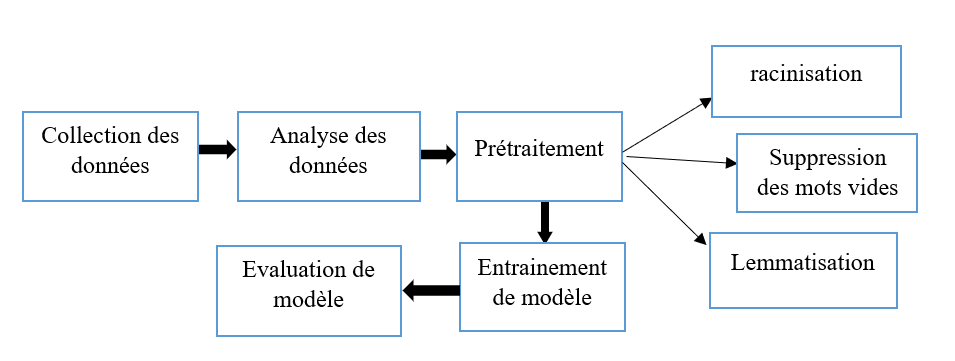
\includegraphics[width=0.9\textwidth]{project_report/figures/Capture d’écran (689).png} 
    \caption{\textit{Processus du traitement de langage naturel \cite{technoaretepublication}.}}
        \label{fig:figureProcess}
 
\end{figure}

%%%%%%%%%%%%%%%%%ù NLP APP %%%%%%%%%%%%%%%%%
\subsection{Domaine d'application}
Le traitement de langage naturel est le moteur de l’intelligence artificielle, avec des applications pratiques variées dans le monde actuel comme \cite{ibmNLP}:
\begin{itemize}
    \item \textbf{Traduction automatique:} Google Translate est un exemple couramment utilisé le traitement automatique de langage naturel (TALN). Une traduction efficace va au-delà du simple remplacement de mots d'une langue à une autre ; elle doit transmettre avec précision le sens et le ton du texte original dans la langue cible. La qualité des outils de traduction automatique s'améliore continuellement. Un bon test pour ces outils est de traduire un texte dans une autre langue, puis de le traduire à nouveau dans la langue d'origine. Par exemple, il y a quelques années, la phrase "The spirit is willing but the flesh is weak" traduite en russe puis en anglais donnait "The vodka is good but the meat is rotten." Aujourd'hui, la traduction inverse donne "The spirit desires, but the flesh is weak," montrant une amélioration notable, bien que ce ne soit pas encore parfait.
    \item \textbf{Agents virtuels et chatbots:} Les assistants virtuels comme Siri d'Apple et Alexa d'Amazon utilisent la reconnaissance vocale pour détecter des schémas dans les commandes vocales et la génération de langage naturel pour fournir des réponses appropriées. De même, les chatbots répondent aux textes saisis par les utilisateurs. Les meilleurs de ces systèmes apprennent à reconnaître des indices contextuels dans les demandes des utilisateurs, ce qui leur permet d'offrir des réponses de plus en plus pertinentes. Une prochaine avancée dans ce domaine est la réponse aux questions, où les systèmes pourront fournir des réponses pertinentes et utiles de manière proactive.
    \item \textbf{Résumé de texte:} Le résumé de texte emploie des techniques de TALN pour condenser de grands volumes de texte numérique en résumés ou synopsis. Cela est utile pour les index, les bases de données de recherche, ou pour les lecteurs pressés. Les meilleurs outils de résumé de texte utilisent le raisonnement sémantique et la génération de langage naturel pour ajouter du contexte et des conclusions pertinentes aux résumés.
\end{itemize}

%%%%%%%%%%%%%%%%%%%%ù APPROCHES %%%%%%%%%%%%%%
\section{Approches d'analyse des sentiments et des émotions}
L'analyse des sentiments repose sur plusieurs approches pour extraire et comprendre les émotions et les opinions dans un texte. Ces approches incluent (Voir la figure [\ref{fig:figure7}]): approche par lexique, approche hybride et approche basée sur le machine learning. Ces approches seront explorées en détail dans les sous-sections suivantes, mettant en lumière leurs avantages, leurs limitations et leurs applications spécifiques.

\begin{figure}[h]
    \centering
    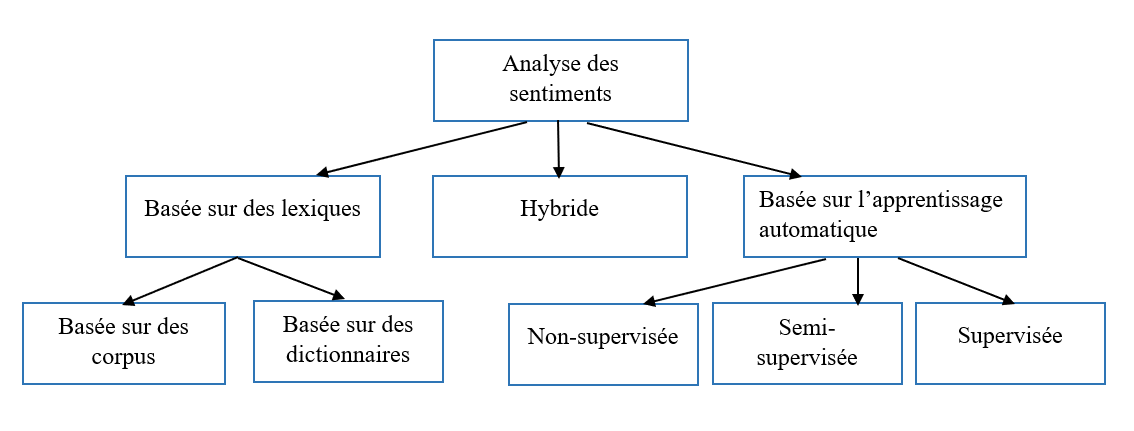
\includegraphics[width=1\textwidth]{project_report/figures/Capture d’écran (690).png} 
    \caption{\textit{Approches d'analyse des sentiments et des émotions }.}
        \label{fig:figure7}
 
\end{figure}

\subsection{Approche basée sur le machine learning}
L’approche de l’apprentissage automatique pour l’analyse des sentiments implique plusieurs étapes. Les données collectées à partir des diverses sources sont préretraitées en supprimant les mots vides pour l’élimination de bruit et la standardisation de format, les caractéristiques pertinentes sont alors extraites sous forme des vecteurs des mots à l’aide des techniques de représentation textuelle telles que le sac de mot ou TF-ID. Un algorithme de classification (régression logistique, les machines à vecteurs de support SVM, les réseaux de neurones...) choisi et entraîné sur l’ensemble des données, il apprend à associer certaines caractéristiques à des sentiments positifs, négatifs ou neutre et à des émotions de joie, de surprise, de peur..., afin d’être capable de classifier des nouveaux textes.  

%%%%%%%%%%%%%ùù LEXICAL APPROCHES %%%%%%%%%%
\subsection{Approche lexicale}
Une Méthode basée sur le lexique, elle repose sur l’utilisation des dictionnaires (Voir la figure [\ref{fig:figure7}], couramment utilisée en analyse des sentiments et dans l’autre application de NLP. \par
Un exemple populaire de modèle d'analyse de sentiment basé sur le lexique en Python est TextBlob. C’est une bibliothèque Python basée sur le Natural Language Toolkit (NLTK) qui calcule le score de sentiment pour les textes. Une technique de moyennage est appliquée à chaque mot pour obtenir les scores de polarité des sentiments pour l'ensemble du texte. \par
Les mots enregistrés dans le lexique de TextBlob ont leur score de polarité correspondant, score de subjectivité et score d'intensité. De plus, il peut y avoir différents enregistrements pour le même mot, donc le score de sentiment du mot est la valeur moyenne de la polarité de tous les enregistrements le contenant.

%%%%%%%%%%%%%ù HYBRIDE APPROCHE %%%%%%%%%%%
\subsection{Approche hybride}
L’approche hybride combine des méthodes basées sur le lexique (Voir la figure [\ref{fig:figure7}]) avec des techniques d’apprentissage automatique. Cette approche en analyse des sentiments permet d’obtenir des résultats plus précis et robustes en combinant les forces des méthodes basées sur le lexique et des techniques d’apprentissage automatique, elle offre une adaptabilité accrue et efficace pour le traitement des textes variés et complexes dans différents domaines.


%%%%%%%%%%%%%%%%%%ùù SENTIMENT ANALYSIS AND TWITTER %%%%
\section{L'analyse des sentiments et Twitter}





%%%%%%%%%%%%%%%%%%%%%% TWITTER %%%%%%%%%%%
\subsection{Twitter et ses attouts}
\textit{Twitter} fondé le 21 Mars 2006 et renommé \textit{X }en juillet 2023 est un réseau social de microbloguage, il permet aux utilisateurs de publier des messages courts qui ne dépassent pas 280 caractères (tweets), cette plateforme a connu une croissance régulière ces dernière années, est devenue un instrument incontournable de communication pour tous les acteurs sociaux (les hommes politiques, les sportifs, les dirigeants d’entreprise…) qui l’utilisent pour partager leurs actualités, leurs décisions, et leurs actions à venir. Twitter ou bien X constitue également une plateforme d’échange qui permet à tous d’exprimer son opinion en réaction à une annonce ou un événement, ce qui en fait un outil indispensable pour les personnes qui cherchent à comprendre les schémas de pensées des humaines.

%%%%%%%%%%%%%%%%%%%%% LATEST RESEARCH %%%%%%%%%%%%
\section{Travaux Connexes}
L'étude de l'analyse des sentiments est un domaine de recherche qui a suscité beaucoup d'intérêt. Les travaux antérieurs dans ce domaine se concentrent sur le développement des déverses méthodes et algorithmes pour classer les avis en catégorie telle que positive, négative, ou neutre. \par
La première approche était présentée par Hu et lui (2004), cette approche est basée sur l’analyse de la polarité pour classer les textes en fonctions de leur sentiment, l’objectif principal de hu et lui dans leur travail est de fournir aux consommateurs et aux entreprises des résumés utiles et des informations agrégées à partir des avis des clients afin de faciliter la prise de décision. Cette contribution à démontré aussi que l’incorporation des caractéristiques linguistiques spécifiques à Twitter (émoticônes, hashtags) pourrait améliorer les performances des modèles \cite{hu2004mining}. \par
Avec l’évolution des techniques d’apprentissage automatique, des algorithmes plus sophistiqués ont été appliqués. Par exemple Pak et Paroubek (2010) proposent différentes approches pour l’analyse des sentiments sur Twitter, alias X, des techniques de classification supervisée tels que Naïve Bayes et SVM et des méthodes basées sur l’apprentissage non supervisés (clustering) utilisés pour l’entraînement des modèles d’analyse de sentiments des tweets, Park et Paroubek évaluent également les performances de ces techniques, en mettant en lumière les caractéristiques uniques de Twitter et en proposant des approches pour relever les défis associés à l’analyse des sentiments sur cette plateforme \cite{pak2010twitter}. \par
De même, ils existent des marques, des entreprises et des organisations qu’ont un intérêt commercial auquel pourrait service un système autonome d’analyse des sentiments. L’étude menée par Rui, Liu et Whinston (2013) explore l’impact des tweets sur les ventes des billets de cinéma pour les films nouvellement sortis. Les résultats de cette étude ont montré que les tweets positifs étaient fortement corrélés avec une augmentation des ventes des billets de cinéma, tandis que les tweets négatifs avaient un effet dissuasif sur les ventes, ce qui suggère que la surveillance des sentiments sur Twitter peut fournir des indications précieuses sur les performances commerciales d’une entreprise \cite{rui2013whose}.  \par            
L’évolution de l’analyse des sentiments présente aussi ces dernières années un potentiel intéressant dans le domaine de la santé. Dans ce contexte, l’exploitation des données provenant de Twitter peut fournir des informations précieuses sur les expériences et les émotions des patients. Un exemple notable est l’étude menée par Crannell et Al (2016) sur le comportement d’utilisation de Twitter chez les survivants de cancer. Dans cette étude Crannell et Al ont collecté et analysé des tweets contenant des hashtags populaires liés au cancer. L’objectif principal était de comprendre les émotions dominantes exprimées chez les patients de cancer. Cette contribution a des implications importantes pour la communauté des patients et les organisations de la santé, car il met en évidence l’importance de soutien émotionnel sur le web. De plus, elle montre comment l’analyse des sentiments sur Twitter peut fournir des insights précieux pour comprendre les expériences des patients et améliorer les interventions de soutien \cite{crannell2016cancer}.

%%%%%%%%%%%%%%%%%% LIMITS  %%%%%%%%%%%%%%
\section{Défis et limitations d'analyse des sentiments et des émotions}
Malgré le progrès des technologies de langage de traitement automatique NLP, la compréhension de langage humaine est encore compliquée pour les machines:

%%%%%%%%%%%%%%%%%  SARCASME & IRONIE %%%%%%%%%%%%
\subsection{Sarcasme et Ironie}
Les expressions sarcastiques ou ironiques peuvent être difficiles à détecter par les modelés d’analyse des sentiments et des émotions, car ces expressions impliquent toujours un sens figuré ou inversé. Par exemple, « Bravo, tu as vraiment fait un travail formidable en oubliant de faire tes devoirs. »
Le modèle n’analyse pas la phrase avec une compréhension complète de scénario, il qualifiera l’expérience de positive sur la base de mots ‘Bravo’.  


%%%%%%%%%%%%%%%%%%%%%%ùù SUBJECTIVITE %%%%%%%%%%%%%%
\subsection{Subjectivité et Ambiguïté}
 L’analyse des sentiments peut rencontrer des difficultés avec des phrases subjectives et ambiguës. Les opinions et les sentiments exprimés sont parfois intrinsèquement subjectifs, ce qu’est perçu comme positif par une personne, peut être négatif par une autre. Par exemple, « le service était rapide mais impersonnel » peut refléter un sentiment mitigé ou équilibré en fonction des attentes et des critères de l’évaluateur. De même, le langage humain est souvent ambigu avec des phrases et des mots qui peuvent avoir plusieurs significations. Par exemple, « la présentation était intense » pourrait être interprétée positivement (comme une présentation intéressante) ou négativement (comme une présentation négative).     

 %%%%%%%%%%%%%%%%%%%%%%%%%%% MULTIPOLARITE %%%%%%%%%%
 \subsection{Multipolarité}
 La multipolarité consiste à identifier et à interpréter plusieurs sentiments contradictoires exprimés simultanément dans le même texte, elle présente un défi majeur pour les modèles d’analyse des sentiments. Un commentaire peut contenir des sentiments positifs et négatifs au même temps, par exemple « j’adore la qualité de caméra, mais la batterie est horrible », cette phrase contient deux opinions sur la qualité de produit (positive) et sur la batterie (négative), cette multipolarité rend l’analyse des sentiments plus complexe, car c’est difficile de distinguer à quelle classe le modèle doit ajouter cette phrase (positive, négative, ou neutre).
Ce qui nécessite des algorithmes avancés capable de traiter le contexte et de comprendre les nuances linguistiques.


%%%%%%%%%%%%%%%%%%%%%%%%%%%%% EVOLUTION DE LANGAGE %%%%
Le langage humain est une entité qui évolue rapidement et constamment, surtout dans le monde de web et des réseaux sociaux, des nouveaux mots, des expressions et des formes de communication émergent régulièrement, par exemple \textit{Twitter} ou bien \textit{X} voient naître des néologismes, des hashtags qui peuvent rapidement devenir des vecteurs importants d’opinions et d’émotions. Dans ce cadre, les modèles d’analyse des sentiments et de détection des émotions doivent être continuellement mis à jour pour intégrer ces nouveautés, non seulement par la collecte des nouvelles données, mais aussi par l’adaptation des nouveaux algorithmes de traitement. Jacob Eisenstein dans son article «\textit{ what to do about bad language on the internet} » écrit en 2023, souligne ce défi et propose des méthodes pour adapter les modèles aux changements linguistiques en temps réel \cite{eisenstein2013bad}.

\textbf{Conclusion}\par
En résumé, ce chapitre offre une plongée profonde dans le monde de l'analyse des sentiments et des émotions, mettant en lumière son rôle central dans notre société numérique moderne et explorant les opportunités et les défis qui l'accompagnent.







\clearpage
\chapter{MÉTHODE ET TECHNIQUES UTILISÉES POUR L'ANALYSE DES SENTIMENTS ET DES ÉMOTIONS}




\textbf{Introduction}\par
Ce chapitre se concentre sur les méthodes et techniques utilisées dans notre projet d'analyse des sentiments. Nous explorerons les approches spécifiques que nous avons adoptées pour extraire des informations significatives à partir de données textuelles, en mettant en lumière les outils et les modèles que nous avons utilisés pour analyser les opinions, les attitudes et les émotions exprimées dans le langage humain. En examinant ces méthodes, nous visons à fournir un aperçu clair et concis de notre approche d'analyse des sentiments, en soulignant les choix et les considérations qui ont guidé notre travail.



%%%%%%%%%%%%%%%%%%%%%%%%% CONTENUE %%%%%%%%%%%%%%%%

%%%%%%%%%%%%%%  COLLECTE DES DONNEES %%%%%%%%%%%%%%%%

\section{La collect des données}
La première étape du processus d'analyse des sentiments consiste à collecter des tweets en spécifiant un mot-clé pour récupérer tous les tweets liés à ce mot-clé. Les tweets peuvent être collectés à partir de différentes sources. L'un des moyens est le robot d'exploration de tweets qui collecte une collection de tweets liés en interrogeant le service Web Twitter ceci se voit nommé \textit{'Web Scraping'}. D’une autre façon en peut utiliser l'interface de programme d'application Twitter (API) \footnote{\href{https://developer.x.com/en/docs/twitter-api/v1/tweets/search/overview} {https://developer.x.com/en/docs/twitter-api/v1/tweets/search/overview}}. Cette API fournie par Twitter et qui donne aux développeurs la possibilité d'utiliser les fonctions de Twitter telles que la récupération de tweets avec le mot-clé et la langue sélectionné. Les tweets collectés seront stockés dans une base de données afin de les classer.

L'objectif le plus important de la collecte de données est de s'assurer que les données recueillies sont fiables et qu'elles regorgent d'informations intéressantes qui peuvent être analysées et transformées en décisions fondées sur des données \cite{questionpro}. 

\section{Exploration des données}
Une bonne connaissance de la santé des données permet d'améliorer la qualité de la fiabilité des informations. C'est à ce moment-là que l'exploration des données entre en jeu.\par
L'exploration des données fournit des informations détaillées sur les caractéristiques des données \cite{astera_blog}. Il s'agit d'identifier les types de données, les valeurs aberrantes, détecter les lignes dupliquées et traiter les données vides. Cet étape aide a comprendre les relations entre les variables et  les distributions des données afin de prendre des décisions éclairées. 

%%%%%%%%%%% PRETRAITEMENT %%%%%%%%%%%%%%%%%%%%%%%
\section{Le prétraitement}
Selon Flo Masdoum \cite{masdoum2023} , " La préparation des données est cruciale ! C'est un peu comme lorsqu'on plante des graines dans un jardin. Avant que les fleurs ne poussent, on prépare le sol et on élimine les mauvaises herbes. Le prétraitement des données dans le NLP, c'est la même idée, mais appliquée aux mots."


%%%%%%%%%%   NETTOYAGE %%%%%%%%%%
\subsection{Le nettoyages des données}
Le potentiel des données propres réside dans l’aisance de leur utilisation. Les données de qualité augmentent l’efficacité, que ce soit dans le cadre du projet pour lequel elles ont été collectées ou bien pour de futurs projets\cite{data_bird_blog}. Le processus de nettoyage des données est similaire pour la plupart des données, parfois il peut varier en fonction de la taille des ensembles de données, leurs nature et l'objectif de l'analyse. 
\subsubsection{Vérification du type des données}
Cet étape permet de vérifier que les ensembles de données ne contient qu’un unique type de données. Il permet d’identifier rapidement les valeurs aberrantes et les sources de problème \cite{data_bird_blog}. 
\subsubsection{ Gestion des valeurs manquantes}
Les valeurs manquantes peuvent entraîner une fausseté dans les résultats de l'analyse. Ils peuvent être traitées de différentes manières, telles que l'imputation par la moyenne, la médiane ou par des algorithmes plus complexes pour prédire les valeurs manquantes.
\subsubsection{Détection et correction des valeurs aberrantes}
Les valeurs aberrantes sont des valeurs extrêmes qui peuvent altérer les résultats de l'analyse. Comment les détecter et les corriger? Il est nécessaire de les repérer et d'évaluer afin de déterminer si elles nécessitent des corrections ou une suppression.
\subsubsection{Gestion des doublons}
Il se peut que lors de la collecte des données, certaines lignes apparaissent deux ou plusieurs fois, surtout lorsque l’on croise différentes sources. Les identifier et les supprimer dès le début permet de réduire le temps d’exécution de toutes les étapes du data cleaning \cite{data_bird_blog}.

%%%%%%%%% La conversion des données %%%%%%%%%
%%%%%%%%%%%% FIGURE %%%%%%%%%%%%%%%%%%%%%ùù
\subsection{Conversion des données}
\begin{figure}[h]
    \centering
    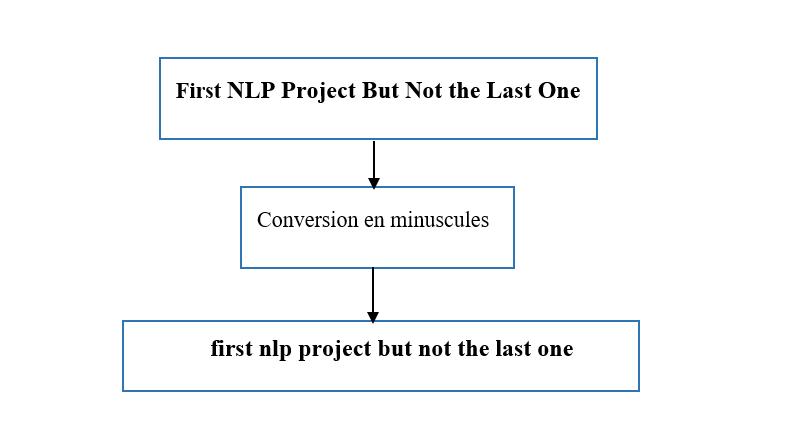
\includegraphics[width=0.7\textwidth]{project_report/figures/Capture d’écran (693).png} 
    \caption{\textit{Conversion des données en minuscules. }} 
    \label{fig:figureConver}
\end{figure}
%%%%%%%%%%%%%%%%%%%%%%%%%%%%%%%%%%%%%%%%%%%%%%%
Cet étape consiste a convertir les tweets en miniscules (Voir l'exemple dans la figure [\ref{fig:figureConver}] pour obtenir une base de données cohérente. Cela évite les problèmes liés à la case car les majuscules et les minuscules peuvent être interprétées différemment par les algorithms. Par exemple, "Hello" et "hello" seraient considérés comme deux mots différents, alors qu'ils devraient être traités comme le même mot. 



%%%%%%%%%%%% Tokenisation %%%%%%%%%%%%%%%%
\subsection{Tokenisation}
La tokenisation permet de décomposer une chaîne de caractères (message ou commentaire) en mots appelés \textit{Tokens }\footnote{un token peut être traduit en tant qu’unité lexicale.}.  Il est encore plus importante dans l’analyse des sentiments que dans d’autres domaines de la NLP, car les informations sur les sentiments sont souvent mal représentée \cite{singh2019nlp}. Cependant de nombreux cas ne sont pas triviaux à traiter \cite{coddity_nlp_blog} :
\begin{itemize}
    \item Les mots avec un trait d’union, exemple : peut être et peut-être qui ont des significations très différentes ;
    \item Les dates et heures qui peuvent être séparées par des points, des slashs, des deux points ;
    \item Les apostrophes ; 
    \item Les caractères spéciaux : émoticônes, formules mathématiques. 
\end{itemize}
La figure [\ref{fig:figureT}] suivante  un exemple de tokenisation, Le passage en minuscule est aussi 
intégré: 


%%%%%%%%%ù FIGURE %%%%%%%%%%%ùùù
\begin{figure}[h]
    \centering
    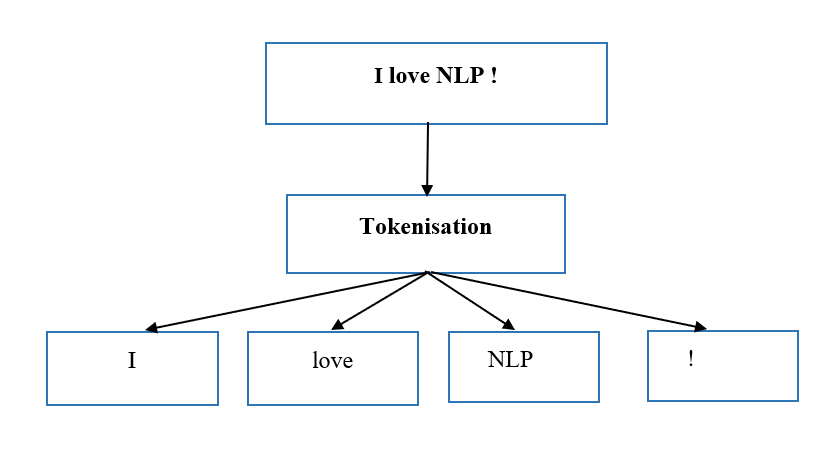
\includegraphics[width=1\textwidth]{project_report/figures/Capture d’écran (692).png} 
    \caption{\textit{Tokenisation}} 
    \label{fig:figureT}
\end{figure}

%%%%%%%%%%% SUPRESSION DES MOTS VIDES %%%%%%%%%%

\subsection{Supressions des mots vides ( StopWords)}
Les mots vides sont les mots qui n'ajoutent pas beaucoup de sens à une phrase. Ils peuvent être ignorés en toute sécurité sans sacrifier le sens de la phrase.  
En NLP, les mots comme "he", "this", "is" .. sont généralement supprimés du texte parce qu’ils peuvent causer du bruit et affecter la précision de l’analyse. Par exemple, Il existe de nombreuses bibliothèques qui fournissent des listes prédéfinies de mots vides dans différentes langues et qui peuvent être utilisées pour les supprimer du texte \cite{5degresNLP}. La figure suivante [\ref{fig:figureVIDE}] présente un exemple avant et après la suppression des mots vides:
%%%%%%%%%%%%%%%%% FIGURE %%%%%%%%%%%%%%%%%%%%
\begin{figure}[h]
    \centering
    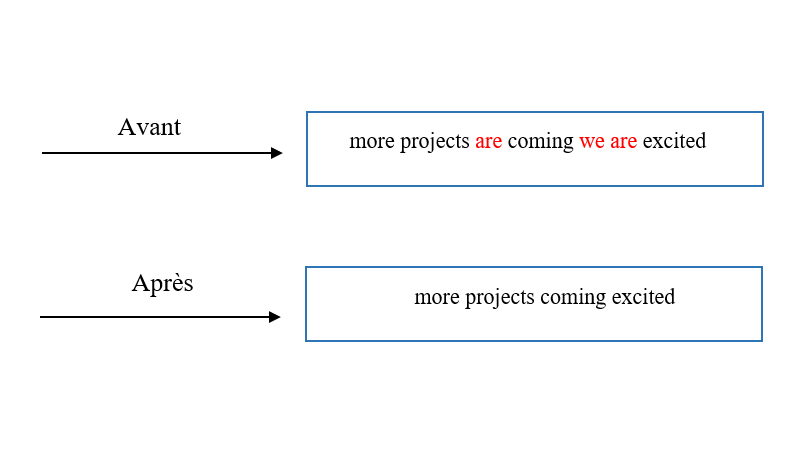
\includegraphics[width=0.7\textwidth]{project_report/figures/Capture d’écran (694).png} 
    \caption{\textit{Avant et après la suppression des mots vides. }} 
    \label{fig:figureVIDE}
\end{figure}

%%%%%%%%%%%%%%%%%%%%%%%%%%%ù


%%%%%%%%%%% GROUPEMENT SEMANTIQUE %%%%%%%%%%%%%
\subsection{Groupement Semantique}
En conséquence, une liste "nettoyée" de mots significatifs, séparés en tokens pour chaque document, est obtenue. Cependant, les mots peuvent être écrits au pluriel, au singulier, ou avec divers accords, tandis que les verbes peuvent être conjugués à différents temps et personnes.
Il est donc nécessaire de réduire les disparités grammaticales en identifiant des formes communes. Pour ce faire, deux approches différentes sont utilisées :
\begin{itemize}
    \item \textbf{La stemmatisation}, qui ignore l'environnement de la phrase. \hfill \\
    \item \textbf{La lemmatisation}, qui tient compte de la situation.
\end{itemize}


%%%%%%%%%%%%%%% Lemmatisation et stemming %%%%%%%%%%%

\subsection{ Stemming et Lemmatisation }
%%%%%%%%%%%%%%%%%%%ù FIGURE LIMMATISATION STEMMATISATION %%%%%

\begin{figure}[h]
    \centering
    \begin{minipage}{0.45\textwidth}
        \centering
        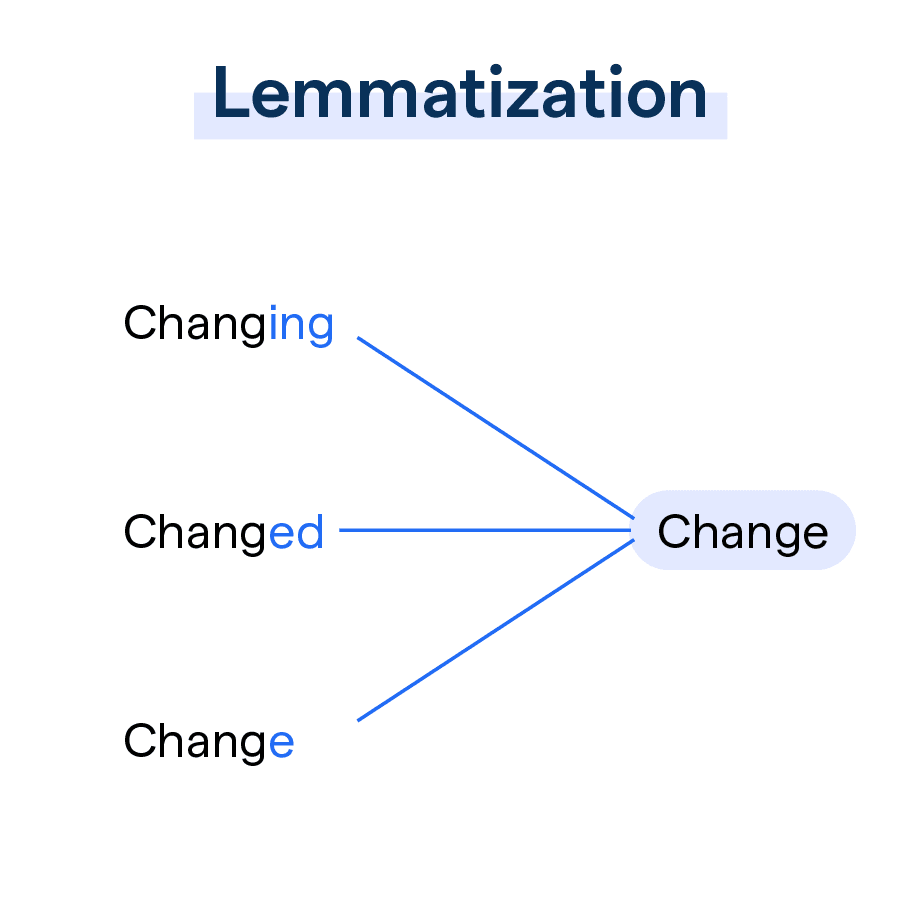
\includegraphics[width=\textwidth]{figures/Lemmatization_5338fc7c3e.png}
        \caption{\textit{Lemmatisation} \cite{botpenguinLemmatization}.}
        \label{fig:figureL}
    \end{minipage}\hfill
    \begin{minipage}{0.45\textwidth}
        \centering
        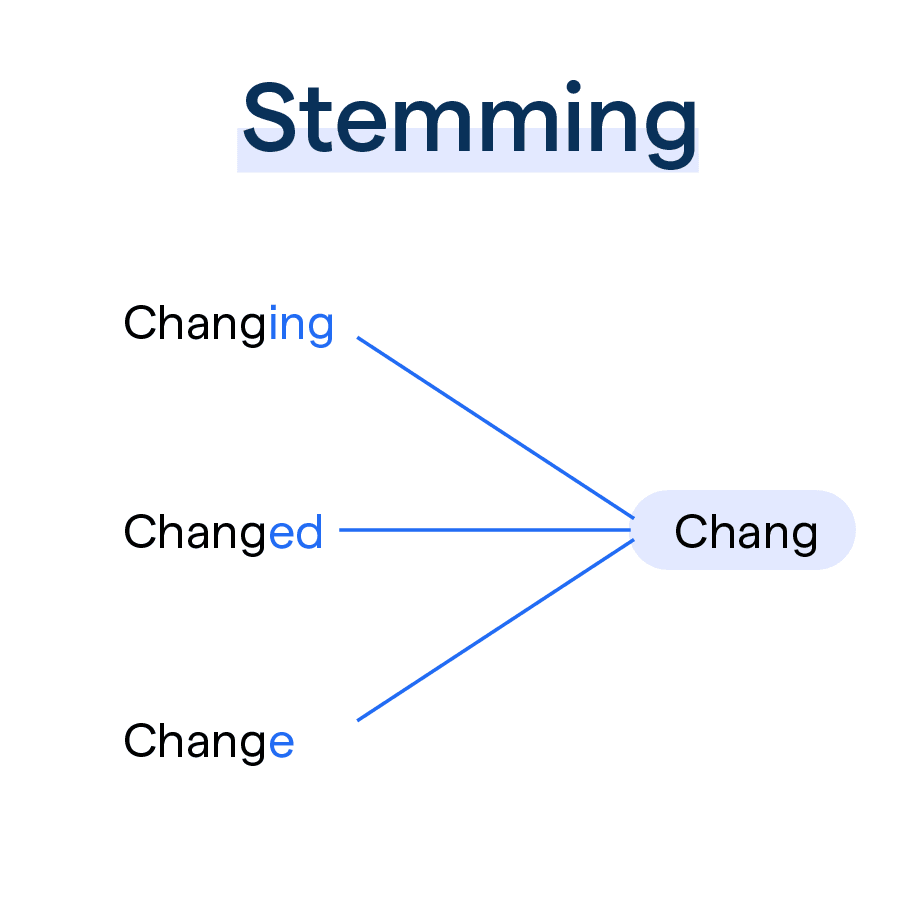
\includegraphics[width=\textwidth]{figures/Stemming_53678d43bc.png}
        \caption{\textit{Stemming }\cite{botpenguinLemmatization}.}
        \label{fig:figureS}
    \end{minipage}
\end{figure}

%%%%%%%%%%%%%%%%%%%%%%%%% TEXTE %%%%%%%%%%%%%%

La lemmatisation \cite{coddity_nlp_blog}, qui prend en considération le contexte dans lequel le mot est écrit, a pour but de trouver la forme canonique du mot, le lemme \footnote{Le lemme correspond à l’infinitif des verbes et à la forme au masculin singulier des noms, adjectifs et articles.}. Par conséquent, elle doit se faire après la transformation des lettres majuscules en minuscules et avant la tokenisation car les mots présents avant et après sont importants pour déterminer la nature du mot.
 Par exemple, cette méthode est capable de faire la différence entre “nous avions” : verbe avoir et “les avions”. \cite{coddity_nlp_blog}.

Le Stemming est  définit comme le processus qui génère des variantes d'un mot racine. En d'autres termes, il réduit un mot à sa forme de base. Cette méthode est utilisée pour simplifier la recherche et normaliser les phrases afin d'améliorer la compréhension (voir l'exemple dans la figure [\ref{fig:figureL}] et [\ref{fig:figureS}])
.
Le stemming et la lemmatisation ne sont pas toujours nécessaires ou bénéfiques pour chaque tâche NLP, et leur utilisation dépend de l’objectif, des données et du langage.




%%%%%%%%%%%%%%%% DIVISION DES DONNEES %%%%%%%%ù
\subsection{La division des données}
Cette étape consiste à séparer l'ensemble de données disponible en plusieurs sous-ensembles pour l'entraînement, la validation et le test des modèles. elle  permet d'évaluer de manière fiable les performances des modèles de machine learning et de deep learning, tout en garantissant qu'ils généralisent bien aux données non vues.

\begin{itemize}
    \item {\textbf{Entraînement :} La majorité des données (par exemple, 70 à 80 \%) est généralement utilisée pour entraîner le modèle. Pendant cette phase, le modèle apprend à partir des données et ajuste ses paramètres pour minimiser l'erreur.
    \item \textbf{Test :} Le reste des données (par exemple, 10 à 20 \%) est utilisé pour tester le modèle final. Ces données sont généralement utilisées une seule fois pour évaluer les performances du modèle après l'entraînement et la validation.}
\end{itemize}


En deep learning, il est généralement préférable de diviser les données en trois ensembles distincts : un ensemble d'entraînement, un ensemble de validation qui sert a évaluer les performances du modèle et un ensemble de test. Cette approche est souvent recommandée pour plusieurs raisons: 

\begin{itemize}
    \item \textbf{Optimisation des hyperparamètres :} En utilisant un ensemble de validation distinct, il est possible d'ajuster les hyperparamètres du modèle de manière plus efficace. Cela permet d'optimiser les performances du modèle sans risque de surajustement aux données d'entraînement.
   
    \item \textbf{Évaluation robuste :} La séparation des données en un ensemble de test distinct garantit une évaluation indépendante des performances du modèle sur des données réellement non vues. Cela permet d'estimer avec précision les performances du modèle dans des conditions réelles d'utilisation.
    
    \item \textbf{Prévention du surajustement :} En évaluant régulièrement les performances du modèle sur l'ensemble de validation pendant l'entraînement, il est possible de détecter et de prévenir le surajustement. Cela permet de garantir que le modèle généralise bien aux données non vues et qu'il n'apprend pas simplement les spécificités des données d'entraînement.
    
    \item \textbf{Comparaison des modèles : }En utilisant un ensemble de test distinct, il est possible de comparer les performances de plusieurs modèles de manière équitable. Cela permet de choisir le modèle le plus performant pour le déploiement en production.
\end{itemize}





%%%%%%%%%%%%%%%%%%%%% VALIDATION CROISEE %%%%%%%%%%%
\section{La validation coisée}
La validation croisée ( en anglais \textit{Cross validation)} est une technique importante en apprentissage automatique et en statistiques pour évaluer la performance d'un modèle et est particulièrement utile lorsque l'ensemble de données est limité. Au lieu de diviser les données en un ensemble de validation fixe et un ensemble de test, la validation croisée divise les données en plusieurs sous-ensembles (appelés "plis", \textit{en anglais "Folds"}) (voir la figure \ref{fig:figureVC}) et utilise chaque pli à tour de rôle comme ensemble de validation, tandis que les autres plis sont utilisés comme ensemble d'entraînement.\par

%%%%%%%%%%%%%%ùù FIGURE %%%%%%%%%%%%%%%%%ùùùù
\begin{figure}[h]
    \centering
    \includegraphics[width=0.7\textwidth]{project_report/figures/validation croisée.png} 
    \caption{\textit{Validation croisée} \cite{towardsdatascience_cross_validation}.}
        \label{fig:figureVC}
 
\end{figure}
%%%%%%%%%%%%%%%%%%% TEXTE %%%%%%%%%%%%%%%%%%ùùù
la validation croisée fonctionne comme la suite :

\begin{itemize}
    \item Division des données en k plis de taille égale (ou approximativement égale).
    \item Entraînement du modèle k fois, en utilisant chaque fois un pli différent comme ensemble de validation et les autres plis comme ensemble d'entraînement.
    \item Calcul de la performance du modèle sur chaque pli de validation et moyenne des performances pour obtenir une estimation globale de la performance du modèle.
\end{itemize}

%%%%%%%%%%%%%%%%%% FEATURE EXTRACTION %%%%%%%%%%

\section{Feature Extraction}

L'utilisation des données textuelles pour la modélisation prédictive, le texte doit être transformé en être utilisable par les algorithmes qui sont conçus pour travailler soit avec des entiers ou numéros réels. La transformation se compose de deux étapes: la tokenisation et la vectorisation.
La tokenisation se réfère à la division du texte en mots, ou tokens, qui représente l'unité atomique d'information. Le texte est donc vu comme une séquence de les jetons et l'étape suivante, la vectorisation, cartographie des jetons à une représentation numérique. Donc, avant d'utiliser les données, elles doivent être codées de manière appropriée. Chaque encodage
technique représente les données d'une manière différente et donc il peut influencer les performances des modèles. Le vecteur de comptage et le vecteur tf-idf ont été identifiés pour satisfaire ce besoin lorsqu'il s'agit de modèles traditionnels. De même, pour les modèles neuronaux, les données ont été encodées avec le vecteur TensorFlow.



%%%%%%%%%%%% BAG OF WORDS %%%%%%%%%%


\subsection{La méthode sac des mots (BagOfWords)}
Le "sac de mots" (ou "\textit{bag of words}" en anglais) est une représentation simplifiée d'un document en traitement automatique du langage naturel (NLP). Dans cette représentation, le texte est considéré comme un "sac" où l'ordre des mots est ignoré, seuls les mots et leur fréquence d'apparition sont pris en compte. \par 
Le principe du sac de mots est plutôt simple. Il se résume en 3 phases :
\begin{itemize}
    \item La décomposition des mots. On appelle cela aussi la tokenisation.
    \item La constitution d’un dictionnaire global qui sera en fait le vocabulaire.
    \item L’encodage des chaînes de caractère par rapport au vocabulaire constitué précédemment.
\end{itemize}

%%%%%%%%%%%%%% COUNT VICTORIZER %%%%%%%%%ù
\subsection{Encodage avec un vecteur de comptage (Count Vectorizer)}

%%%%%%%%%%%%%%%%%%%ùùù FIG %%%%%%%%%%%%%%%%%%%%%%%ùù
\begin{figure}[h]
    \centering
    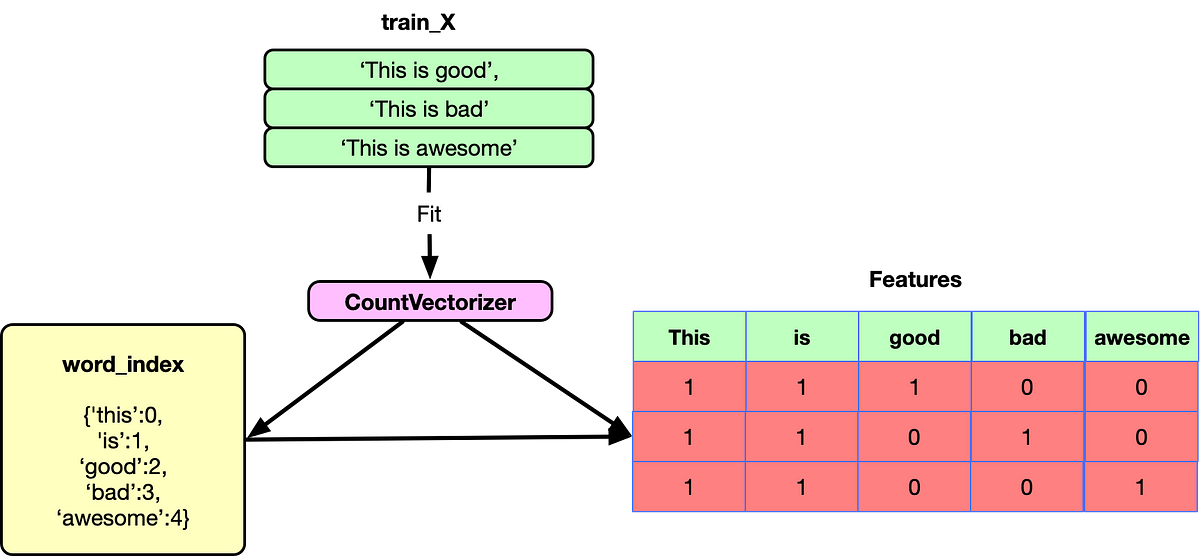
\includegraphics[width=0.7\textwidth]{project_report/figures/count vectorizer.png} 
    \caption{\textit{Vecteur de comptage (CountVectorizer)} \cite{shandeep92}.}
        \label{fig:figureCV}
 
\end{figure}
%%%%%%%%%%%%%%%%%%%%%%%%%%%%%%%%%%%%%%%%%%%%%%%%%

CountVectorizer est inclus dans la bibliothèque Scikit-learn\footnote{\href{https://scikit-learn.org/stable/}{https://scikit-learn.org/stable/}}. Il permet de convertir une série de documents textuels en une matrice de nombres de tokens (Voir l'exemple de la figure [\ref{fig:figureCV}]).  La nouvelle représentation des données présente un nombre de caractéristiques équivalent à la taille du vocabulaire déterminée par l'analyse des données.
En effet, les messages sont constitués de seulement quelques mots par rapport au nombre total de tokens, donc l'utilisation de matrices sparses permet de réduire considérablement la place nécessaire pour les stocker.
Il s'agit d'une méthode simple et basique qui ne prend pas en compte l'ordre des mots dans une phrase et l'importance de chaque mot.
Le CountVectorizer fonctionne comme la suite ( Voir la figure [\ref{fig:figureCV}]): 
\begin{enumerate}
    \item \textbf{Tokenisation :} Le CountVectorizer divise chaque document en mots ou en n-grammes. Un n-gramme est une séquence contiguë de n éléments dans le texte, généralement des mots.
   
    \item \textbf{Construction du vocabulaire :} Le CountVectorizer crée un vocabulaire unique en collectant tous les mots uniques dans l'ensemble des documents. Chaque mot devient une caractéristique dans l'espace vectoriel.
   
    \item \textbf{Création des vecteurs de comptage :} Pour chaque document, le CountVectorizer compte le nombre d'occurrences de chaque mot dans le vocabulaire. Chaque document est ensuite représenté par un vecteur où chaque élément correspond au nombre d'occurrences du mot correspondant dans ce document.
\end{enumerate}



%%%%%%%%%%%%% TF - IDF %%%%%%%%%%%%%%%%%%
\subsection{Encodage avec un vecteur TF-IDF}
Suivant l'idée qu'un mot qui se produit plusieurs fois est moins informatif dans les vecteurs codés que les autres mots qui se produisent moins souvent, une alternative à la vectorisation du nombre est de calculer les fréquences de mots. La méthode la plus populaire qui exploite cette approche est appelée « Fréquence de terme - fréquence inverse de document ». Chaque mot est attribué une valeur destinée à refléter l'importance de ce mot pour un document dans une collection de documents \cite{leskovec2014mining}. Cette valeur, appelée valeur tf-idf, est le produit de la fréquence du terme et de la Fréquence inverse du document.

En définissant $n_t$ comme le nombre de fois où le terme $t$ apparaît dans un document et Nt comme le nombre total de termes dans le document, la fréquence du terme t est définie comme suit :
\begin{equation}
\text{TF}(t) = \frac{n_t}{N_t}
\end{equation}
De la même manière, en définissant $N_d$ comme le nombre total de documents ou de messages dans le cadre de cette thèse, et en définissant $n_{d,t}$ comme le nombre de documents contenant le terme $t$, on peut définir la fréquence inverse des documents comme suit :
\begin{equation}  
\text{IDF}(t) = \log_e\left(\frac{N_d}{n_{d,t}}\right)
\end{equation}
La valeur finale n'est rien d'autre que le résultat de ces deux facteurs :
\begin{equation}
\text{TF-IDF}(t) = \text{TF}(t) \times \text{IDF}(t)
\end{equation}
Il augmente proportionnellement au nombre de fois qu'un mot apparaît dans le document et est contrebalancé par le nombre de documents dans le corpus contenant le mot, ce qui permet de s'adapter au fait que certains mots apparaissent plus fréquemment en général.


%%%%%%%%%%%%%%% N-GRAMMES %%%%%%%%%%%%%%%
\subsection{Encodage avec N-grammes}
L'encodage avec N-grammes dans le cadre du traitement du langage naturel (NLP) consiste à représenter un texte sous forme de séquences de mots contigus de longueur variable, au lieu de simplement considérer des mots individuels. Cette approche permet de capturer les relations entre les mots et le contexte dans lequel ils apparaissent. Il fonctionne comme la suite :

\begin{enumerate}
    \item \textbf{Définition des N-grammes :} Un N-gramme est une séquence de N mots consécutifs dans le texte. Par exemple, un bi-gramme est une paire de mots consécutifs, un tri-gramme est une séquence de trois mots, et ainsi de suite.
    
    \item \textbf{Création des N-grammes :} Pour créer des N-grammes, le texte est divisé en séquences de mots de longueur N. Par exemple, pour un texte "Le chat noir dort", les bi-grammes seraient ("Le", "chat"), ("chat", "noir"), ("noir", "dort"), etc.
    
    \item \textbf{Représentation sous forme de N-grammes :} Chaque N-gramme est ensuite représenté sous forme d'une unité distincte, souvent sous forme de vecteur ou de code numérique, qui capture la fréquence ou la présence de cette séquence dans le texte.
\end{enumerate}

%%%%%%%%%%%%%%%%%%% WORD EMBEDDING %%%%%%%%%%%
\subsection{Incorporation des mots ( Word Embedding)}
Dans son séminaire publié en 2017 pour les cours en ligne de l’université de Stanford, le professeur \textbf{\textit{Christopher Manning}} explique qu’au départ le fait de construire des modèles où les mots sont des éléments atomiques pose rapidement un problème dans le sens où leur représentation se fait via ce que l’on appelle de l’encodage one-hot où le lexique de mots est un long vecteur de 0 et le mot qui nous intéresse est le seul 1 du vecteur. Ceci pose donc un problème, surtout sachant que certains lexiques vocabulaires utilisés en apprentissage profond peuvent compter plusieurs millions de mots (plus de 13 millions de mots pour le Web 1T 5-gram39 corpus de Google par exemple). De plus, la nature atomique de ces représentations fait entièrement abstraction des relations entre les mots (par exemple les synonymes ou les équivalences de genre). Sachant cela, une solution possible consisterait à représenter les mots en tant que vecteurs dont les valeurs représentent d’autres mots qui ont un lien avec ceux-ci et qui sont eux aussi des vecteurs formatés de manière similaire (homme et femme pour reine et roi par exemple). C’est en se basant sur ce principe que l’on peut, via des bibliothèques de word embeddings comme word2vec40 ou GloVe41, construire de phrases composées de vecteurs contextuellement associables et utilisables dans les réseaux de neurones.

La représentation vectorielle est le point de départ de la transformation finale qui permet aux réseaux neuronaux d'apprendre des données d'entrée. On l'appelle l'emballage et il s'agit essentiellement d'une cartographie des données d'entrée sur un vecteur de nombres réels.
Le but des embellissements de mots est de capturer la signification sémantique, en la cartographiant dans un espace géométrique. Ceci est fait en associant un vecteur numérique à chaque mot dans un dictionnaire, de sorte que la distance entre deux vecteurs capturerait une partie de la relation sémantique entre les deux mots associés. L'espace géométrique formé par ces vecteurs est appelé un espace d'incorporation. Idéalement, dans un bon espace d'incorporation, les mots ayant une sémantique similaire sont placés à proximité l'un de l'autre dans l'espace, il est donc possible de classer le sentiment global d'une phrase, en analysant la représentation incrustée des mots qu'elle contient.
Keras offre un moyen simple de générer l'espace d'emballage. Cela se fait par l'intermédiaire de la couche d'intégration. Il prend comme entrée les séquences d'intégrales, qui ont été générées par la vectorisation, et produit la nouvelle représentation exploitée par les couches suivantes.

%%%%%%%%%%%%%%%%%%% MODELS %%%%%%%%%%%%%
\section{Approches basés sur Machine Learning }

%%%%%%%%%%%%%%%%%  REGRESSION %%%%%%%%%%%%%%%%%%%%%%ù
\subsection{Regression logistique}
La régression logistique est un modèle prédictif qui cherche à trouver des associations entre un
vecteur de variables explicatives aléatoires, de nature numérique ou catégorique, \( (x_1, x_2, \ldots, x_k) \),
et une variable dépendante catégorique binaire ou multinomiale \( Y \). Il s’agit tout simplement
d'une transformation non linéaire de la régression linéaire, où on cherche à prédire une classe à
la place d’une valeur numérique continue. Pour ce faire, on utilise une fonction logistique
appelée aussi 'Sigmoïde', pour retourner les probabilités qui sont utilisées pour séparer les
classes à prédire. Exemple : si la probabilité générée par une régression logistique, pour prédire
la tendance d’un titre, est supérieure à 0.5, alors la tendance prédite sera haussière, sinon, elle
est baissière.

Ce modèle produit une courbe logistique, qui est limitée aux valeurs comprises entre 0 et 1.
Soit :
\begin{itemize}
    \item \( Y \) la variable indépendante (à prédire),
    \item \( X = (X_1, X_2, \ldots, X_k) \) les variables dépendantes ou explicatives.
\end{itemize}

Comme le modèle est linéaire, on peut écrire l’équation de régression comme suit :
\[
Y^{(i)} = \beta_0 + \beta_1 x_1 + \beta_2 x_2 + \cdots + \beta_n x_n \quad \text{(3.5)}
\]

Les \( \beta_i \) sont les paramètres du modèle que nous cherchons à estimer pour obtenir notre fonction
de prédiction. On utilise le logarithme naturel des « cotes » de la variable dépendante pour
construire la courbe de la régression logistique, plutôt que la probabilité conditionnelle :
\[
\ln \left( \frac{p(Y = 1 \mid X)}{p(Y = 0 \mid X)} \right) = \beta_0 + \beta_1 x_1 + \beta_2 x_2 + \cdots + \beta_n x_n \quad \text{(3.6)}
\]

\[
p(Y = 1 \mid X) = \frac{e^{\beta_0 + \beta_1 x_1 + \beta_2 x_2 + \cdots + \beta_n x_n}}{1 + e^{\beta_0 + \beta_1 x_1 + \beta_2 x_2 + \cdots + \beta_n x_n}} = \frac{1}{1 + e^{-(\beta_0 + \beta_1 x_1 + \beta_2 x_2 + \cdots + \beta_n x_n)}} \quad \text{(3.7)}
\]


%%%%%%%%%%%% NAIVE BAYES %%%%%%%%%%%
\subsection{Naive Bayes}
Selon \cite{zhang2011novel}, Le classificateur Naive Bayes est l'un des algorithmes les plus puissants pour la classification, et il fonctionne bien même avec des millions d'entrées de données, étant rapide à former.\par
Naive Bayes \cite{konfuzio} est une méthode de classification probabiliste qui utilise le théorème de Bayes pour déterminer l'appartenance la plus probable des objets à une classe connue à l'aide de différentes propriétés. Ce principe peut être utilisé pour les modèles d'IA sous la forme de classificateurs Naive Bayes, qui distinguent par exemple les documents texte de manière algorithmique sur la base des mots qu'ils contiennent. Les propriétés ou caractéristiques qui renseignent l'algorithme sur l'appartenance à une classe sont appelées caractéristiques. Ces variables peuvent être continues, discrètes, catégorielles ou binaires, selon la nature des données d'entrée. \par

"Naïf", \cite{konfuzio} le processus l'est parce qu'il attribue aux caractéristiques une indépendance statistique les unes par rapport aux autres. Elles doivent en outre toutes contribuer dans la même mesure à la classification finale. Le théorème de Bayes, également connu sous le nom de théorème sous-jacent, a été établi par le mathématicien Thomas Bayes au 18e siècle. Il décrit une formule permettant de calculer la probabilité conditionnelle. En d'autres termes, il s'agit de déterminer la probabilité qu'un événement B se produise si l'événement A fait déjà partie de l'histoire. En termes mathématiques, cela se présente comme suit :

%%%%%%%%%%%%%%% THEOREME %%%%%%%%%%%%%%%%%%%%%%%%%%
\begin{theorem} 
Soient \( A \) et \( B \) deux événements, avec \( P(B) > 0 \). La probabilité conditionnelle de \( A \) sachant \( B \) est donnée par :
\[
P(A \mid B) = \frac{P(B \mid A) \, P(A)}{P(B)}
\]
où :
\begin{itemize}
    \item \( P(A \mid B) \) est la probabilité de \( A \) sachant que \( B \) est vrai.
    \item \( P(B \mid A) \) est la probabilité de \( B \) sachant que \( A \) est vrai.
    \item \( P(A) \) est la probabilité a priori de \( A \).
    \item \( P(B) \) est la probabilité a priori de \( B \).
\end{itemize}
\end{theorem}
\par

\subsubsection{Bayésien Naïf Multinomial}
Cette variante est surtout adaptée aux données d'entrée entières et suppose une distribution binomiale pour toutes les variables. Celle-ci décrit le nombre total de résultats positifs d'expériences de Bernoulli répétées. Pour les grands nombres, elle se rapproche de la distribution gaussienne, pour laquelle un type de classificateur spécifique peut être utilisé. L'expression multinomiale est souvent utilisée pour la classification de documents et de textes, où elle compte la fréquence des mots individuels \cite{konfuzio}.
\subsubsection{Bayésien Naïf Complémentaire}
Le modèle de Bayésien Naïf Complémentaire (BNC) est une variation améliorée du modèle de Bayésien Naïf classique, particulièrement adapté aux tâches de classification de texte. Contrairement au Bayésien Naïf traditionnel, qui repose sur une hypothèse d'indépendance forte entre les caractéristiques, le modèle de Bayésien Naïf Complémentaire tente de réduire les biais en tenant compte de l'influence complémentaire des autres classes.

\textbf{Principe et Fonctionnement:} \par
Le Bayésien Naïf Complémentaire se distingue en ajustant les probabilités pour mieux gérer les déséquilibres de classes et les caractéristiques corrélées. Il utilise les informations des autres classes pour améliorer la précision des prédictions, ce qui le rend particulièrement efficace dans des contextes où les classes sont inégales ou où les mots (caractéristiques) ont une forte corrélation.

\textbf{Parmi les avantages de ce modèle: }

\begin{itemize}
    \item \textbf{Meilleure gestion des déséquilibres de classes :} En tenant compte des informations provenant des classes complémentaires, le BNC réduit les biais introduits par les déséquilibres de classes.
    \item \textbf{Amélioration de la précision :} La prise en compte des influences complémentaires permet au modèle de faire des prédictions plus précises, en particulier dans les tâches de classification de texte.
    \item \textbf{Simplicité et efficacité :} Comme le Bayésien Naïf classique, le BNC est relativement simple à implémenter et à exécuter, tout en offrant des améliorations significatives en termes de performance.
    
\end{itemize}


%%%%%%%%%%%%%%  AdaBOOST %%%%%%%%%%%%%%%%%%%%%%
\subsection{AdaBoost}

\begin{figure}[h]
    \centering
    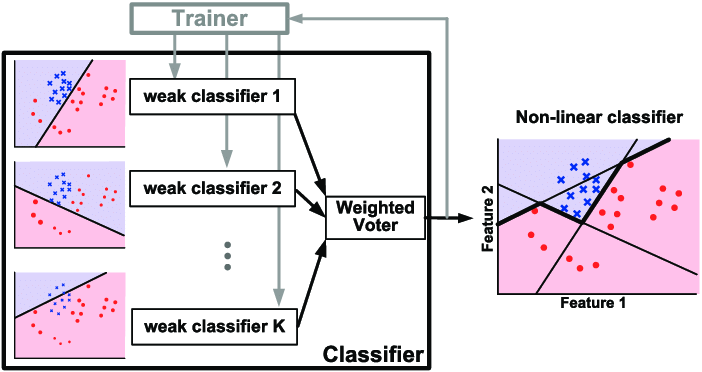
\includegraphics[width=0.7\textwidth]{project_report/figures/Illustration-of-AdaBoost-algorithm-for-creating-a-strong-classifier-based-on-multiple.png} 
    \caption{\textit{AdaBoost} \cite{researchgate2024}.}
        \label{fig:figure3}
 
\end{figure}

Le boosting adaptatif (AdaBoost) est l'un des premiers modèles de boosting\footnote{\href{https://aws.amazon.com/fr/what-is/boosting/}{https://aws.amazon.com/fr/what-is/boosting/}} développés. 
C'est \cite{fineproxy2024} une technique puissante utilisée dans l'apprentissage automatique et la science des données pour créer des algorithmes puissants qui améliorent les capacités prédictives. Il s'agit d'un algorithme de méta-apprentissage d'ensemble de type boosting itératif. L'objectif de l'algorithme AdaBoost est d'améliorer l'exactitude d'un modèle d'apprentissage faible et de créer un modèle amélioré et plus puissant.

AdaBoost fonctionne en combinant un ensemble de modèles faibles \textit{( 'Weak learners' en anglais}, ou "apprenants faibles"), en un seul modèle plus robuste. Chaque apprenant faible est formé sur différents aspects des données, et le modèle final est constitué des contributions de chacun d'entre eux ( Voir la figure \ref{fig:figure3}) . En utilisant plusieurs apprenants faibles, le modèle peut apprendre des modèles plus complexes dans les données qu'un seul apprenant fort ne peut le faire.\par

La clé d'AdaBoost est la sélection des apprenants faibles. Pour sélectionner la meilleure combinaison possible d'apprenants faibles, AdaBoost applique un système de pondération à chaque point de données. Le poids d'un point de données est augmenté s'il a été mal classé par un apprenant faible, et diminué s'il a été correctement classé. Ce système de pondération permet à AdaBoost de se concentrer sur les points de données les plus difficiles à classer et de former un meilleur modèle. \par

AdaBoost est utile pour les problèmes de classification, car il construit un modèle puissant qui peut classer avec précision des points de données, même avec des données bruitées ou incomplètes. AdaBoost est également utile pour les problèmes de régression, car il permet de réduire l'erreur quadratique moyenne en combinant les prédictions individuelles de l'apprenant faible.

\subsubsection{Description de l’algorithme AdaBoost}

Considérons un ensemble d’entraînement \( S = \{(x_1, y_1), \ldots, (x_n, y_n)\} \), où \( x_i \in X \) et \( y_i \in \{-1, 1\} \).

L’algorithme fonctionne comme suit :
\begin{enumerate}
    \item Initialiser les probabilités de chaque donnée \( p_1(i) = \frac{1}{N}, \; \forall \, i = 1, \ldots, N \)
    \item Entrainer le classifieur \( h_j \) avec \( X_j \). (généré à partir de \( X \) selon la probabilité \( p_j(i) \))
    \item Calculer l’erreur de \( h_j \) : \( \epsilon_j = \sum_{i=1}^{N} p_j(i) \delta(y_i \neq h_j(x_i)) \) \\
    (où \( \delta \) est une fonction indicatrice)
    \item Choisir un facteur \( \alpha_t = \frac{1}{2} \ln \left( \frac{1 - \epsilon_t}{\epsilon_t} \right) \)
    \item Mettre à jour la distribution des poids à travers des exemples :
    \[
    D_{t+1}(i) = \frac{D_t(i) \cdot e^{-\alpha_t y_i h_t(x_i)}}{Z_t}, \; \forall \, i \in \{1, 2, \ldots, m\}
    \]
    où \( Z_t \) est un facteur de normalisation.
\end{enumerate}

Résultat : la classe votée \( \forall \, x \), \( C(x) = \text{sign} \left( \sum_{t=1}^{T} \alpha_t \cdot f_t(x) \right) \)





%%%%%%%%%%%%%%%%%%% Nu-SVC %%%%%%%%%%%%%ù
\subsection{Nu-SVC}
Le nu-Support Vector Classification (nu-SVC) est une variante des Support Vector Machines (SVM)\footnote{\href{https://www.ibm.com/topics/support-vector-machine} {https://www.ibm.com/topics/support-vector-machine}}, un algorithme d'apprentissage supervisé largement utilisé pour la classification. Le nu-SVC utilise un paramètre de régularisation appelé "nu" au lieu du paramètre plus courant "C" utilisé dans les SVM traditionnels.

Le paramètre "nu" contrôle à la fois la marge du modèle et le taux d'erreurs tolérées lors de la classification. En d'autres termes, il détermine à la fois la largeur de la marge et le nombre d'erreurs de classification autorisées. Une valeur de "nu" plus basse indique une marge plus large et une tolérance plus élevée aux erreurs, tandis qu'une valeur plus élevée indique une marge plus étroite et une tolérance plus faible aux erreurs.

Le principal avantage du nu-SVC par rapport aux SVM traditionnels réside dans sa capacité à mieux gérer les données déséquilibrées, où les classes à prédire ont des proportions très différentes dans l'ensemble de données. En ajustant le paramètre "nu", le modèle peut être plus flexible dans la manière dont il traite les erreurs de classification, ce qui peut conduire à de meilleures performances dans de telles situations.

Le fonctionnement du nu-Support Vector Classification (nu-SVC) est similaire à celui des Support Vector Machines (SVM) traditionnels, avec une différence principale dans la façon dont il gère la régularisation: 

\begin{enumerate}
    \item \textbf{Séparation des données :} Comme les SVM traditionnels, le nu-SVC vise à trouver un hyperplan dans un espace de dimensions supérieures qui sépare les données en fonction de leurs étiquettes de classe. Cet hyperplan est choisi de manière à maximiser la marge, la distance entre l'hyperplan et les points de données les plus proches de chaque classe, appelés vecteurs de support.
   
    \item \textbf{Optimisation de la marge :} L'objectif est de trouver cet hyperplan de séparation tout en minimisant une fonction de coût. Dans le cas des SVM traditionnels, cette fonction de coût\footnote{La quantification de l'écart entre les prévisions du modèle et les observations réelles du jeu de donnée utilisé pendant l'entraînement} est généralement optimisée en ajustant le paramètre "C". Cependant, dans le nu-SVC, la régularisation est contrôlée par le paramètre "nu". Ce paramètre "nu" contrôle à la fois la largeur de la marge et le nombre d'erreurs de classification autorisées. Une valeur plus faible de "nu" correspond à une marge plus large et à une tolérance plus élevée aux erreurs, tandis qu'une valeur plus élevée de "nu" correspond à une marge plus étroite et à une tolérance plus faible aux erreurs.
   
    \item \textbf{Optimisation et entraînement :} Le modèle nu-SVC est entraîné à l'aide d'un algorithme d'optimisation qui ajuste les paramètres de l'hyperplan pour minimiser la fonction de coût, tout en tenant compte du paramètre "nu" spécifié par l'utilisateur. Cela implique souvent l'utilisation d'algorithmes d'optimisation tels que l'optimisation quadratique ou d'autres méthodes d'optimisation convexe.
   
    \item \textbf{Prédiction :} Une fois entraîné, le modèle nu-SVC peut être utilisé pour prédire les étiquettes de classe des nouveaux exemples en les classant par rapport à l'hyperplan de séparation trouvé pendant l'entraînement.
\end{enumerate}







%%%%%%%%%%%%%%%%% CNN %%%%%%%%%%%%%%%%%%%
\subsection{Les réseaux de neurones convolutif (CNN)}
Les réseaux de neurones convolutifs (également baptisés réseaux de neurones à convolution,\textit{ CNN }ou encore \textit{ConvNets}) sont une forme particulière de réseaux de neurones artificiels multicouches conçus pour traiter des données d’images bidimensionnelles bien qu’ils puissent être utilisés avec des données unidimensionnelles et tridimensionnelles \cite{lopez2020convolutional}. \par
L’architecture des connexions neurales de ces réseaux s’inspire de la structure du cortex visuel des mammifères \cite{lopez2020convolutional}. Ils sont composés de plusieurs couches de neurones combinées avec des fonctions mathématiques à plusieurs paramètres ajustables pouvant prétraiter une quantité d’informations restreinte, comme le montre la figure [\ref{fig:figure14}]:

%%%%%%%%%%%%%%%%%% FIG %%%%%%%%%%%%%%%%%%
\begin{figure}[h]
    \centering
    \includegraphics[width=0.7\textwidth]{project_report/figures/CNN modèle architecture (1).png} 
    \caption{\textit{Réseau de neurones convolutif} \cite{choudhry2024}.}
        \label{fig:figure14}
 
\end{figure}

Un réseau de neurones convolutif est caractérisé par une première couche dite « convolutionnelle » (généralement une à trois premières couches). Cette couche, comme son nom l’indique, est basée sur le principe mathématique de la convolution et tente d’identifier la présence d’un motif ou caractéristiques (par exemple dans une image ou un signal) \cite{lee2018convolutional}.
La convolution est une opération linéaire qui consiste simplement à appliquer un filtre, qui est une matrice bidimensionnelle de poids, à l’entrée du réseau, ce qui entraîne l’activation \cite{lee2018convolutional}. \par
L’application répétée du même filtre à l’entrée produit une carte d’activations appelée cartes des caractéristiques, qui montre la position et l’intensité des caractéristiques détectées dans l’entrées. Le filtre utilisé a une dimension plus petite que celle des données d’entrée. Ce filtre est multiplié via un produit scalaire par un bloc de l’entrée ayant la même tailles que le filtre \cite{lopez2020convolutional}. Le but de l’utilisation d’un filtre plus petit que l’entrée est parce qu’il permet au même filtre (matrice de poids) d’être multiplié par la matrice d’entrée (l’image) plusieurs fois à différents emplacements. Plus précisément, le filtre est systématiquement appliqué à chaque partie ou bloc des données d’entrés de la taille du filtre, de gauche à droite et de haut en bas. Une fois la carte des caractéristiques créée, chacune de ses valeurs peut alors être transférée par non-linéarité, comme la fonction ReLU, dont l’équation est la suivante \cite{lopez2020convolutional}:
\begin{equation}
f(x) = \max(0, x)
\end{equation}
pour tout réel \( x \). \par
L’application systématique d’un même filtre aux données d’entrée s’est avérée efficace : si le filtre est conçu pour détecter un certain type de caractéristiques sur l’entrée, l’application cohérente de ce filtre à l’ensemble de l’image d’entrée permet alors au filtre de détecter cette caractéristique où qu’elle soit sur l’image \cite{lopez2020convolutional}.

%%%%%%%%%%%%%% RNN %%%%%%%%%%%%%%%%
\subsection{Les réseaux de neurones réccurents (RNN)}
Les réseaux de neurones récurrents, également connus sous le nom de RNNs (pour Recurrent Neural Networks en anglais), sont un type de réseaux de neurones permettant aux prédictions antérieures d’être utilisées comme entrées via des états cachés (en anglais hidden states) \cite{wikiRNN}. Ceci est réalisé en propageant l’information dans les deux sens, y compris de couches cachées à la couche d’entrée. C’est ce mécanisme qui les rapproche du vrai fonctionnement du système nerveux, qui n’est pas à sens unique et qui les distingue des autres types de réseaux de neurones grâce à l’utilisation de boucles de rétraction pour traiter une séquence de données qui forme le résultat final, qui lui-même peut être une séquence de données \cite{wikiRNN}. Ces boucles de rétroaction rendent l’information durable, effet généralement équivalent à la mémoire. La figure [\ref{fig:figure1}] ci-dessous illustre une représentation d’un RNN :
%%%%%%%%%%%%%%%%%% FIG %%%%%%%%%%%%%%%%%%
\begin{figure}[h]
    \centering
    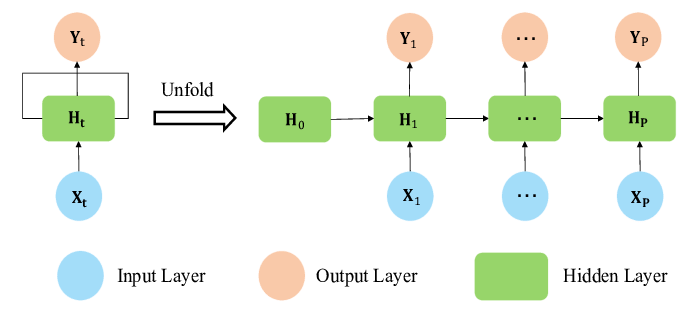
\includegraphics[width=0.7\textwidth]{project_report/figures/1_hpuxp7JFtcqysvkF_oJdRA.png} 
    \caption{\textit{Réseaux de neurones réccurents } \cite{choudhry2024}.}
        \label{fig:figure1}
 
\end{figure}

Le bloc étiqueté $A$ est un simple réseau de neurones à propagation directe déjà familier. Le côté droit de la figure montre le réseau $A$ à chaque pas de temps $t$, c’est-à-dire à $t = 0$, l’entrée $x_0$ est assimilée par le réseau pour générer la sortie $h_0$, l’entrée du pas de temps suivant est donc $x_1$. Seulement, il y a une entrée additionnelle du pas de temps précédent à partir du bloc $A$. Ainsi, le réseau neural prend en compte non seulement l’entrée actuelle, mais dispose aussi du contexte des entrées précédentes \cite{wikiRNN}. La figure suivante représente un échantillon du réseau neuronal récurrent, c’est-à-dire une unité unique du RNN :


Les formules régissant le calcul de la sortie d’une unité du RNN à l’instant \( t \) sont les suivantes \cite{wikiRNN}:
\begin{align}
A_t &= g(W_{ax} x_t + W_{aa} A_{t-1} + b_a) \\
h_t &= g(W_{ya} A_t + b_y)
\end{align}

Où :
\begin{itemize}
  \item \( A \) est la sortie de la couche cachée.
  \item \( g\)est la fonction d’activation.
  \item \( W \) est la matrice de poids.
  \item \( x \) est l’entrée.
  \item \( h \) est la sortie à un pas de temps \( t \).
  \item \( b \) est le biais.
\end{itemize}

Pour le RNN, la disparition du gradient est un problème majeur, puisque les réseaux de neurones qui ne peuvent plus être entrainés convenablement perdront inévitablement leurs performances. Cette disparition se produit dans les réseaux de neurones multicouches utilisés pour traiter des données complexes \cite{salehinejad2018recent}. Ajouter efficacement ces paramètres dès les premières couches nécessite beaucoup de temps et de ressources. Une façon de résoudre ce problème consiste en l’utilisations d’unités \textit{LSTM} \textit{(Long Short-Term Memory)} à mémoire court terme étendue. Les réseaux de neurones récurrents dotés d’unités LSTM sont capables de classer les données dans des cellules de mémoire à long terme ou à court terme. De cette manière, ils peuvent faire la distinction entre les données importantes devant être mémorisées et réinjectées dans le réseau et les données devant être « oubliées » \cite{salehinejad2018recent}.


%%%%%%%%%%%%%%% LSTM %%%%%%%%%

\section{Réseaux de neurones récurrents modernes(LSTM)}
Bien que les réseaux de neurones récurrents soient largement utilisés, ils ne sont pas suffisamment efficaces pour résoudre les problèmes actuels d'apprentissage de séquences. Par exemple, compte tenu de l'instabilité numérique lors du calcul du gradient, les réseaux de neurones modernes sont utilisés beaucoup plus souvent dans la pratique \cite{salehinejad2018recent}. \par
\subsection{Long Short-Term Memory (LSTM) }
%%%%%%%%%%%%%%%%%%%%ù FIG 

%%%%%%%%%%%%%%%%%%%%%%%%%%%%
Les cellules \textit{Long Short-Term Memory} sont conçues pour surmonter le problème de la disparition du gradient (en anglais,\textit{ Vanishing Gradient}) dans les réseaux de neurones récurrents et leur permettre de conserver les informations plus longtemps par rapport aux RNNs traditionnels \cite{hochreiter1997}. \par
Les LSTM ont la capacité de maintenir une erreur constante qui leur permet de continuer l’apprentissage sur de nombreux pas de temps et se propager à travers les couches \cite{hochreiter1997}.\par


Les LSTM disposent d’une structure en chaine qui contient quatre réseaux de neurones et différents blocs de mémoires appelés \textit{cellules}. Les informations sont sauvegardées par les cellules et les manipulations de la mémoire sont effectuées par ce qu’on appelle des « portes », qui sont des mécanismes internes permettant de réguler le flux d’information \cite{graves2012}, comme nous pouvons le constater dans l’architecture de la cellule LSTM représentée dans la figure ci-dessous :

%%%%%%%%%ù FIGURE %%%%%%%%%%%ùùù
\begin{figure}[h]
    \centering
    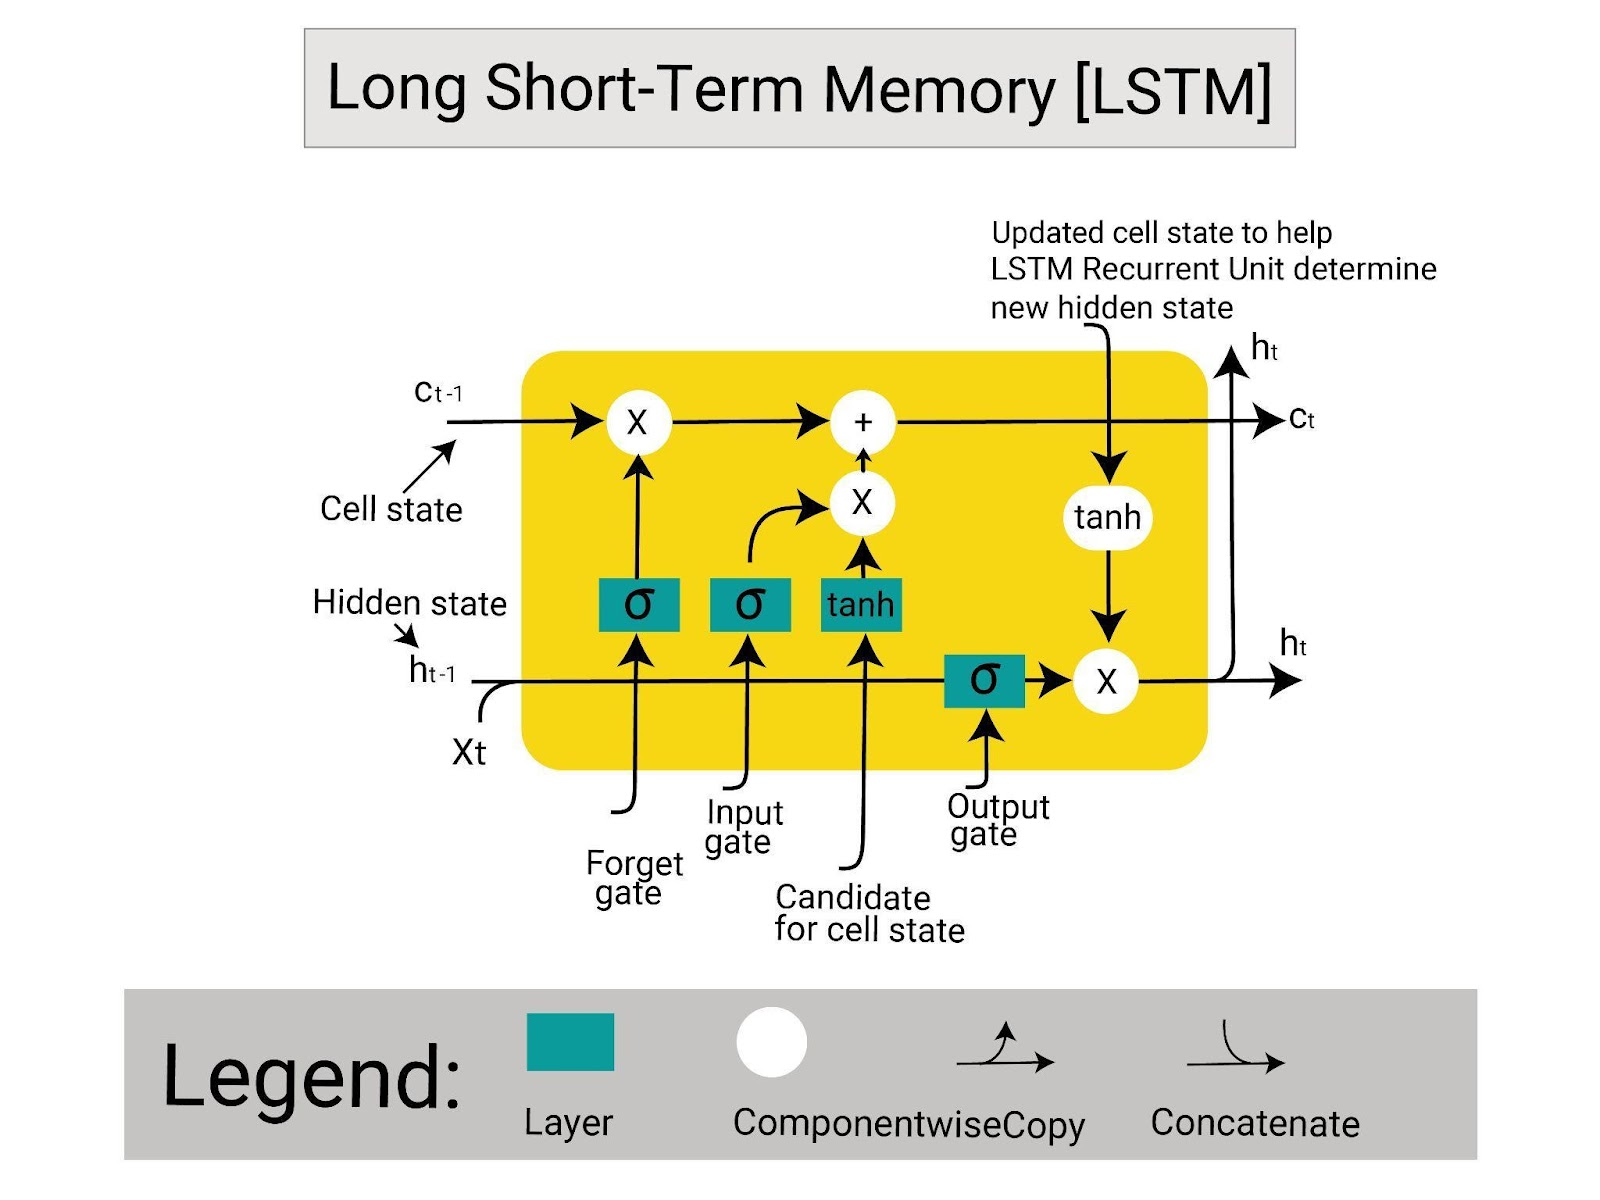
\includegraphics[width=0.7\textwidth]{project_report/figures/image-6.jpeg} 
    \caption{\textit{Long Short-Term Memory}  \cite{liberiangeek2024}.}
        \label{fig:figureLSTM}
 
\end{figure}



%%%%%%%%%%%%%%%%%% EVALUATION %%%%%%%%%%%%%%%
\section{Evaluation}
L'exactitude, la précision, le score F1 et le rappel sont des mesures communes pour mesurer les performances des modèles de classification.
Pour rappeler leur définition, il est utile d'introduire la matrice de confusion. C'est une matrice qui résume combien d'éléments d'entrée ont été correctement classés et combien n'en ont pas. Chaque ligne de la matrice représente les instances d'une classe prédite tandis que chaque colonne représente des instances dans une classe réelle. Les éléments classifiés relèvent des catégories suivantes :

\begin{itemize}
    \item Vrai Positive \textbf{(TP)} : nombre de tweets positifs classés correctement. \par
    \item Faux positive \textbf{(FP) }: nombre de tweets négatifs classés à tort comme positifs.\par
    \item Vrai Négative \textbf{(TN) }: nombre de tweets négatifs classés correctement.\par
    \item Faux Négative \textbf{(FN)} : nombre de tweets positifs classés à tort comme négatifs.\par
\end{itemize}


%% Table 



\begin{table}[h!]
    \centering
    \begin{tabular}{|c|c|c|}
        \hline
        & \multicolumn{2}{c|}{Classe Prédite} \\ \hline
        & Positif Prédit & Négatif Prédit \\ \hline
        Positif Réel & Vrai Positive (TP) & Faux Négative (FN) \\ \hline
        Négatif Réel & Faux Positif (FP) & Vrai Négatif (TN) \\ \hline
    \end{tabular}
    \caption{Matrice de confusion}
    \label{tab:confusion_matrix}
\end{table}
%%%%%%%  






%%%%%%%%%%%%%% PRECISION %%%%%%%%%%%%%%%%%%
\subsection{Précision}
La précision (\textit{Precision}) \cite{vilares2015lexicon} est également appelée valeur prédite positive, mesure la justesse
du modèle. Une précision plus élevée indique moins de FP. Mathématiquement, il est
défini comme : 
\begin{equation}
\text{Précision} = \frac{TP}{TP + FP}
\end{equation}
où :
\begin{itemize}
  \item $TP$ est le nombre de vrais positifs,
  \item $FP$ est le nombre de faux positifs.
\end{itemize}

%%%%%%%%%%%%%%% RAPPEL %%%%%%%%%%%%%
\subsection{Rappel}
Le rappel (\textit{Recall}) \cite{vilares2015lexicon}  est également connu sous le nom de sensibilité, mesure les cas positifs correctement classés par le modèle.  une valeur de rappel élevée signifie que peu de cas positifs sont mal classés comme négatifs. Le rappel peut être calculé à l'aide de la formule suivante: 

\begin{equation}
\text{Rappel} = \frac{TP}{TP + FN}
\end{equation}
où :
\begin{itemize}
  \item $TP$ est le nombre de vrais positifs,
  \item $FN$ est le nombre de faux négatifs.
\end{itemize}

%%%%%%%%%%%%%%%% EXACTITUDES %%%%%%%%%%%%%%%%%%%%
\subsection{Exactitudes}
L’exactitudes (\textit{Accuracy})  \cite{sebastiani2002text} utilisée comme mesure pour les techniques de catégorisation. Les valeurs de exactitudes, cependant, sont beaucoup moins réticentes aux variations du nombre de décisions correctes que la précision et le rappel. Cette technique est
représentée sous la forme suivante :
\begin{equation}
\text{Exactitude} = \frac{TP + TN}{TP + FP + TN + FN}
\end{equation}
où :
\begin{itemize}
  \item $TP$ est le nombre de vrais positifs,
  \item $TN$ est le nombre de vrais négatifs,
  \item $FP$ est le nombre de faux positifs,
  \item $FN$ est le nombre de faux négatifs.
\end{itemize}


%%%%%%%%%%%%%%%%%%%% F1 SCORE %%%%%%%%%%%ù
\subsection{Le score F1}
Le score F1 (\textit{F1-Score}) ou la mesure F1 \cite{vilares2015lexicon} est la moyenne harmonique de la précision et du rappel. Le score F peut être calculé comme suit :
\begin{equation}
\text{Score F1} = 2 \times \frac{\text{Précision} \times \text{Rappel}}{\text{Précision} + \text{Rappel}}
\end{equation}
où :
\begin{itemize}
  \item $\text{Précision}$ est la précision,
  \item $\text{Rappel}$ est le rappel.
\end{itemize}
\vspace{0.5cm}
\textbf{Conclusion}\\
En conclusion, ce chapitre a mis en lumière les méthodes et techniques clés utilisées dans notre projet. Des modèles d'apprentissage automatique avancés aux méthodes de prétraitement textuel, nous avons exploré une gamme diversifiée d'approches visant à capturer la richesse et la complexité des données textuelles. Ces méthodes et techniques, combinées à une compréhension approfondie du domaine et des besoins spécifiques de notre projet, ont permis d'obtenir des résultats prometteurs dans l'analyse des sentiments.







\clearpage
\chapter{IMPLEMENTATION ET RESULTATS}

\textbf{Introduction}\par
Ce chapitre se concentre sur l'implémentation des résultats de notre projet, en mettant en lumière les performances des modèles et les résultats obtenus à partir de nos expériences. Nous présenterons une analyse détaillée des performances de chaque modèle utilisé, en mettant en évidence les forces et les faiblesses de chacun. En outre, nous effectuerons une comparaison approfondie des résultats obtenus, en examinant les métriques de performance clés telles que la précision, le rappel et la F-mesure. Cette section offrira un aperçu complet des résultats de notre projet d'analyse des sentiments, en fournissant des informations précieuses sur l'efficacité de nos approches et sur les leçons apprises tout au long du processus d'implémentation.

\section{Environement de travail et les outils }
\subsection{Langague de programmation}
Nous avons utilisé le langage de programmation\textbf{\textit{ Python}} comme principal outil de développement en raison de sa syntaxe simple et lisible, son caractère open source qui lui confère une utilisation libre, ses riches bibliothèques spécialisés comme ScikitLearn, les outils interactifs comme Jupyter Notebooks facilitant l’expérimentation et le prototypage rapide.
Python se démarque comme un choix idéal pour le déploiement des modèles d’apprentissage automatique d’une manière efficace car il permet aux développeurs de se focaliser sur leurs taches plutôt que sur les détails de mis en œuvre.      

\subsection{Environnement de développement}

%%%%%%%%%%%%% JUPYTER %%%%%%%%%%
\subsubsection{Jupyter Notebook}
Le langage de programmation Python est utilisé dans de plusieurs IDE. Pour ce projet nous avons choisi l'IDE Jupyter Notebook,  étant une application web open source et qui est utilisée pour créer et partager des documents contenant du code, des équations, des visualisations et du texte. \par
Dans le cadre de l'installation de Jupyter, nous avons opté pour la distribution Anaconda. Cette distribution propose un ensemble d'outils particulièrement pertinents pour les Data Scientists, qui leur permettent de tirer pleinement parti de la puissance impressionnante de Python. Outre sa gratuité et son caractère open source, Anaconda simplifie le processus de travail grâce à son accessibilité accrue. L'installation des bibliothèques dans l'environnement Anaconda suffit pour les rendre opérationnelles et pour coder sur Jupyter. \par
Les packages contenus dans la distribution Anaconda sont compatibles avec Windows, Linux et MacOS. Parmi les packages les plus populaires et couramment employés, on retrouve numpy, scipy, sklearn, keras, TensorFlow, opencv, matplotlib, entre autres. Au cours de ce projet, nous avons principalement travaillé avec les trois derniers packages mentionnés.
%%%%%%%%%%%%%%%%%%%% VS CODE %%%%%%%%%%%%
\subsubsection{Visual Studio Code }
Pour la programmation de l’interface web on a utilisé Visual Studio Code, souvent abrégé VS Code, qu’est un éditeur de code source gratuit et open-source développé par Microsoft. Il est largement utilisé par les développeurs de logiciels pour la programmation, l'édition et le débogage de code. VS Code offre de nombreuses fonctionnalités avancées telles que la coloration syntaxique, la complétion automatique, l'intégration avec des systèmes de contrôle de version, des extensions personnalisables, et bien plus encore. Il est disponible sur différentes plateformes, y compris Windows, MacOs et Linux, ce qui en fait un choix populaire pour les développeurs travaillant sur une variété de langages de programmation

%%%%%%%%%%%%%%%%%%%%%%%%ù BIBIOTHEQUES %%%%%%%%%%%

\subsection{Bibliothèques utilisées}


 \textbf{NUMPY}\footnote{\href{https://numpy.org/}{https://numpy.org/}} est la bibliothèque open-source fondamentale du calcul scientifique en Python pour le traitement de tableaux à usage général (voir le logo dans la figure ci- dessous). Elle fournit des tableaux multidimensionnels de haute performance et des outils pour les manipuler. \par
 Au-delà de ses nombreuses utilisations dans le cadre scientifique, Numpy peut aussi être utilisée en tant que conteneur multidimensionnel performant pour des données générales. Ce qui rend NumPy accessible et productif est sa syntaxe de haut niveau, sa large variété de fonctions mathématiques complètes et de générateurs de nombres aléatoires ainsi que sa capacité de prise en charge d’un large éventail de plateformes matérielles et informatiques. 
 \par
 
\textbf{PANDAS}
\footnote{\href{https://pandas.pydata.org/}{https://pandas.pydata.org/}} est une bibliothèque open source de Python, largement utilisée pour la manipulation et l'analyse de données. Développée initialement par Wes McKinney en 2008, Pandas offre des structures de données flexibles et expressives, principalement les DataFrames et les Series, permettant des opérations rapides et faciles sur des ensembles de données tabulaires et des séries chronologiques. \par

\textbf{MATPLOTLIB} \footnote{\href{https://matplotlib.org/}{https://matplotlib.org/}} est une bibliothèque de visualisation de données en Python qui offre une vaste gamme de graphiques pour représenter visuellement des données. Créée par John D. Hunter en 2003, Matplotlib est particulièrement prisée pour sa capacité à générer des graphiques statiques, animés et interactifs de haute qualité.\par

\textbf{SEABORN}\footnote{\href{https://seaborn.pydata.org/}{https://seaborn.pydata.org/}} est une bibliothèque de visualisation de données basée sur Matplotlib. Elle est conçue pour rendre les graphiques statistiques plus attrayants et plus faciles à créer. Seaborn simplifie la création de visualisations complexes et est particulièrement bien adaptée pour travailler avec des données structurées comme les DataFrames de Pandas.\par 

\textbf{NLTK}\footnote{\href{https://www.nltk.org/}{https://www.nltk.org/}} (Natural Language ToolKit) est une collection de modules de programmes open-source, de didacticiels et d’ensembles de problèmes permettant de créer des programmes pour l’analyse de texte. Ce kit a été à l’origine créé par Steven Bird et Edward Loper en conjonction avec des cours de linguistique computationnelle à l’université de Pennsylvanie en 2001.\par
NLTK inclut le traitement statistique du langage naturel et est lié à des corpus labélisés. Joint à la librairie, NTLK offre des tutoriels, des échantillons de données, des démonstrations graphiques ainsi qu’une documentation complète sur l’interface de programmation API.\par


\textbf{Scikit-learn}, souvent abrégé en "sklearn", est une bibliothèque open source en Python spécialisée dans le domaine de l'apprentissage automatique (machine Learning). Elle propose une large gamme d'algorithmes et d'outils pour la création, l'entraînement et l'évaluation de modèles de machine Learning. Cette bibliothèque vise à rendre l'apprentissage automatique plus accessible grâce à des interfaces conviviales et cohérentes.
Scikit-learn est reconnue pour sa simplicité et sa modularité. Elle couvre différents types d'apprentissage, tels que la classification, la régression, le regroupement (clustering), la réduction de dimension, la détection d'anomalies, et bien plus encore. Elle propose une grande variété d'algorithmes populaires, notamment les machines à vecteurs de support (SVM), les forêts aléatoires, les k-plus proches voisins (KNN), la régression linéaire, et bien d'autres.
En outre, scikit-learn fournit des outils pour la préparation des données, l'évaluation des performances des modèles et la validation croisée. Cette bibliothèque est largement utilisée par les professionnels du machine learning en raison de sa documentation complète, de sa grande communauté et de son intégration aisée avec d'autres bibliothèques Python telles que Numpy, pandas et matplotlib.

\textbf{TensorFlow} \footnote{\href{https://www.tensorflow.org/?hl=fr}{https://www.tensorflow.org/?hl=fr}} est une plateforme d’apprentissage automatique open source de bout en bout (voir le logo dans la figure ci-dessous). Il est doté d’un écosystème exhaustif et flexible de bibliothèques, de ressources et d’outils communautaires permettant aux chercheurs de promouvoir les avancées de l’apprentissage automatique, et aux développeurs de créer et de déployer aisément des applications d’apprentissage automatique.\par
 TensorFlow a vu le jour aux mains d’ingénieurs et de chercheurs membres de l’équipe Google Brain au sein de l’organisation de recherche sur l’intelligence artificielle de Google. TensorFlow fournit des API Python et C++ statistiques, ainsi qu’une API rétro compatible non cautionnée pour d’autres langages. \par

\textbf{Keras} \footnote{\href{https://keras.io/}{https://keras.io/}}  est une bibliothèque de haut niveau pour le développement et l'entraînement de modèles de réseaux de neurones profonds. Initialement développée par François Chollet, Keras est maintenant intégrée au sein de la bibliothèque TensorFlow de Google, mais elle peut également être utilisée avec d'autres backends comme Theano ou CNTK. \par

\textbf{Djanjo}\footnote{\href{https://www.djangoproject.com/}{https://www.djangoproject.com/}} est un framework web de haut niveau écrit en Python qui permet le développement rapide et facile de sites web robustes et sécurisés. Créé par Adrian Holovaty et Simon Willison en 2003, Django est conçu pour aider les développeurs à prendre des applications du concept à la réalisation aussi rapidement que possible.

%%%%%%%% Présentation DES CORPUS %%%%%%%%%%%%%%%%
\section{Présentation des corpus} 
Les ensembles de données utilisées dans ce projet ont été extraits de Kaggle \footnote{\href{https://www.kaggle.com/} {https://www.kaggle.com/}}.  La plateforme fournit des jeux de données, des notebooks et des didacticiels gratuits dont les scientifiques de données ont besoin pour réaliser leurs projets d'apprentissage automatique \cite{kaggle_wiki}. 

%%%%%%%%%%%%%%%ù SENTIMENTs DATA %%%%%%%%%%%%%%%
\subsection{Sentiment140-MV }
Le dataset des sentiments également connu sous le nom  \textit{Sentiment140-MV} \footnote{\href{https://www.kaggle.com/datasets/kamyab20/sentiment140mv} {https://www.kaggle.com/datasets/kamyab20/sentiment140mv}}, est un ensemble de données largement utilisé dans le domaine de l'analyse des sentiments. Il comprend des tweets collectés à partir de Twitter, annotés avec l'étiquette du sentiment correspondant, généralement positif et négatif.  
Chaque entrée de données a les caractéristiques suivantes :
\begin{itemize}
    \item {\textbf{ Ids:}} un nombre entier qui représente l'id du tweet;
    \item {\textbf{Date:}} le timestamp du tweet; \par
    \item {\textbf{ Flag:}}  la requête qui a été utilisée pour récupérer le Tweet avec Twitter API. S'il n'y a pas de requête, cette valeur est NO QUERY. 
    \item {\textbf{Utilisateur:}} le nom de l’utilisateur qui a publié le message;
    \item {\textbf{ texte:}} le contenu réel du tweet.
\end{itemize}

La figure [\ref{fig:figure8}]  montre l'apparence du jeu de données Sentiment140-MV avant toute opération supplémentaire effectuée sur celui-ci.


\begin{figure}[h]
    \centering
    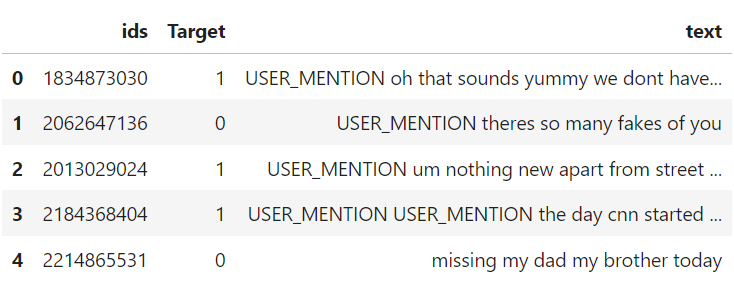
\includegraphics[width=0.7\textwidth]{project_report/figures/Dataset-APRES.png} 
    \caption{Sentiment140-MV dataset originale. }
        \label{fig:figure8}
 
\end{figure}

%%%%%%%%%%%%%%%% EMOTIONS DATA %%%%%%%%%%%%%%%%
\subsection{Emotions}
Le dataset \textit{Emotions}\footnote{\href{https://www.kaggle.com/datasets/nelgiriyewithana/emotions} {https://www.kaggle.com/datasets/nelgiriyewithana/emotions}} est une collection de messages en anglais provenant de Twitter, minutieusement annotés avec six émotions fondamentales: la colère, la peur, la joie, l'amour, la tristesse et la surprise. Ce dataset constitue une ressource précieuse pour comprendre et analyser le spectre diversifié des émotions exprimées dans les textes courts sur les réseaux sociaux. Chaque entrée dans ce dataset se compose d'un segment de texte représentant un message Twitter et d'une étiquette correspondante indiquant l'émotion prédominante transmise. Les émotions sont classées en six catégories : la tristesse (0), la joie (1), l'amour (2), la colère (3), la peur (4) et la surprise (5).

La figure [\ref{fig:figEm}]  montre l'apparence du jeu de données Emotionq avant toute opération supplémentaire effectuée sur celui-ci.

\begin{figure}[h]
    \centering
    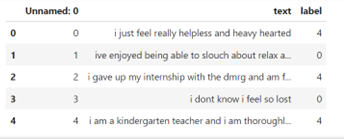
\includegraphics[width=0.7\linewidth]{project_report/figures/emotion.png}
    \caption{Emotions dataset originale.}
    \label{fig:figEm}
\end{figure}




Une analyse descriptive a été effectuée pour mieux comprendre les ensembles de données et obtenez des informations à ce sujet. Il est rapporté dans la section suivante avec une analyse exploratoire des données et quelques astuces de pré-traitement pour réduire le bruit des données.




%%%%%%%%%%%%%%%%%ù ANALYSE DES SENTIMENTS %%%%%%%%
\section{Analyse des sentiments}
Un flux précis a été suivi pour exécuter les expériences, afin d'éviter d'introduire \textit{Bias} dus à des exécutions non structurées. À partir de l'ensemble de données brut, les données
ont été pré-traitées en supprimant les hashtags, les mentions, les ponctuations et les mots d'arrêt, pour réduire les données non informatives, réduisant ainsi la taille globale des données pour gérer, accélérer les expériences.  toutes les lettres et les mots sont changés en lettres de cas inférieures \textit{(Lower-case)} pour assurer l'uniformité. En outre, les phrases ont été divisées en mots individuels, ou des jetons en utilisant le Tokeniser de NLTK. 
le processus est le même pour tout nos modules. Chaque séquence des deux corpus passe par les mêmes étapes de prétraitement.  

%%%%%%%%%%%%%%%%%%% ANALYSE EXPLORATOIRE %%%%%%%%%%%%%

\subsection{Analyse éxploratoire}


\begin{figure}[h]
    \centering
    \includegraphics[width=0.6\linewidth]{project_report/figures/WhatsApp Image 2024-06-07 à 20.42.44_c32b6e6d.jpg}
    \caption{Distribution des classes dans l'ensemble des données Sentiment140-MV.}
    \label{fig:figDes}
\end{figure}

%%%%%%%%%%%%%%%%%%%%%%%%%%%%%%%%%%%%%%%%%%%%%%%%%%%%%
19 995 messages étiquetés sont disponibles, ils sont soit positifs soit négatifs et les deux classes ne  sont pas équilibrées comme le montre l figure [\ref{fig:figDes}]. Cela a été fait exprès par les créateurs du jeu de données pour limiter les complexités liées aux classes déséquilibrées, ce qui simplifie ainsi les phases suivantes. 




%%%%%%%%%%%%%%%%%%%%%%%%%%%%%%%%%%%%%%%%%%%%%%%%%
%%%%%%%%%%%%%% Statistique du dataset %%%%%%%%%%%



\begin{table}[h!]
    \centering
    \begin{tabular}{>{\raggedright\arraybackslash}p{0.6\linewidth}>{\centering\arraybackslash}p{0.3\linewidth}}
        \textbf{Statistique} & \textbf{Valeur} \\
        Nombre moyen de caractères : & 73 \\
        \multicolumn{2}{c}{\rule{0.8\linewidth}{0.4pt}} \\
        Tweet le plus long : & 157 caractères \\
        \multicolumn{2}{c}{\rule{0.8\linewidth}{0.4pt}} \\
        Tweet le plus court : & 3 caractères \\
        \multicolumn{2}{c}{\rule{0.8\linewidth}{0.4pt}} \\
        Nombre de caractères, quantile 0,99 : & 134 \\
        \multicolumn{2}{c}{\rule{0.8\linewidth}{0.4pt}} \\
        Nombre moyen de mots : & 14 \\
        \multicolumn{2}{c}{\rule{0.8\linewidth}{0.4pt}} \\
        Tweet le plus long : & 33 mots \\
        \multicolumn{2}{c}{\rule{0.8\linewidth}{0.4pt}} \\
        Tweet le plus court: & 1 mot \\
        \multicolumn{2}{c}{\rule{0.8\linewidth}{0.4pt}} \\
        Nombre de mots, quantile 0,99 : & 28 \\
        \multicolumn{2}{c}{\rule{0.8\linewidth}{0.4pt}} \\
        Nombre de mots uniques : & 18835 \\
    \end{tabular}
    \caption{Statistiques du jeu de données}
    \label{tab:dataset_statistics}
\end{table}
%%%%%%%%%%%%%%%%%%%%%%%%%%%%%%%%%%%%%%%%%%%%%%%%%%%ù

Pour comprendre l'effet du pré-traitement, une analyse quantitative a été réalisée avant de prendre toute mesure sur le corpus. Les statistiques clés concernant la longueur des Tweets sont résumées ici dans le tableau [\ref{tab:dataset_statistics}]. 

%%%%%%%%%%%%%%%%%%%%%%%% PRE-TRAITEMENT %%%%%%%%%%%



\subsection{Nettoyage des données} 
Dans la phase de nettoyage des données, un processus rigoureux a été entrepris pour garantir la qualité et la cohérence du jeu de données. Tout d'abord, les lignes en double ont été identifiées et éliminées, permettant ainsi d'assurer l'intégrité des enregistrements. De plus, dans le souci de ne conserver que les informations essentielles pour l'analyse ultérieure, seules les colonnes pertinentes ont été préservées. Parmi celles-ci figuraient les identifiants uniques associés à chaque entrée, la variable cible indiquant la polarité sentimentale (positif ou négatif), ainsi que le texte brut des messages eux-mêmes. Cette approche sélective a non seulement simplifié le jeu de données, mais a également facilité les étapes suivantes d'analyse et de modélisation.
%%%%%%%%%%%%%%% TABLE %%%%%%%%%%%%%%%%ùù
\begin{table}[h!]
    \centering
    \begin{tabular}{lll}
        \toprule
        \textbf{Variable} & \textbf{Avant nettoyage} & \textbf{Après nettoyage} \\
        \midrule
        Nombre d'entrées & 19995 & 18213 \\
        Nombre de colonnes & 6 & 3 \\
        Types de données & \texttt{int64 (2), object (1)} & \texttt{int64 (4), object (2)} \\
        Doublons & 1782 & - \\
        \midrule
        \textbf{Cible} & & \\
        Positif & 11628 & - \\
        Négatif & 6585 & - \\
        \bottomrule
    \end{tabular}
    \caption{Caractéristiques du jeu de données avant et après le nettoyage}
    \label{tab:data_summary}
\end{table}
Le tableau [\ref{tab:data_summary}] fournit un résumé des données avant et après le processus de nettoyage, mettant en évidence le nombre d'enregistrements avant le nettoyage ainsi que le nombre de lignes dupliquées identifiées.


\newpage

%%%%%%%%%%%%%%%%%%%%%%%%%%%%%%%
\subsection{Préparation des données}
Au cours de prétraitement des données, nous avons utilisé deux méthodes : lemmatisation et le stemming, la première consiste à réduire les mots à leurs formes de base en utilisant des règles heuristiques simple, tandis que la deuxième utilise des règles linguistiques pour transformer les mots en leurs lemme correct.
L’utilisation des deux méthodes a produit des résultats similaires, ce qui s’explique par le contexte limité du dataset des sentiments avec peu de variations morphologiques et grammatical, par conséquence les transformations nécessaires pour réduire ces formes sont minimales.

\subsection{Représentation textuelle}
%%%%%%%%%%%%%%%%%%%ù TABLE %%%%%%%%%%%%%%%%%%%%%%
\begin{table}[h!]
    \centering
    \begin{tabular}{lcccccccc}
        \toprule
        & \multicolumn{4}{c}{CountVectorizer} \\
        \cmidrule(lr){2-5}
        Métriques & Accuracy & Précision & Recall & F1-score \\
        \midrule
        RL & 89\% & 90\% & 93\% & 91\% \\
        CNB & 85\% & 89\% & 87\% & 88\% \\
        MNB & 84\% & 85\% & 91\% & 88\% \\
        \bottomrule
    \end{tabular}
    \caption{Performances des modèles avec CountVectorizer}
    \label{tab:model_performance_countvectorizer}
\end{table}

\begin{table}[h!]
    \centering
    \begin{tabular}{lcccccccc}
        \toprule
        & \multicolumn{4}{c}{TF-IDF vectorizer} \\
        \cmidrule(lr){2-5}
        Métriques & Accuracy & Précision & Recall & F1-score \\
        \midrule
        RL & 87\% & 87\% & 94\% & 90\% \\
        CNB & 84\% & 86\% & 89\% & 88\% \\
        MNB & 78\% & 75\% & 98\% & 85\% \\
        \bottomrule
    \end{tabular}
    \caption{Performances des modèles avec TF-IDF vectorizer}
    \label{tab:model_performance_tfidfvectorizer}
\end{table}

Pour la représentation textuelle, deux méthodes ont été introduites ; TF-IDF et     CountVectorizer. Cette dernière est la méthode la plus simple pour créer des vecteurs, elle compte le nombre des mots dans un document, Il ne prend pas en compte l'importance relative des mots dans le corpus. En revanche TF-IDF (Term Frequency-Inverse Document Frequency) prend en compte à la fois la fréquence des termes dans un document (TF) et l'inverse de la fréquence des documents dans lesquels un terme apparaît (IDF)
Pour l’analyse préliminaire des données, nous avons utilisé la régression logistique, la naïve Bayes multinomial et la naïve Bayes complément comme algorithmes de base en raison de leur simplicité, de leur rapidité et aussi leurs faibles besoins en calcul.
TF-IDF a donné des résultats moins performants que CountVectorizer, cela peut être dû à   la simplicité et l’efficacité de comptage brut des occurrences qui semble mieux s’adapter avec les caractéristiques spécifiques de ce dataset.







 
%%%%%%%%%% DIVISION DES DONNEES %%%%%%%%%%%%%%%%%
\subsection{Division des données}
Dans cette étape, nous avons procédé à la division des données en ensembles d'entraînement, de validation et de test, en suivant une approche adaptée à chaque type de modèle : les modèles de machine learning et les modèles de deep learning.

Pour les modèles de machine learning traditionnels, tels que les SVM, Naive Bayes et Régression Logistique, nous avons simplement divisé les données en un ensemble d'entraînement et un ensemble de test. L'ensemble d'entraînement a été utilisé pour entraîner le modèle, tandis que l'ensemble de test a été réservé pour évaluer la performance du modèle final sur des données non vues.

Pour les modèles de deep learning, en raison de leur complexité et de leur tendance à sur-ajuster aux données, nous avons effectué une division plus fine en trois ensembles : un ensemble d'entraînement, un ensemble de validation et un ensemble de test. L'ensemble d'entraînement a été utilisé pour entraîner le modèle, l'ensemble de validation a été utilisé pour ajuster les hyperparamètres et surveiller la performance pendant l'entraînement, et l'ensemble de test a été utilisé pour évaluer la performance finale du modèle sur des données non vues.

Les deux tableaux suivants présentent les résultats obtenus lors de la division des données en différentes tailles pour les modèles de régression logistique et de complément naïf bayésien. 

%%%%%%%%%%%%%%%%%%%%%% TABLE %%%%%%%%%%%%%%%%%%%
\begin{table}[h!]
    \centering
    \caption{\textit{Performances du modèle RL}}
    \begin{tabular}{lcccc}
        \toprule
        Test\_size & Accuracy & Recall & Précision & F1\_score \\
        \midrule
        0.1 & 0.87 & 0.94 & 0.86 & 0.90 \\
        0.2 & 0.87 & 0.94 & 0.87 & 0.90 \\
        0.3 & 0.86 & 0.94 & 0.86 & 0.90 \\
        0.4 & 0.87 & 0.94 & 0.86 & 0.89 \\
        \bottomrule
    \end{tabular}
\end{table}

\begin{table}[h!]
    \centering
    \caption{\textit{Performance du modèle CNB}}
    \begin{tabular}{lcccc}
        \toprule
        Test\_size & Accuracy & Recall & Précision & F1\_score \\
        \midrule
        0.1 & 0.87 & 0.94 & 0.86 & 0.90 \\
        0.2 & 0.85 & 0.87 & 0.89 & 0.88 \\
        0.3 & 0.86 & 0.94 & 0.86 & 0.90 \\
        0.4 & 0.87 & 0.94 & 0.86 & 0.89 \\
        \bottomrule
    \end{tabular}
\end{table} 
\newpage

Dans la lumière de ces résultats, on observe que peu de changements significatifs sont remarqués dans les performances des modèles, ce qui suggère que la division des données en différentes tailles de test n'a pas un impact considérable sur les performances des modèles de régression logistique et de complément naïf bayésien. Cela indique une certaine robustesse des modèles par rapport à la variation de la taille des données de test. Il est également important de noter que, malgré les légères fluctuations observées dans les métriques de performance telles que l'accuracy, le recall, la précision et le F1-score, les performances générales des modèles restent relativement stables sur différentes divisions des données. Ces résultats sont encourageants car ils suggèrent que les modèles sont capables de généraliser efficacement sur de nouveaux ensembles de données, ce qui est essentiel pour assurer leur utilité dans des applications réelles. Cependant, il convient de poursuivre l'exploration de ces modèles sur d'autres jeux de données et de considérer d'autres facteurs pouvant influencer leurs performances, tels que la qualité et la quantité des données d'entraînement.


%%%%%%%%%%% CLASSIFICATION %%%%%%%%%%%% 
\subsection{La classification}
Pour cette tâche d’analyse des sentiments et de classification en positive et négative sur le jeu de données sentiment140-MV, nous avons utilisé des algorithmes d’apprentissage automatique supervisé tels que :
\begin{itemize}
    \item Régression logistique
    \item Naïve Bayes multinomial
    \item Naïve Bayes complément
    \item Adaboost
    \item NuSVC
    \item RNN-LSTM
\end{itemize}

La performance des modelés créés à l’aide de ces classificateurs est évaluée en calculant l’accuracy, la précision, le recall, et le F1-score, ainsi en visualisant la matrice de confusion et les graphiques de performance pour les réseaux de neurones.   
%%%%%%%%%%%%%%%%%%%%%% RESULTATS %%%%%%%

\subsection{Résultats et discussion }
%%%%%%%%%%%%%%%%%%%%%%%%%% TABLE %%%%%%%%%%%
\begin{table}[h!]
    \centering
    \begin{tabular}{lcccc}
        \toprule
        \textbf{Classificateur} & \textbf{Accuracy} & \textbf{Precision} & \textbf{Recall} & \textbf{F1-score} \\
        \midrule
        Model 1 : RNN\_LSTM & 85\% & 85\% & 85\% & 85\% \\
        Modèle 2 : MNB & 78\% & 82\% & 78\% & 85\% \\
        Modèle 3 : CNB & 85\% & 85\% & 85\% & - \\
        Modèle 4 : RL & 87\% & 88\% & 88\% & 87\% \\
        Modèle 5 : AdaBoost & 80\% & 81\% & 80\% & 81\% \\
        Model 6 : Nu-SVC & 87\% & 88\% & 88\% & 88\% \\
        \bottomrule
    \end{tabular}
    \caption{Performance des classificateurs}
    \label{tab:classifier_performance}
\end{table}

%%%%%%%%%%%%%%%%%%%%%%%%%%%%%%%%%%%%%%%%%%%%%
Le modele Naïve Bayes multinomial est moins performant en comparaison avec les autres modèles ; bien que le MNB soit simple et rapide à entrainer, il suppose l’indépendance conditionnelle entre les caractéristiques ce qui n’est pas entièrement applicable aux données textuelles, aussi il est moins performant sur les datasets ou les classes sont déséquilibrés parce qu’il est basé sur le fréquence brute dans les calculs des probabilités. \par
\begin{figure}[h]
    \centering
    \begin{minipage}{0.45\textwidth}
        \centering
        \includegraphics[width=0.8\textwidth]{project_report/figures/complementNB_sentimentçmatrice.png}
        \caption{\textit{Matrice de confusion du modèle CNB}.}
        \label{fig:figureSHJJJR}
    \end{minipage}\hfill
    \begin{minipage}{0.45\textwidth}
        \centering
        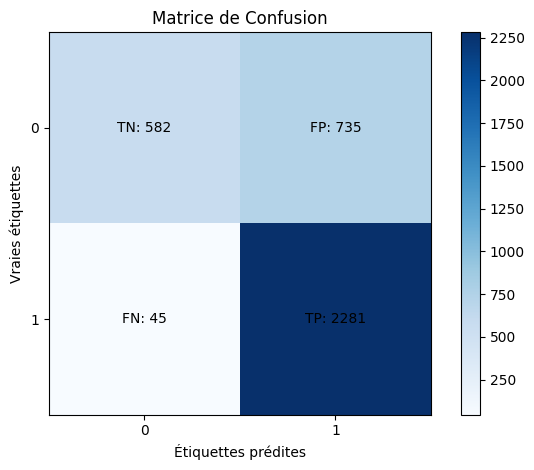
\includegraphics[width=0.8\textwidth]{project_report/figures/multinomial NB_sentiment_matrice.png}
        \caption{\textit{Matrice de confusion du modèle MNB }.}
        \label{fig:figureNBVV}
    \end{minipage}
\end{figure} 


Concernant le modele Naïve Bayes complément est parmi les algorithmes les plus performant sur ce dataset des sentiments en notant sa rapidité, cela s’explique par le fait CNB est performant sur les jeux donnés déséquilibrés comme dans notre cas où il fonctionne en ajustant la manière dont les probabilités sont calculées pour tenir compte des données manquants par rapport à d’autre classes (basé sur la fréquence complément).\par
\begin{figure}[h]
    \centering
    \begin{minipage}{0.45\textwidth}
        \centering
        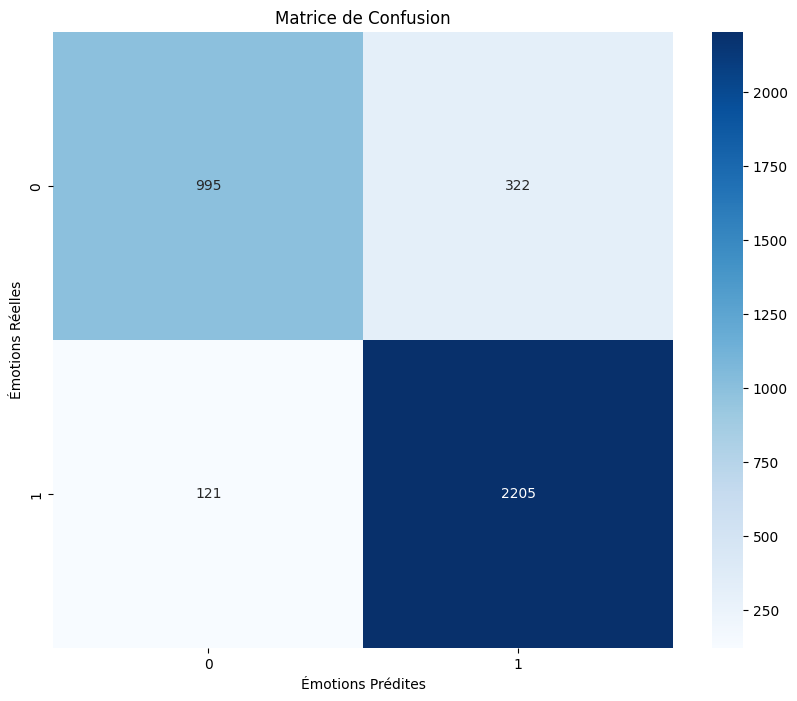
\includegraphics[width=0.8\textwidth]{project_report/figures/matrice_sentimnt-NUSVC.png}
        \caption{\textit{Matrice de confusion du modèle nu-SVC}.}
        \label{fig:figureSHJJJR}
    \end{minipage}\hfill
    \begin{minipage}{0.45\textwidth}
        \centering
        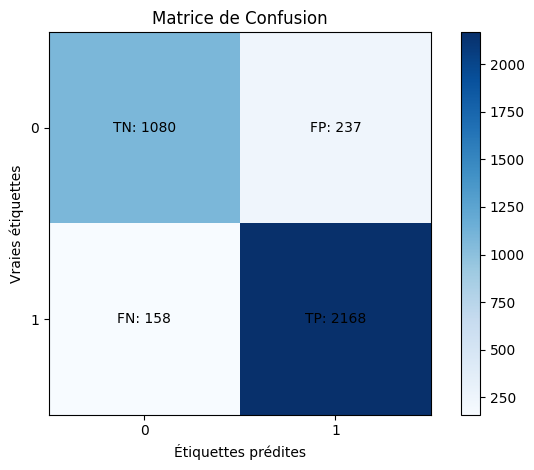
\includegraphics[width=0.8\textwidth]{project_report/figures/RL_sentiment_matrice.png}
        \caption{\textit{Matrice de confusion du modèle RL }.}
        \label{fig:figureNBVV}
    \end{minipage}
\end{figure} 
Pour NuSVC et la régression logistique, ces modèles ont réussi à capturer efficacement les relations entre les caractéristiques des données et des classes des sentiments leurs efficacité peut être attribuée à leur capacité à modéliser des frontières de décision complexes tout en maintenant une interprétabilité raisonnable ce qui en fait des choix attrayants pour les applications de classifications.\par
\begin{figure}[h]
    \centering
    \begin{minipage}{0.45\textwidth}
        \centering
        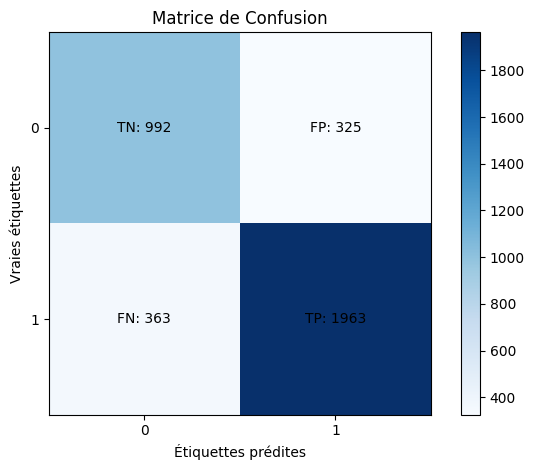
\includegraphics[width=0.8\textwidth]{project_report/figures/adaboost_sentiment_matrice.png}
        \caption{\textit{Matrice de confusion du modèle AdaBoost}.}
        \label{fig:figureSHJJJR}
    \end{minipage}\hfill
    \begin{minipage}{0.45\textwidth}
        \centering
        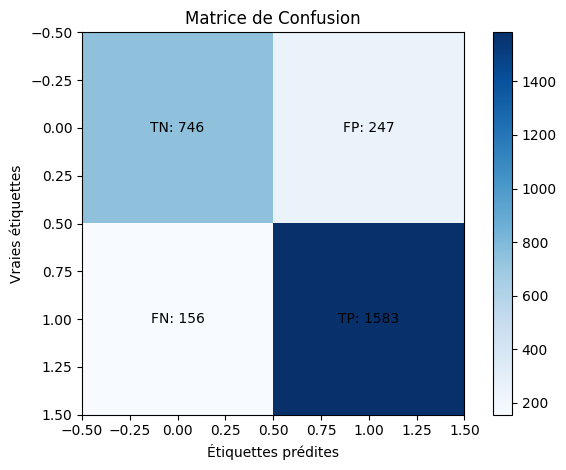
\includegraphics[width=0.8\textwidth]{project_report/figures/RNN_sentiment_matrice.png}
        \caption{\textit{Matrice de confusion du modèle RNN-LSTM}.}
        \label{fig:figureNBVV}
    \end{minipage}
\end{figure} 

Pour Adaboost, les performances sont moyennes par rapport à d’autre modèles, il a démontré une capacité à améliorer progressivement la précision de la classification en agrégeant plusieurs classificateurs faibles, cependant son efficacité peut être limitée dans des cas ou les données sont déséquilibrées où lorsque les caractéristiques discriminantes sont difficiles à extraire ce qui peut entrainer une performance moins satisfonte par rapport à d’autre modèles.\par


Bien que le modèle RNN-LSTM ait produit des résultats solides, il moins performant que des modèles tels que NusSVC et la régression logistique dans ce cas en raison de plusieurs facteurs ; la performance des modèles peut être influencée par la qualité des données d'entraînement, et la répartition déséquilibré des classes qui pose un défi lors de la création de modèle, car les algorithmes ont tendance à favoriser les classes majoritaires et peuvent avoir des performances médiocres pour les classes minoritaires.   




%%%%%%%%%%%%%%%%%%ù ANALYSE DES EMOTIONS %%%%%%%%%%%%

\section{Analyse des émotions}
\subsection{Analyse éxploratoire}

\begin{figure}[h]
    \centering
    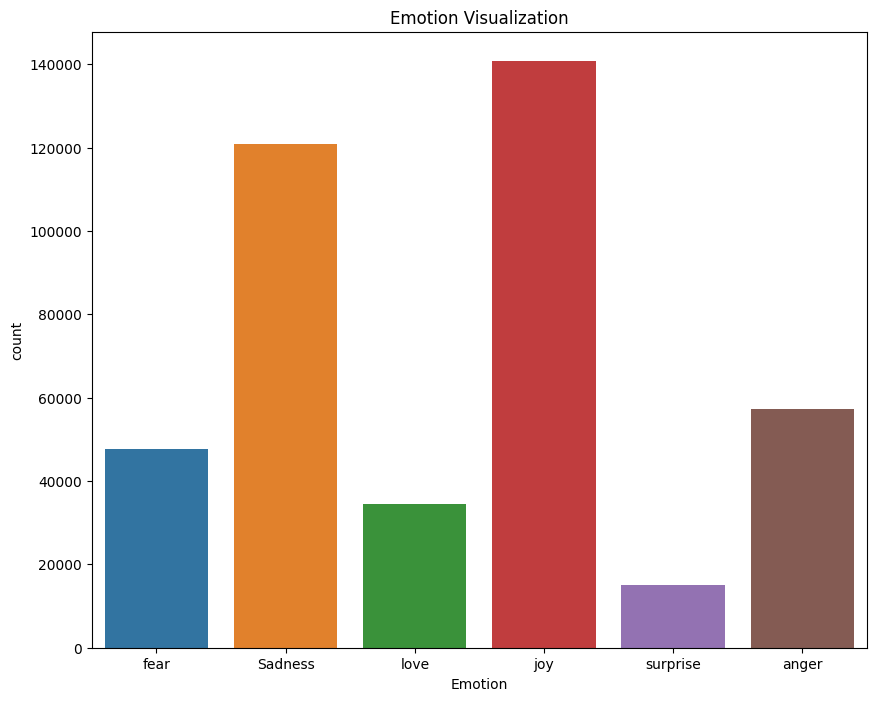
\includegraphics[width=0.7\linewidth]{project_report/figures/repartition-emotion.png}
    \caption{Distribution des classes dans l'ensemble de données Emotions.}
    \label{fig:figDescri}
\end{figure}

%%%%%%%%%%%%%%%%%%%%%%%%%%%%%%%%%%%%%%%%%%%%%%%%%%%%%
Les classes de différentes émotions sont représentées d’une manière inégale, cela signifie plusieurs classes ont beaucoup plus d’exemples que d’autres, créant un déséquilibre significatif. 

\subsection{Nettoyage des données} 
L'étape de nettoyage des données effectuée dans l'analyse des émotions est similaire à celle de l'analyse des sentiments. Dans les deux cas, l'objectif principal est de préparer les données textuelles brutes en éliminant les éléments indésirables et en les rendant prêtes à être analysées par les modèles d'apprentissage automatique ou les techniques d'analyse


\subsection{Préparation des données}
L’application de stemming et lemmatisation sur le dataset des émotions a donné des résultats différents. Lorsque nous avons utilisé la lemmatisation pour le nettoyage des données les performances ont augmenté, tandis que lorsque nous avons appliqué le stemming les performances ont diminué, cela peut s’expliqué par le bon fonctionnement de la lemmatisation qui prend en considération le contexte grammatical et les relations linguistique, par rapport au stemming qu’est moins précis et peut entrainer une perte de sens contextuel et une diminution de performance de modèle utilisé.

\subsection{Représentation textuelle}
Pour le dataset des émotions, l'application des deux techniques de représentation textuelle a donné des résultats différents. L'utilisation de TF-IDF a diminué la performance des modèles par rapport à l'utilisation du vecteur de comptage (CountVectorizer). Cela peut s'expliquer par la nature des émotions, qui sont souvent exprimées par des termes spécifiques. TF-IDF peut diluer l'importance de ces termes en pondérant moins les mots fréquents, ce qui est contre-productif si ces derniers sont précisément ceux qui expriment des émotions importantes. De plus, l'utilisation de bigrammes et de trigrammes a également dégradé la performance des modèles.
%%%%%%%%%%%%%%%%%%%ù TABLE %%%%%%%%%%%%%%%%%%%%%%
\begin{table}[h!]
    \centering
    \caption{Performance des modèles avec CountVectorizer}
    \begin{tabular}{lcccccccc}
        \toprule
        & \multicolumn{4}{c}{CountVectorizer} \\
        \cmidrule(lr){2-5}
        Métriques & Accuracy & Précision & Recall & F1-score \\
        \midrule
        RL & 89\% & 89\% & 89\% & 89\% \\
        CNB & 89\% & 89\% & 89\% & 89\% \\
        MNB & 86\% & 86\% & 86\% & 86\% \\
        \bottomrule
    \end{tabular}
\end{table}

\begin{table}[h!]
    \centering
    \caption{Performance des modèles avec TF-IDF vectorizer}
    \begin{tabular}{lcccccccc}
        \toprule
        & \multicolumn{4}{c}{TF-IDF vectorizer} \\
        \cmidrule(lr){2-5}
        Métriques & Accuracy & Précision & Recall & F1-score \\
        \midrule
        RL & 89\% & 89\% & 89\% & 89\% \\
        CNB & 88\% & 88\% & 88\% & 88\% \\
        MNB & 76\% & 80\% & 73\% & 76\% \\
        \bottomrule
    \end{tabular}
\end{table}
%%%%%%%%%%%%%%%%%%%%%%%%%
\newpage
\subsection{Division des données}
Les résultats obtenus mettent en évidence la stabilité des performances des modèles de régression logistique et de complément naïf bayésien lorsqu'ils sont soumis à des variations de la taille de l'ensemble de test pour le jeu de données sur les émotions. Ces observations indiquent que les modèles conservent une cohérence dans leurs capacités prédictives, peu importe la taille des données de test. Malgré de légères fluctuations dans les métriques d'évaluation telles que l'accuracy, le recall, la précision et le F1-score, les performances globales des deux modèles restent relativement constantes sur différentes tailles d'ensemble de test. Cette constance suggère une certaine robustesse des modèles face aux changements de taille des données de test, ce qui renforce leur capacité à généraliser efficacement sur de nouveaux ensembles de données. En somme, ces résultats démontrent la fiabilité des modèles de régression logistique et de complément naïf bayésien dans leur capacité à maintenir des performances stables et cohérentes, ce qui les rend pertinents pour une utilisation dans divers contextes d'analyse des émotions. 
%%%%%%%%%%%%%%%%%%%ù TABLE %%%%%%%%%%%%%%%%%%%%%%
\begin{table}[h!]
    \centering
    \caption{Modèle de régression logistique}
    \begin{tabular}{lcccc}
        \toprule
        Test\_size & Accuracy & Recall & Précision & F1\_score \\
        \midrule
        0.1 & 0.88 & 0.88 & 0.88 & 0.88 \\
        0.2 & 0.89 & 0.89 & 0.89 & 0.89 \\
        0.3 & 0.89 & 0.89 & 0.89 & 0.89 \\
        0.4 & 0.89 & 0.89 & 0.89 & 0.89 \\
        \bottomrule
    \end{tabular}
\end{table}

\begin{table}[h!]
    \centering
    \caption{Modèle de complément NB }
    \begin{tabular}{lcccc}
        \toprule
        Test\_size & Accuracy & Recall & Précision & F1\_score \\
        \midrule
        0.1 & 0.85 & 0.86 & 0.90 & 0.88 \\
        0.2 & 0.88 & 0.88 & 0.88 & 0.88 \\
        0.3 & 0.85 & 0.86 & 0.90 & 0.88 \\
        0.4 & 0.88 & 0.88 & 0.88 & 0.88 \\
        \bottomrule
    \end{tabular}
\end{table}

\subsection{La classification}
Pour la classification des émotions en plusieurs catégories (joie, amour, colère, surprise, tristesse et peur), nous utilisons des algorithmes d'apprentissage supervisé ainsi que des algorithmes de réseaux de neurones tels que :
\begin{itemize}
    \item Régression logistique;
    \item Naïve Bayes multinomial;
    \item Naïve Bayes complément;
    \item Adaboost;
    \item RNN-LSTM;
    \item CNN.
\end{itemize}
En suivant la même méthodologie d’analyse des sentiments précédente, nous évaluons les classificateurs des émotions en calculant les métriques de performance et en visualisant la matrice de confusion et le graphique des performances pour les réseaux de neurones. \\
Les résultats obtenus à partir des modèles mentionnés seront détaillés dans les sections suivantes, où nous examinerons en profondeur les performances de chaque approche. Chaque modèle sera évalué en fonction de critères tels que la précision, le rappel, la F-mesure et d'autres métriques pertinentes. En outre, nous analyserons les forces et les faiblesses de chaque méthode, en mettant en lumière les aspects clés de leur mise en œuvre et de leur interprétation. Ce niveau de détail permettra une compréhension approfondie des performances de chaque modèle, ainsi que des recommandations pour leur utilisation future dans des scénarios similaires.


\subsection{Résultats et discussion}

%%%%%%%%%%%%%%%%ù TABLE OF RESULTS %%%%%%%%%%%%%%%
\begin{table}[h!]
    \centering
    \caption{Performance des modèles pour le dataset des émotions}
    \label{tab:Em}
    \begin{tabular}{lcccc}
        \toprule
        Dataset des émotions & Accuracy & Precision & Recall & F1-score \\
        \midrule
        Model 1 : RNN\_LSTM & 93\% & 93\% & 93\% & 93\% \\
        Modèle 2 : MNB & 76\% & 80\% & 76\% & 76\% \\
        Modèle 3 : RL & 89\% & 89\% & 89\% & 89\% \\
        Modèle 4 : CNB & 88\% & 88\% & 88\% & 88\% \\
        Modèle 5 : CNN & 93\% & 93\% & 93\% & 93\% \\
        Modèle 6 : AdaBoost & 0.36\% & 24\% & 24\% & 21\% \\
        \bottomrule
    \end{tabular}
\end{table}
%%%%%%%%%%%%%%%%%%%%%%% END OF TABLE %%%%%%%%%%
En se basant sur les résultats obtenus dans les trois modèles (Voir le tableau [\ref{tab:Em}] (Naïve Bayes complément, Naïve Bayes multinomial et la régression logistique), on peut donner les mêmes interprétations obtenues déjà dans le dataset précédent. Cependant, on peut ajouter que le Naïve Bayes complément (CNB) et la régression logistique sont capables de s'adapter à des datasets complexes et volumineux, tout en générant rapidement des résultats en comparaison avec des algorithmes plus lents mais performants.\par
\begin{figure}[h]
    \centering
    \begin{minipage}{0.45\textwidth}
        \centering
        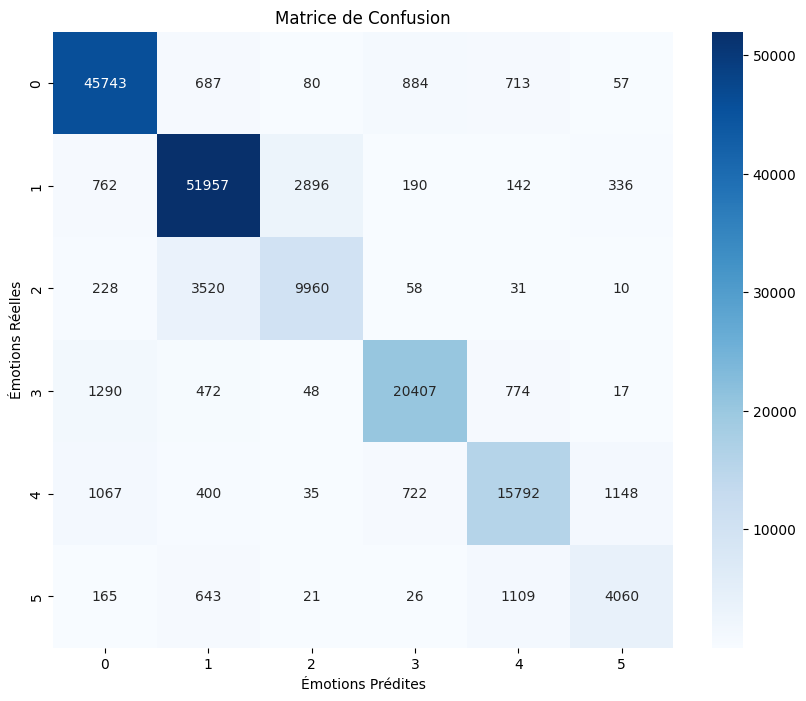
\includegraphics[width=\textwidth]{project_report/figures/matrice-complement NB-emotion.png}
        \caption{\textit{Matrice de confusion du modèle CNB}.}
        \label{fig:figureSHJJJR}
    \end{minipage}\hfill
    \begin{minipage}{0.45\textwidth}
        \centering
        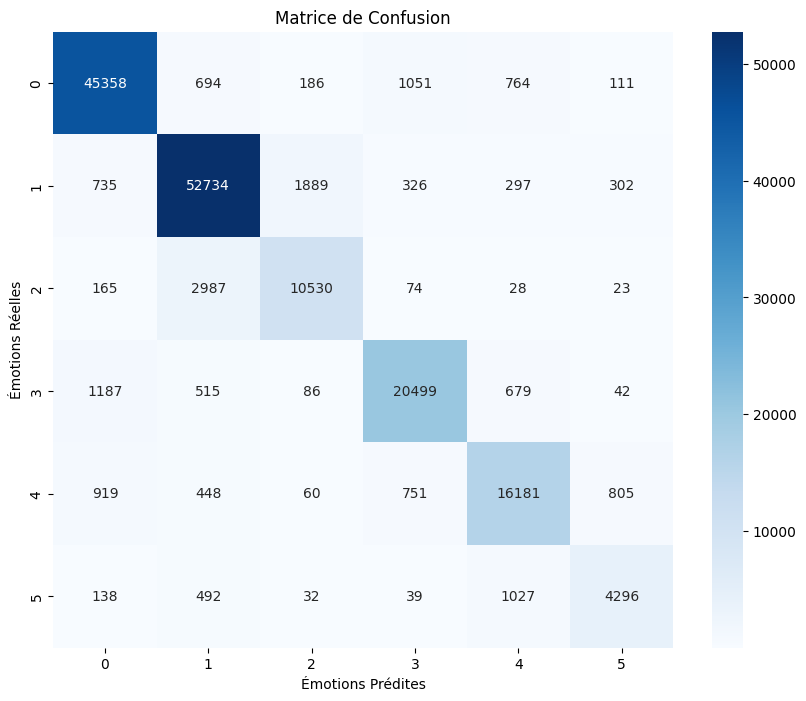
\includegraphics[width=\textwidth]{project_report/figures/RL-matrice-emotion.png}
        \caption{\textit{Matrice de confusion du modèle RL}.}
        \label{fig:figureNBVV}
    \end{minipage}
\end{figure} 


Les performances comparables du CNN et du RNN-LSTM sur le dataset des émotions suggèrent que ces deux architectures sont également efficaces pour traiter ce type de données. Bien que le CNN soit généralement considéré comme plus adapté pour l'extraction de caractéristiques locales à partir de données structurées, et que le RNN-LSTM soit privilégié pour modéliser les dépendances séquentielles à long terme, les résultats montrent que les deux approches sont capables de capturer efficacement les informations pertinentes pour la classification des émotions. Cette observation met en lumière la flexibilité et la robustesse des réseaux de neurones profonds, qui peuvent s'adapter à différents types de données et produire des performances comparables dans des contextes variés.\par
%%%%%%%%%%%%%%ùùùFIG 
\begin{figure}[h]
    \centering
    \begin{minipage}{0.45\textwidth}
        \centering
        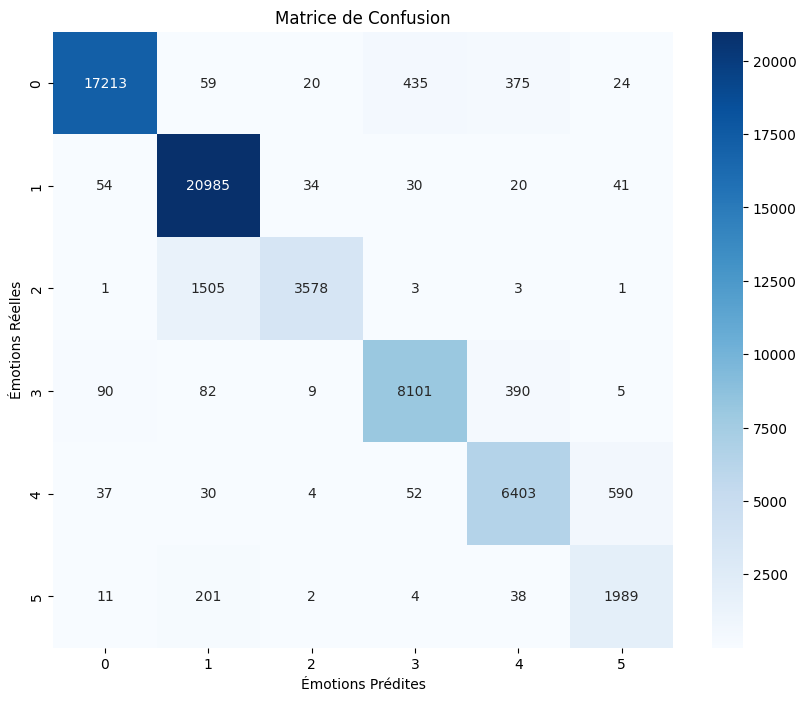
\includegraphics[width=\textwidth]{project_report/figures/CNN_matrice_emotion.png}
        \caption{\textit{Matrice de confusion du modèle CNN}.}
        \label{fig:figureCNN}
    \end{minipage}\hfill
    \begin{minipage}{0.45\textwidth}
        \centering
        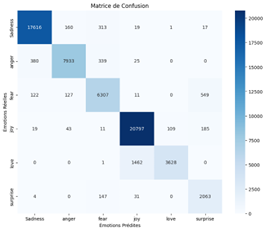
\includegraphics[width=\textwidth]{project_report/figures/emotion_rnn.png}
        \caption{\textit{Matrice de confusion du modèle RNN-LSTM}.}
        \label{fig:figureLSTM}
    \end{minipage}
\end{figure} 



%%%%%%%%%%%%%%%%%FIG 
Malgré l'augmentation du nombre d'estimateurs pour le modèle créé en utilisant le classificateur AdaBoost et l'utilisation de la validation croisée, les performances restent en deçà des attentes.
Cette situation peut être attribuée à plusieurs facteurs, tels que la complexité inhérente des données qui peut rendre l'application de modèles tels qu'AdaBoost mal adaptée, ainsi que le déséquilibre entre les classes.

\begin{figure}[h]
    \centering
    \begin{minipage}{0.45\textwidth}
        \centering
        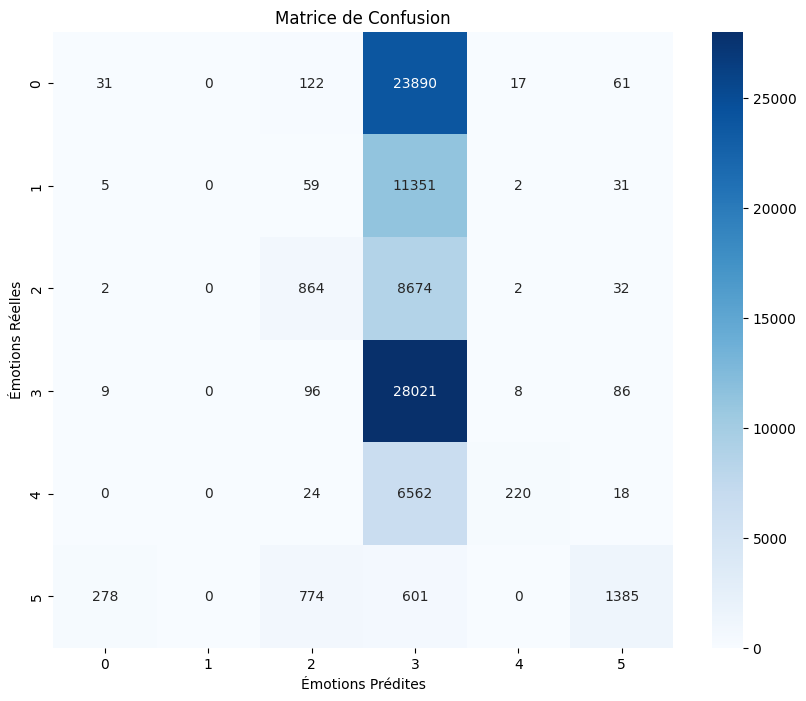
\includegraphics[width=\textwidth]{project_report/figures/adaboost_matrice_emotion.png}
        \caption{\textit{Matrice de confusion du modèle AdaBoost}.}
        \label{fig:figureSHJJJR}
    \end{minipage}\hfill
    \begin{minipage}{0.45\textwidth}
        \centering
        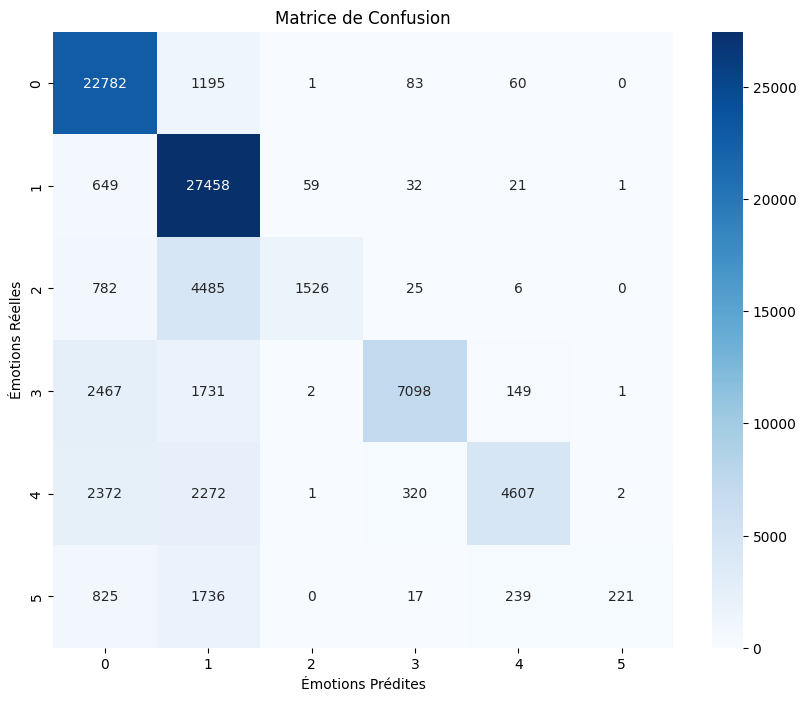
\includegraphics[width=\textwidth]{project_report/figures/multinomial NB-emotion_matrice.png}
        \caption{\textit{Matrice de confusion du modèle MNB}.}
        \label{fig:figureNBVV}
    \end{minipage}
\end{figure} 


\section{Déploiement de l'application}
\subsection{Modélisation}
\textbf{Le langage de Modélisation Unifié UML}
, communément appelé UML, constitue l'un des langages les plus essentiels lorsqu'il s'agit d'initier un projet. Il se révèle être un langage graphique de modélisation fondé sur des symboles graphiques soigneusement élaborés pour offrir une méthode standardisée permettant de visualiser la conception d'un système.
L'UML est employé pour ajuster, représenter, définir et élaborer les documents indispensables à la réalisation réussie d'un projet. Il instaure une norme de modélisation, offrant une représentation architecturale du logiciel. Parmi les divers éléments pouvant être représentés, on compte :
\begin{itemize}
    \item Les activités d'un objet ou d'un logiciel.
    \item Les intervenants (acteurs) du système.
    \item Les processus en cours.
    \item Les schémas de bases de données.
    \item Les éléments constitutifs du logiciel.
    \item La réutilisation de composants existants.
\end{itemize}
Les outils de modélisation UML autorisent même la génération automatique de tout ou partie du code d'une application logicielle, tel que le langage Java, en se basant sur les différents documents conçus.
Pour comprendre l'architecture de notre projet, nous nous sommes servis de deux types de diagramme. La suite explique ceci en détail. \par
\textbf{Diagramme de cas d'utilisation}
\begin{figure}[h]
    \centering
    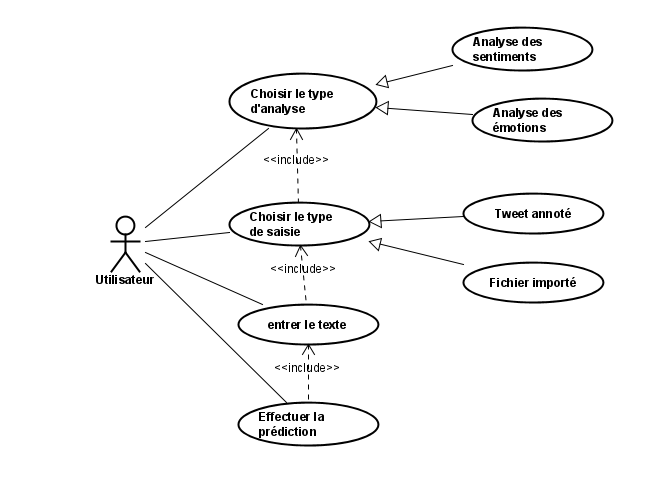
\includegraphics[width=0.7\linewidth]{project_report/figures/Capture d’écran (1208).png}
    \caption{\textit{Diagramme de cas d'utilisation}}
    \label{fig:figUsecase}
\end{figure}
\\Dans un langage UML, les diagrammes de cas d'utilisation modélisent le comportement d'un système et saisissent les exigences de celui-ci. Ils sont utilisés pour décrire le fonctionnement du système et son utilisation par les acteurs, mais sans démontrer comment le système fonctionne à l'interne.
Afin de décrire l'ensemble des fonctions générales et de l'étendue de notre système, nous nous sommes servis du diagramme de cas d'utilisation ci-dessous, qui identifie également les interactions entre le système et ses acteurs.
La Figure [\ref{fig:figUsecase}] présente le schéma global du diagramme de cas d'utilisation de notre système. 


\textbf{Diagramme de séquence}
Les diagrammes de séquence UML sont des outils graphiques d'interaction qui fournissent une vue approfondie sur la manière dont les actions sont exécutées. Ils saisissent l'interrelation entre les objets au sein d'une collaboration donnée. Ces diagrammes ont également une dimension temporelle, mettant en évidence la séquence des interactions par le biais de l'axe vertical du schéma pour représenter le passage du temps, les messages échangés et leur timing respectif. 
La figure [\ref{fig:figsequence}] présente le diagramme de séquence de notre interface :

\begin{figure}[h]
    \centering
    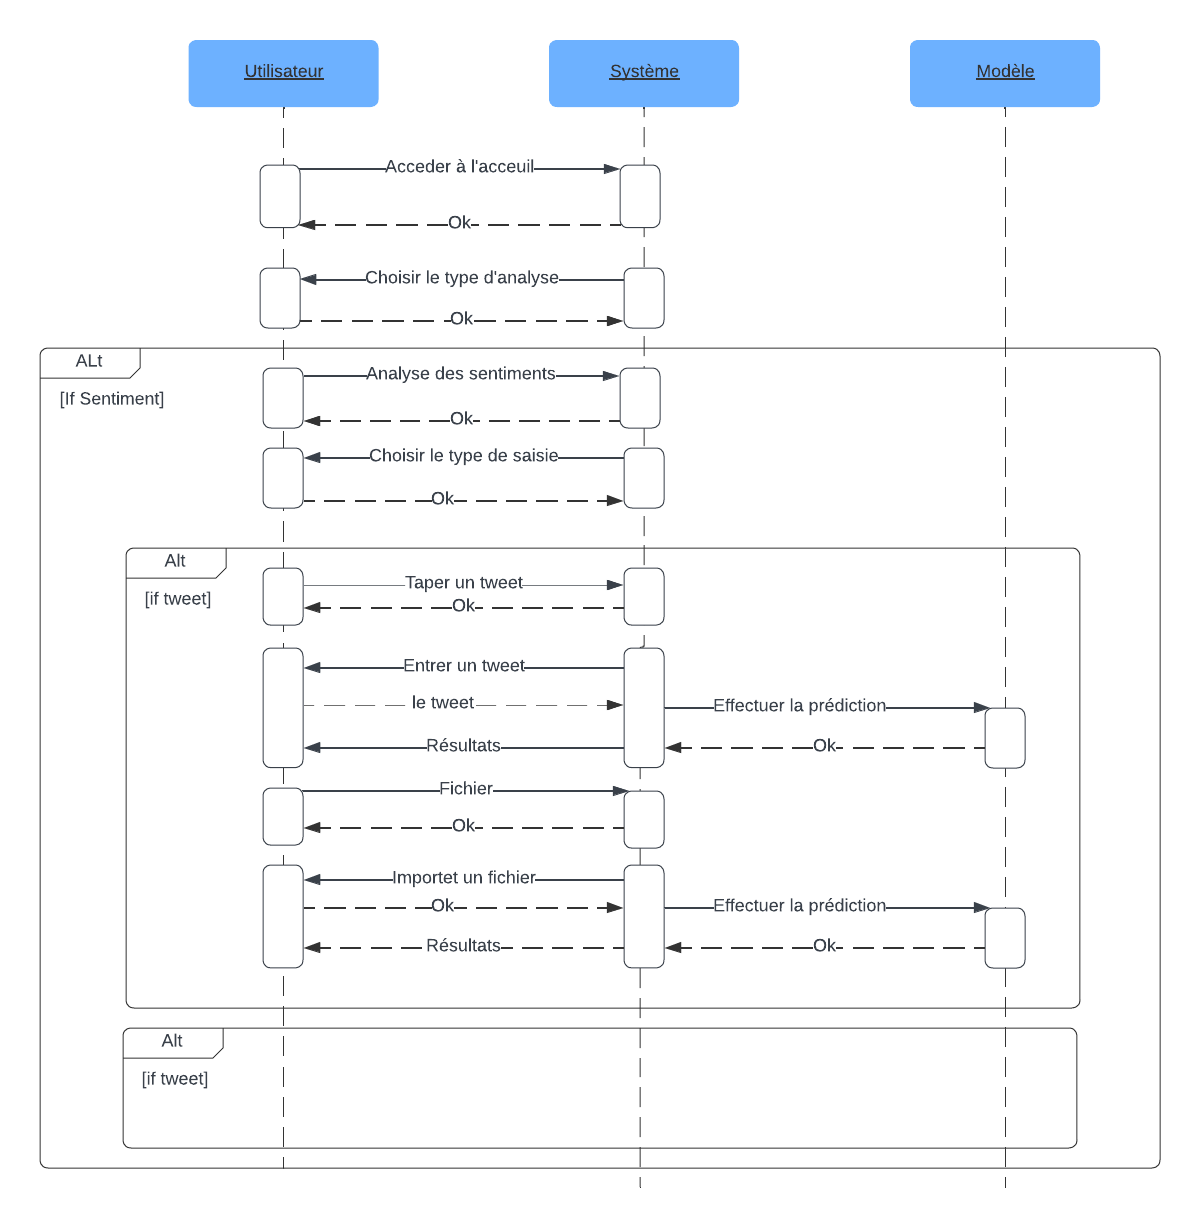
\includegraphics[width=1\linewidth]{project_report/figures/Sequence diagram (3).png}
    \caption{\textit{Diagramme de séquence}}
    \label{fig:figsequence}
\end{figure}


Dans la deuxième partie de l'instruction conditionnelle (else), le processus est similaire à celui précédemment décrit, mais cette fois-ci appliqué à l'identification et au traitement des émotions. Les données sont analysées et catégorisées en fonction des différentes émotions exprimées, suivant une approche semblable à celle utilisée pour les sentiments.
\subsection{Archeticture globale de l'application}
La structure ou l’architecture d'une application définit les schémas et les méthodes employés pour concevoir et élaborer une application. Cette structure fournit un guide ainsi que les procédés recommandés à suivre pour créer une application bien organisée.
Le fonctionnement de notre système global peut être résumé selon les étapes illustrées dans la figure ci-dessous. 
\begin{figure}[h]
    \centering
    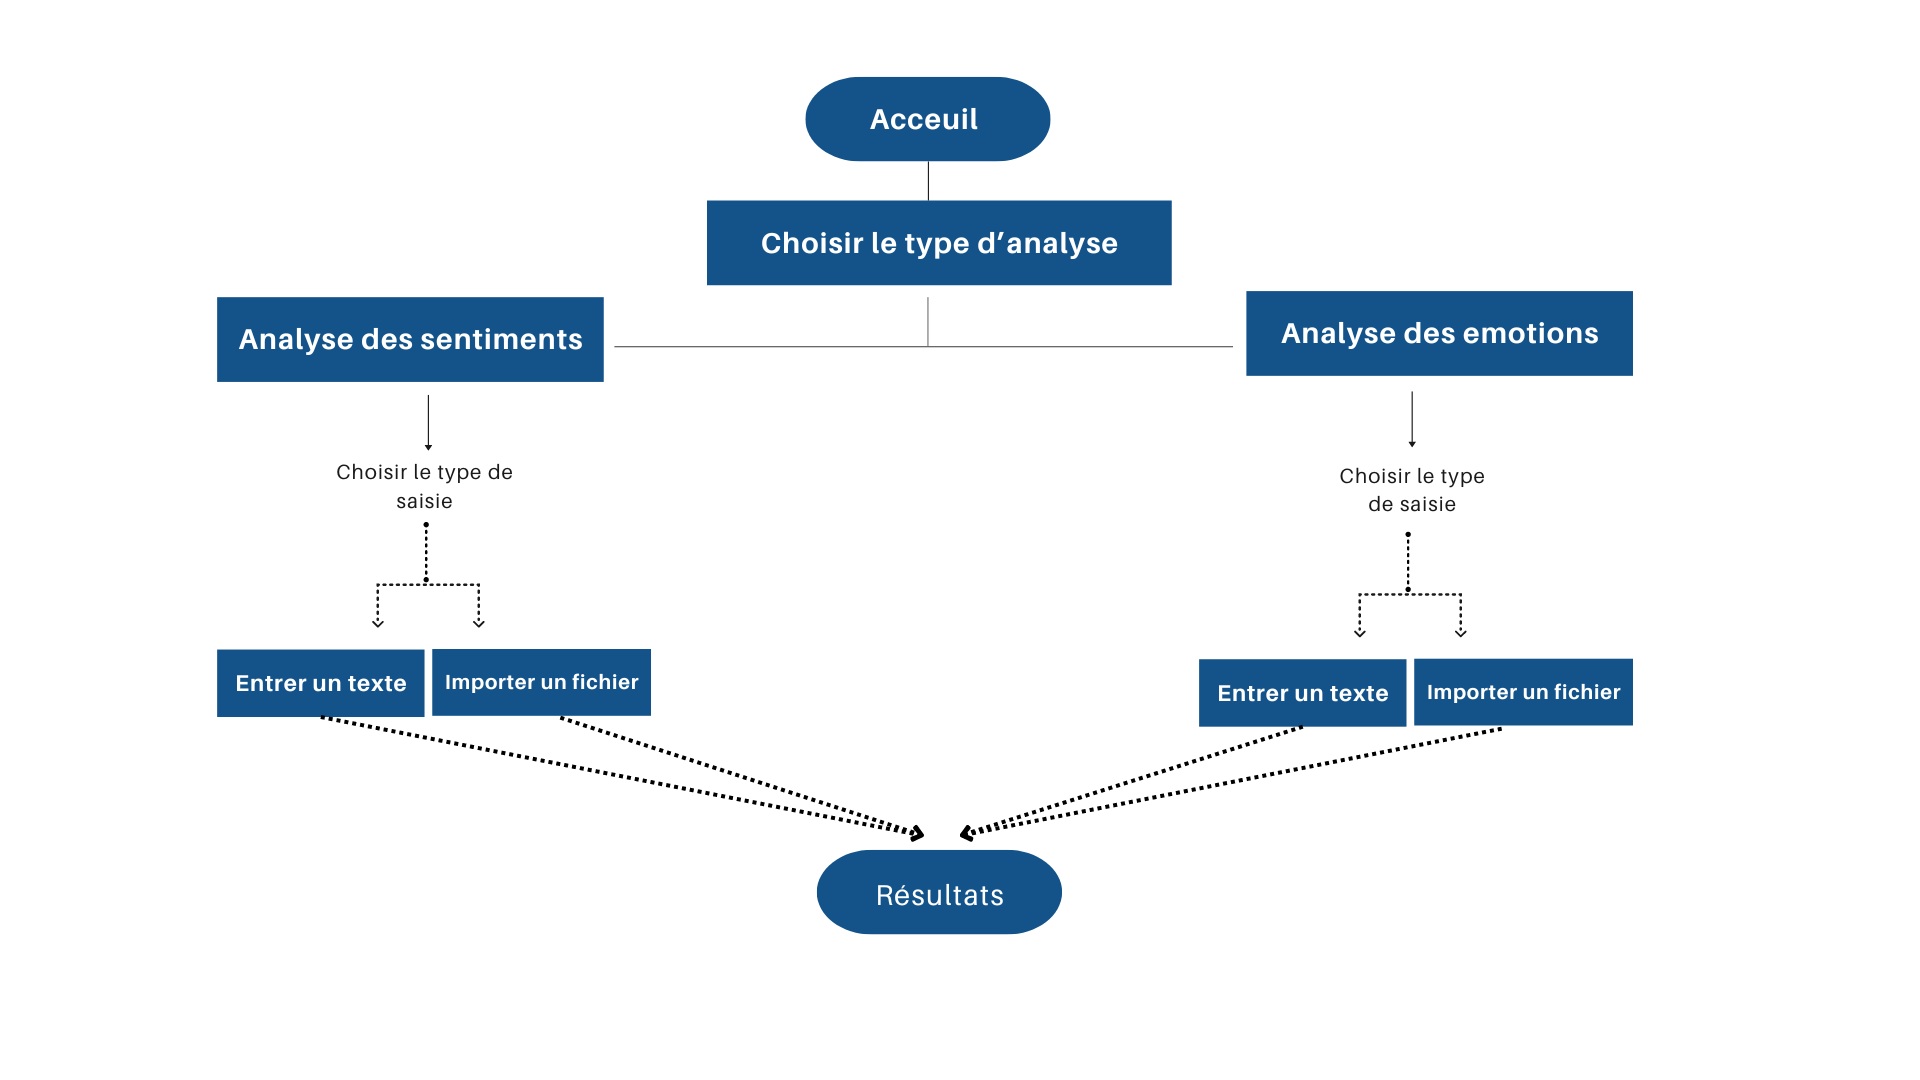
\includegraphics[width=1\linewidth]{project_report/figures/Oui.png}
    \caption{\textit{Archeticture globale de l'application}}
    \label{fig:arch}
\end{figure}
\subsection{Démonstration des interfaces}
\subsubsection{Interface principales}
La première version de cette application permet les fonctionnalités suivantes :
\begin{itemize}
    \item \textbf{Analyse des sentiments et des émotions annotés :} l’application permet aux utilisateurs de taper leurs textes. Une fois le texte est soumis l’application affiche le sentiment ou l’émotion correspondant selon le choix préalable d’utilisateur.
    \item \textbf{Analyse des sentiments et des émotions à partir des fichiers Excel ou csv :} l’application permet aux utilisateurs d’importer des fichiers contenants des tweets, le système analyse ces données et affiche les résultats avec des statistiques.
\end{itemize}
Cette interface [\ref{fig:acc}] ouffre a l'utilisateur la possibilité de choisir le type de saisie. L'utilisateur peut choisir entre deux options de saisie : saisie manuelle ou importation de fichier. Cette zone permet à l'utilisateur de sélectionner le mode de saisie qui lui convient le mieux.

\begin{figure}[h]
    \centering
    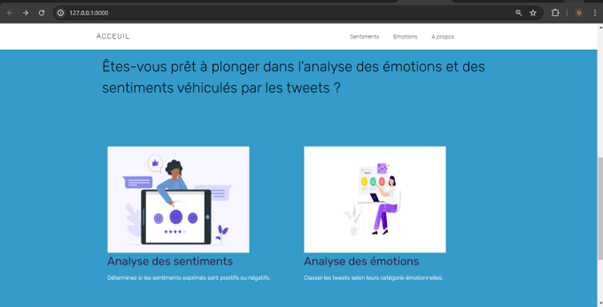
\includegraphics[width=0.9\linewidth]{project_report/figures/Acc2.png}
    \caption{\textit{Interface 1: Choix de type de saisie}}
    \label{fig:acc}
\end{figure}



\subsubsection{Interfaces d'importation des données}
\begin{figure}[h]
    \centering
    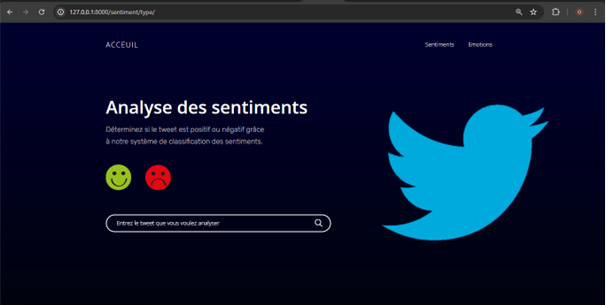
\includegraphics[width=0.9\linewidth]{project_report/figures/entrer un text.png}
    \caption{\textit{Interface 2: saisir un texte.}}
    \label{fig:text}
\end{figure}
Cette interface [\ref{fig:text}] offre à l'utilisateur la possibilité d'analyser les sentiments d'un texte. Voici les fonctionnalités qu'elle offre :
\begin{enumerate}
    \item \textbf{Zone de saisie de texte : }Si l'utilisateur choisit la saisie manuelle, il peut saisir un tweet ou tout autre texte dans cette zone dédiée. Cette fonctionnalité permet une analyse en temps réel des sentiments du texte saisi.
    \item \textbf{Bouton d'analyse :} Une fois que l'utilisateur a entré le texte, il peut cliquer sur ce bouton entrer pour lancer le processus d'analyse des sentiments. Après l'analyse, les résultats sont affichés à l'utilisateur.
    \item \textbf{Option d'importation de fichier :} Si l'utilisateur choisit d'importer un fichier, il peut cliquer sur cette option pour sélectionner un fichier texte contenant plusieurs tweets à analyser en une seule fois. Cela offre une flexibilité supplémentaire pour l'analyse de gros volumes de données.
\end{enumerate}
Pour le choix le l'analyse des émotions l'utilisateur peut aussi choisir le type de saisie (Voir la figure [\ref{fig:tem}]): 
\begin{figure}[h]
    \centering
    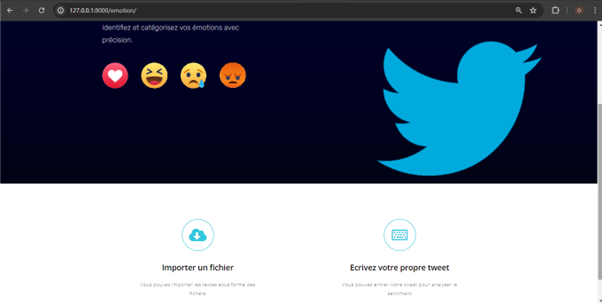
\includegraphics[width=0.9\linewidth]{project_report/figures/choix emotion.png}
    \caption{\textit{Interface 3: Choix de type de saisie.}}
    \label{fig:tem}
\end{figure}\\
Après que l'utilisateur a fait son choix concernant le type de saisie, les fonctionnalités de cette interface sont les mêmes que celles de l'analyse des sentiments. L'utilisateur peut soit entrer un texte manuellement dans la zone de saisie dédiée, soit importer un fichier (Voir la figure [\ref{fig:fechtt}]) contenant plusieurs textes à analyser. Dans les deux cas, l'utilisateur peut lancer l'analyse en cliquant sur le bouton entrer. Une fois l'analyse terminée, les résultats sont affichés de manière claire et concise, avec des visualisations graphiques et des statistiques détaillant les pourcentages de sentiments positifs et négatifs.
\begin{figure}[h]
    \centering
    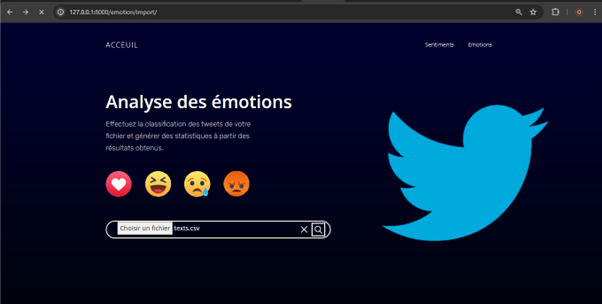
\includegraphics[width=0.9\linewidth]{project_report/figures/file.png}
    \caption{\textit{Interface 4: importer un fichier .}}
    \label{fig:fechtt}
\end{figure}
\subsection{Interface des resultats}
\begin{figure}[h]
    \centering
    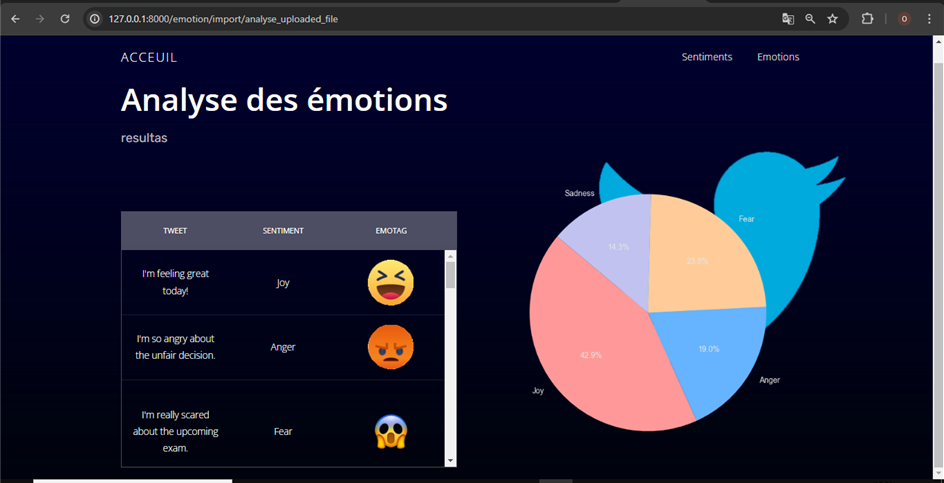
\includegraphics[width=0.9\linewidth]{project_report/figures/resultatsem.png}
    \caption{\textit{Interface 6: Résultat d'un fichier importé.}}
    \label{fig:emmmm}
\end{figure}
Pour les textes saisis, l'interface des résultats montre si le texte est positif ou négatif (Voir la figure [\ref{fig:sennnn}]), accompagné d'un emoji descriptif. Cela permet à l'utilisateur de comprendre rapidement l'émotion générale exprimée dans le texte de manière visuelle et intuitive.
\begin{figure}[h]
    \centering
    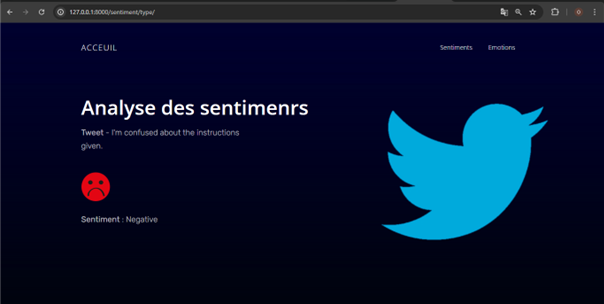
\includegraphics[width=0.9\linewidth]{project_report/figures/resultatssenn.png}
    \caption{\textit{Interface 5: Résultat d'un texte saisie.}}
    \label{fig:sennnn}
\end{figure}

Pour les fichiers importés, l'interface des résultats affiche un tableau détaillant les différentes sentiments et émotions prédites. En complément, un diagramme circulaire (pie chart) est présenté pour illustrer les statistiques des différentes émotions détectées dans l'ensemble du fichier (Voir la figure [\ref{fig:emmmm}]). Cette présentation visuelle offre une vue d'ensemble claire et facile à interpréter des émotions dominantes, facilitant l'analyse des données en masse.






\newpage


\textbf{Conclusion}\par
En conclusion, ce chapitre a présenté les résultats de notre projet, en mettant en évidence les performances des modèles et en comparant les résultats obtenus. Ces résultats fournissent des informations précieuses sur l'efficacité de nos approches et nous permettent de mieux comprendre les défis et les opportunités dans le domaine de l'analyse des sentiments et des émotions. Alors que nous continuons à développer notre projet et à explorer de nouvelles avenues de recherche, les résultats présentés dans ce chapitre serviront de base solide pour guider nos futurs efforts et initiatives dans ce domaine en constante évolution.





\clearpage
\phantomsection
\addcontentsline{toc}{chapter}{CONCLUSION ET PERSPECTIVES}
\chapter*{CONCLUSION ET PERSPECTIVES}
\lettrine[lines=1,lraise=0.1,findent=0.6em]{D}{ans} ce rapport, nous avons présenté notre projet d'analyse des sentiments et des émotions exprimés dans les tweets. Nos résultats ont montré que cette approche permet de mieux comprendre les réactions du public sur différents sujets. Cependant, des améliorations sont encore nécessaires, notamment dans la gestion de la négation, afin d'affiner davantage la compréhension des sentiments.

Une perspective intéressante serait de permettre à l'utilisateur de choisir le modèle d'analyse à appliquer depuis notre application, offrant ainsi une plus grande flexibilité. De plus, l'extension de notre analyse à d'autres sources de données, comme les commentaires de réseaux sociaux ou les avis en ligne, pourrait apporter une vision plus globale des tendances émotionnelles. Enfin, l'intégration de techniques d'apprentissage machine plus avancées pourrait contribuer à une classification encore plus précise des sentiments exprimés.

En outre, une idée prometteuse consisterait à entraîner le modèle en anglais, puis lorsque l'utilisateur entre un texte en français, une traduction serait effectuée avant de procéder à l'analyse des sentiments. Cette approche bilingue pourrait étendre considérablement la portée de notre application et en améliorer l'utilité pour les utilisateurs francophones.


\input{sec/references}

\newpage
\appendix
\addtocounter{chapter}{1}

%%%%%%%%%%%%%%%%%%%% BIBLIO 
\newpage
\phantomsection
\addcontentsline{toc}{chapter}{REFERENCES}


\nocite{* BIBIOGRAPHY}
\renewcommand{\bibname}{REFERENCES}
\bibliographystyle{IEEEtran}
\bibliography{biblio}
\printbibligraphy
\end{document}
